\documentclass[12pt]{book}
\usepackage[utf8]{inputenc}
\usepackage[T1]{fontenc}
\usepackage{lmodern}        % Fuentes vectoriales Type 1 (igual que Cap 3)
\usepackage{microtype}      % Mejora la legibilidad
\usepackage[spanish]{babel}
\usepackage[margin=2.5cm]{geometry}
\usepackage{amsmath}
\usepackage{amssymb}
\usepackage{graphicx}
\usepackage{booktabs}
\usepackage{tabularx}
\usepackage{sidecap}
\usepackage{threeparttable}
\usepackage{enumitem}
\usepackage{mathptmx}

\graphicspath{{imagenes/}}

\AtBeginDocument{\shorthandoff{"}}

\begin{document}

\setcounter{chapter}{1}

% --- INICIO DEL CAPÍTULO 2 ---
\chapter{Estática del Cuerpo}

\begin{flushleft}
    \textit{La estática del cuerpo se investiga revisando primero las fuerzas, los torques y el equilibrio, y luego aplicando estas condiciones a la estática en un plano y a la palanca. Se analizan ejemplos específicos de estática en el cuerpo, incluyendo los del antebrazo, las caderas, el hombro, la rodilla, el tobillo, las mandíbulas y la parte baja de la espalda. Algunos de estos están relacionados con lesiones en el cuerpo, como las de las caderas y la parte baja de la espalda. Varias de las discusiones en este capítulo forman la base para analizar el movimiento en el siguiente capítulo.}
\end{flushleft}

\hrule
\vspace{1em}

El estudio del balance de fuerzas de un objeto en reposo se llama «estática». Además, el estudio del movimiento muy lento normalmente puede tratarse como una serie de condiciones estáticas ---como si no hubiera movimiento---; esto se llama «cuasiestática». Después de revisar las condiciones para el equilibrio estático en tres dimensiones, examinaremos la simplificación útil a dos dimensiones, cuyos ejemplos a menudo se pueden caracterizar como uno de los tres tipos de palancas. Luego aplicaremos estas condiciones de equilibrio al antebrazo, la cadera y la columna vertebral (parte baja de la espalda). La estática es un área importante de la biomecánica \cite{15, 24, 28, 38}.

\section{Revisión de fuerzas, torques y equilibrio}

Cada fuerza $\vec{\mathbf{F}}$ se puede resolver en componentes en las direcciones $x$, $y$ y $z$ ($F_x$, $F_y$, $F_z$). En una condición estática, la suma de las fuerzas $\vec{\mathbf{F}}$ en cada una de las direcciones $x$, $y$ y $z$ es cero:
\begin{align}
\sum F_x &= 0, \nonumber \\
\sum F_y &= 0, \nonumber \\
\sum F_z &= 0.
\label{eq:2.1}
\end{align}
La velocidad del centro de masa del objeto en cada dirección es entonces constante, y aquí normalmente se asumirá que es cero. Estas fuerzas pueden estar en equilibrio ya sea para todo el cuerpo o para cualquier parte del mismo.

De manera similar, cada torque $\vec{\boldsymbol{\tau}}$ se puede resolver en componentes en las direcciones $x$, $y$ y $z$ ($\tau_x$, $\tau_y$, $\tau_z$). En una condición estática, los torques $\vec{\boldsymbol{\tau}}$ alrededor de los ejes $x$, $y$ y $z$ también suman cero para todo el cuerpo y para cualquier parte del cuerpo:
\begin{align}
\sum \tau_x &= 0, \nonumber \\
\sum \tau_y &= 0, \nonumber \\
\sum \tau_z &= 0.
\label{eq:2.2}
\end{align}
La velocidad de rotación angular del objeto alrededor de cada eje es entonces constante, y aquí normalmente se asumirá que es cero.

¿Qué es en realidad un torque? Las fuerzas describen cambios en el movimiento lineal ---lo que significa cambios en las velocidades---, mientras que los torques describen cómo estas mismas fuerzas pueden cambiar el movimiento angular ---lo que significa cambios en las velocidades angulares---. El diagrama en la Fig. 2.1b muestra que una fuerza $\vec{\mathbf{F}}$ aplicada en la dirección $y$ positiva (con componente $F$) a una distancia $+r$ del eje $z$, lleva a un torque alrededor del eje $z$, $\tau_z$, de magnitud $r F$. Esto conduce a un movimiento en sentido antihorario, causado por una aceleración angular que aumenta el ángulo $\theta$. Esto se define como un torque positivo alrededor de este eje. Ocurriría un torque negativo, por ejemplo, si la fuerza se aplicara en la dirección $y$ negativa. Esto conduciría a un movimiento en sentido horario, causado por una aceleración angular que disminuye el ángulo $\theta$ (con signo).

En general, el torque (vector $\vec{\boldsymbol{\tau}}$) alrededor de cualquier eje se define como el producto cruz vectorial entre el vector de distancia desde ese eje hasta el punto donde se aplica la fuerza, $\vec{\mathbf{r}}$, y el vector de fuerza $\vec{\mathbf{F}}$ (Fig. 2.1e):
\begin{equation}
\vec{\boldsymbol{\tau}} = \vec{\mathbf{r}} \times \vec{\mathbf{F}}.
\label{eq:2.3}
\end{equation}
(No es necesario que entienda o utilice este producto cruz vectorial, solo los resultados que se presentan a continuación).

\begin{SCfigure}[0.5][htbp]

  \centering
  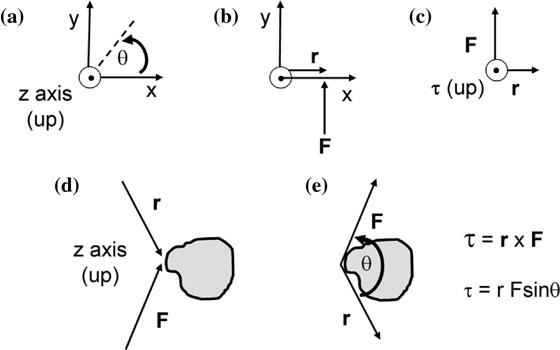
\includegraphics[width=0.55\textwidth]{21.png}
  \caption{Torques y ejes relevantes.}
  \label{fig:21}
\end{SCfigure}



Debido a que los vectores se pueden trasladar a cualquier lugar, las cosas pueden quedar más claras si trasladamos tanto $\vec{\mathbf{r}}$ como $\vec{\mathbf{F}}$, como en la Fig. 2.1b, d, de modo que se originen desde donde se aplica la fuerza, como en la Fig. 2.1c, e, respectivamente. Llamaremos $\theta$ al ángulo desde el vector $\vec{\mathbf{r}}$ al vector $\vec{\mathbf{F}}$. El torque $\tau_z$ sobre el eje ascendente es
\begin{equation}
\tau_z = r F \sin \theta,
\label{eq:2.4}
\end{equation}
donde $r$ es la magnitud del vector $\vec{\mathbf{r}}$ (la distancia desde el eje hasta el punto donde se aplica la fuerza) y $F$ es la magnitud del vector $\vec{\mathbf{F}}$. Para $0^\circ < \theta < 180^\circ$ (o $0 < \theta < \pi$ en radianes), $\sin \theta$ es positivo y el torque es positivo (Fig. 2.2a), mientras que para $180^\circ < \theta < 360^\circ$ ($\pi < \theta < 2\pi$), $\sin \theta$ es negativo y el torque es negativo (Fig. 2.2b). Cuando $\theta = 90^\circ$ ($= \pi/2$), $\sin \theta = 1$ y el torque es $r F$, como se indicó anteriormente. Cuando $\vec{\mathbf{r}}$ y $\vec{\mathbf{F}}$ son paralelos ($\theta = 0^\circ$ ($= 0$)) o antiparalelos ($\theta = 180^\circ$ ($= \pi$)), el torque es cero.

Claramente, solo la componente de $\vec{\mathbf{r}}$ normal a $\vec{\mathbf{F}}$, a la que llamaremos $r'$, contribuye a la acción del torque. De hecho, como lo demuestra la Fig. 2.3, $\tau_z = r' F$. Equivalentemente, solo la componente de $\vec{\mathbf{F}}$ normal a $\vec{\mathbf{r}}$, es decir, $F'$, contribuye a la acción del torque, y $\tau_z = r F'$. Como veremos, a veces se proporciona información donde se dan estas componentes normales de desplazamiento o fuerza, y los torques se pueden calcular sin determinar explícitamente el ángulo entre los vectores de desplazamiento y de fuerza. Por consiguiente,
\begin{equation}
\tau_z = r F \sin \theta = r' F = r F'.
\label{eq:2.5}
\end{equation}
Esto es cierto para cualquier eje. El eje se puede elegir de manera inteligente para un problema particular con el fin de simplificar el análisis.

\begin{figure}[htbp]

  \centering
  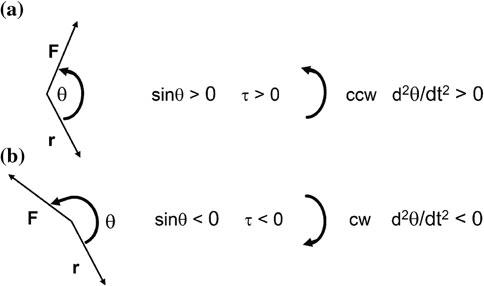
\includegraphics[width=0.75\textwidth]{22.png}
  \caption{Dirección de los torques, mostrando \textbf{a} torques positivos y \textbf{b} torques negativos.}
  \label{fig:22}
\end{figure}

\begin{figure}[htbp]

  \centering
  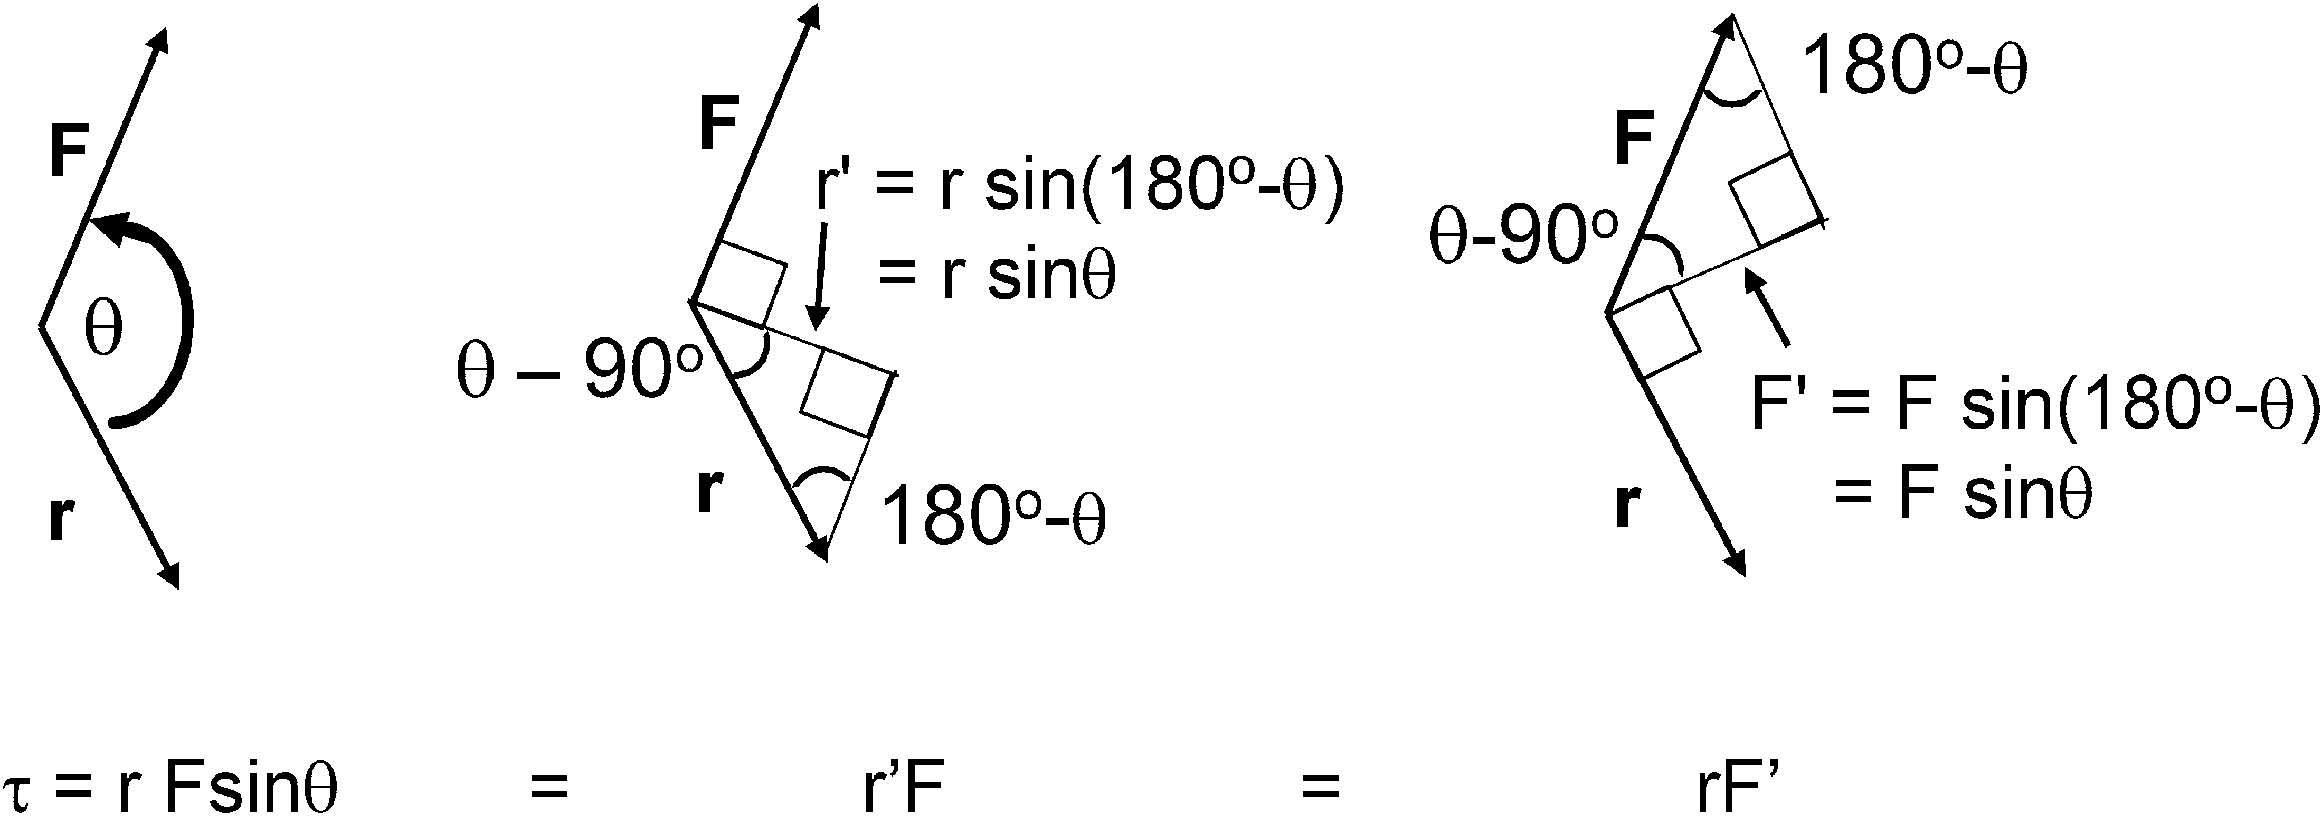
\includegraphics[width=0.7\textwidth]{23.png}
  \caption{Determinación de torques a partir del uso de las componentes de los vectores de desplazamiento y de fuerza que son normales a los vectores de fuerza y desplazamiento, respectivamente.}
  \label{fig:23}
\end{figure}



En el movimiento lineal, una fuerza $\vec{\mathbf{F}}$ conduce a una aceleración $\vec{\mathbf{a}} = \frac{d^2\vec{\mathbf{r}}}{dt^2}$, lo cual es equivalente a un cambio en la velocidad $\vec{\mathbf{v}} = \frac{d\vec{\mathbf{r}}}{dt}$ (cuya magnitud es la rapidez $v$) o al momentum $\vec{\mathbf{p}} = m\vec{\mathbf{v}}$, por
\begin{equation}
\vec{\mathbf{F}} = m\vec{\mathbf{a}} = m\frac{d\vec{\mathbf{v}}}{dt} = \frac{d\vec{\mathbf{p}}}{dt},
\label{eq:2.6}
\end{equation}
donde $m$ es la masa del objeto. De manera similar, un torque $\vec{\boldsymbol{\tau}}$ conduce a un cambio análogo en el ángulo $\theta$ y en la frecuencia angular $\Omega = \frac{d\theta}{dt}$, y en el momento angular orbital $\vec{\mathbf{L}}$
\begin{equation}
\vec{\boldsymbol{\tau}} = I\frac{d\vec{\boldsymbol{\Omega}}}{dt} = \frac{d\vec{\mathbf{L}}}{dt},
\label{eq:2.7}
\end{equation}
donde $I$ es el momento de inercia y $\vec{\mathbf{L}} = I\vec{\boldsymbol{\Omega}}$. En situaciones estáticas, la suma de las fuerzas y los torques sobre el objeto es cero, por lo que el lado derecho de (2.7) es igual a cero. Por cierto, lo que estamos definiendo como torques de hecho se llaman comúnmente «torques» en relación con los movimientos rotacionales y de torsión de los objetos, como en este capítulo y en el Cap. 3, pero en su lugar se llaman «momentos» en relación con la flexión de los objetos, como en el Cap. 4.

\section{Estática: movimiento en un plano y palancas}

Muchos problemas involucran movimiento en un plano, por ejemplo, el plano $x\text{--}y$, para el cual $z$ es una constante. Por ejemplo, el movimiento de las rodillas y los codos es en un plano. Algunos problemas que involucran el movimiento de la pierna alrededor de la cadera pueden tratarse en estas dos dimensiones. Las seis ecuaciones en (2.1) y (2.2) se reducen entonces a tres ecuaciones:
\begin{align}
\sum F_x &= 0, \nonumber \\
\sum F_y &= 0, \nonumber \\
\sum \tau_z &= 0.
\label{eq:2.8}
\end{align}
(Adoptaremos este sistema de coordenadas $x y z$ porque se usa convencionalmente en problemas bidimensionales, a pesar de que difiere de la convención del sistema de coordenadas que adoptamos para el cuerpo en la Fig. 1.1).



\begin{SCfigure}[0.5][htbp]

  \centering
  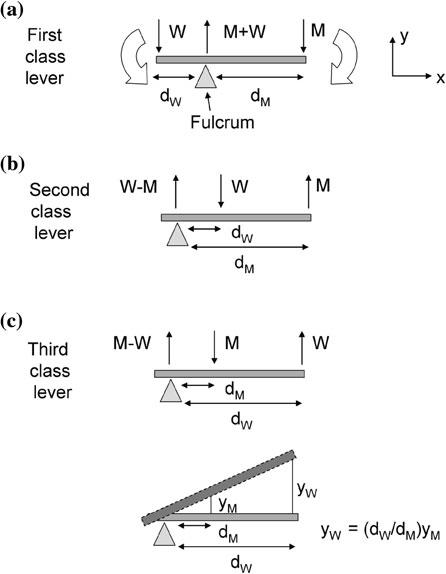
\includegraphics[width=0.5\textwidth]{24.png}
  \caption{Tres tipos de palancas: \textbf{a} de primera clase, \textbf{b} de segunda clase y \textbf{c} de tercera clase. El gran aumento en la distancia que se mueve el peso con respecto al cambio en la longitud del músculo en la palanca de tercera clase también se observa en la parte \textbf{(c)}.}
  \label{fig:24}
\end{SCfigure}

Estos tipos de problemas se pueden clasificar como uno de los tres tipos de palancas (Fig. 2.4). Existen ejemplos en el cuerpo de cada uno. Se pueden describir por cómo un peso $W$ y una fuerza $M$, proporcionada por un músculo, actúan sobre un objeto sólido, por ejemplo, un hueso que descansa sobre un punto de apoyo (fulcro); esto representa una articulación. El peso puede incluir el de partes del cuerpo así como pesos externos. El peso y el músculo actúan a distancias $d_W$ y $d_M$ de la articulación. Para cada tipo de palanca, el torque total es cero cuando
\begin{equation}
M d_M = W d_W,
\label{eq:2.9}
\end{equation}
por lo que
\begin{equation}
M = \frac{d_W}{d_M} W.
\label{eq:2.10}
\end{equation}
Las direcciones relativas de las fuerzas y las distancias relativas de las fuerzas del peso y del músculo con respecto a la articulación son diferentes para cada tipo de palanca.

En una palanca de primera clase, el peso y el músculo actúan en lados opuestos del fulcro y están en la misma dirección (Fig. 2.4a). Este es el tipo de palanca menos común en el cuerpo. Utilizando el sistema de coordenadas $x$, $y$ mostrado, claramente no hay fuerzas en la dirección $x$, por lo que la primera ecuación en (2.8) se satisface automáticamente. Dado que el peso y el músculo actúan en la misma dirección ---hacia abajo---, el balance de fuerzas en la dirección $y$ requiere que el fulcro proporcione una fuerza hacia arriba de $W + M$. El equilibrio de torques en la dirección $z$ requiere la elección de un eje $z$. Se puede elegir cualquier eje normal al plano $xy$. El más simple es un eje en el fulcro. El peso proporciona un torque de $W d_W$, mientras que el músculo proporciona un torque de $-M d_M$. Los signos son consistentes con la discusión anterior. El fulcro no proporciona torque sobre este eje porque la distancia desde el fulcro al eje es cero. Por lo tanto,
\begin{equation}
\tau_z = W d_W - M d_M = 0.
\label{eq:2.11}
\end{equation}
Esto conduce a (2.9), que indica qué tan grande debe ser la fuerza muscular para mantener el equilibrio. Si el músculo no puede proporcionar una fuerza de esta magnitud, no puede haber una condición estática. (Ejemplo: La bola de plomo es demasiado pesada para sostenerla). Si el músculo proporciona más que esta fuerza, hay movimiento intencionado. (Ejemplo: Se está lanzando la pelota de béisbol, como veremos más adelante). En estos dos casos, $\tau_z$ en (2.11) no es cero.

Puede parecer que hicimos trampa al elegir el eje en el fulcro. En realidad, podríamos haber elegido el eje en cualquier parte del plano $xy$. Para demostrarlo, elijamos el eje en cualquier lugar a lo largo del hueso, por ejemplo, a una distancia $x$ a la derecha del peso (Fig. 2.5). Los torques proporcionados por el peso, el fulcro y el músculo son ahora $W x$, $(W + M)(d_W - x)$ y $-M(d_W + d_M - x)$, respectivamente. El equilibrio requiere
\begin{equation}
\tau_z = W x + (W + M)(d_W - x) - M(d_W + d_M - x) = 0,
\label{eq:2.12}
\end{equation}
lo cual se reduce nuevamente a (2.11).

\begin{figure}[htbp]

  \centering
  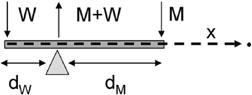
\includegraphics[width=0.7\textwidth]{25.png}
  \caption{Desplazamiento del eje para calcular los torques a la derecha del peso por una distancia $x$, como se muestra para una palanca de primera clase. Para el eje elegido en el fulcro, $x = d_W$. El eje se puede desplazar lateralmente a cualquier lugar, a la izquierda o a la derecha (como se muestra) de la palanca, por encima o por debajo de ella, o dentro de ella.}
  \label{fig:25}
\end{figure}



Un tipo de palanca de primera clase es un balancín o subibaja. Un segundo tipo es la cabeza sobre la columna vertebral, donde el peso de la cabeza se equilibra mediante la fuerza efectiva hacia abajo de los músculos (Fig. 2.6a). En un tercer ejemplo, el tríceps braquial tira del cúbito alrededor del pivote del codo, equilibrado por las fuerzas sobre el antebrazo. Con el brazo superior hacia abajo, el tríceps braquial puede equilibrar una fuerza hacia arriba que empuja la mano hacia arriba (Fig. 2.6b). (Con el brazo superior apuntando hacia arriba, el tríceps braquial también puede equilibrar la mano que sostiene un peso). Debido a que aquí $d_M \ll d_W$, la fuerza que el tríceps braquial necesita ejercer es mucho mayor que las fuerzas ejercidas en la mano.

En una palanca de segunda clase, el músculo y el peso actúan sobre el mismo lado del fulcro, y el peso está más cerca del fulcro, por lo que $M < W$ (Fig. 2.4b). La palanca de segunda clase tiene una ventaja mecánica, lo que significa que la ventaja mecánica, definida como $W/M = d_M/d_W$, es $> 1$. Este tipo de palanca es el segundo más común en el cuerpo. Un ejemplo es pararse de puntillas: la rotación del pie alrededor de los dedos (el fulcro), que sería causada por el peso del pie, se equilibra mediante la fuerza muscular transmitida por el tendón de Aquiles (Fig. 2.6c). Otro ejemplo es empujar hacia abajo con el tríceps braquial.

\begin{SCfigure}[0.5][htbp]

  \centering
  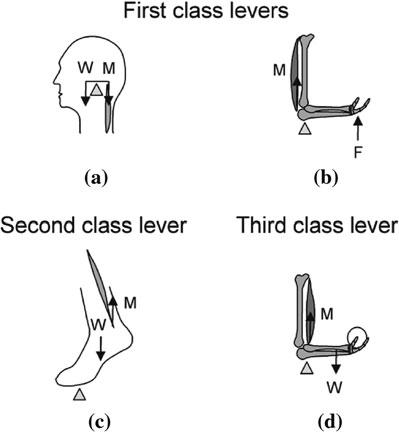
\includegraphics[width=0.55\textwidth]{26.png}
  \caption{Ejemplos de palancas de primera (\textbf{a}, \textbf{b}), segunda (\textbf{c}) y tercera (\textbf{d}) clase en el cuerpo.}
  \label{fig:26}
\end{SCfigure}



En las palancas de tercera clase, el músculo y el peso están nuevamente en el mismo lado del fulcro, pero ahora el músculo está más cerca del fulcro que el peso (Fig. 2.4c). Este es el ejemplo más común en el cuerpo. Debido a que a menudo $d_M \ll d_W$, vemos que $M = (d_W/d_M)W \gg W$. Esta disposición significa que los músculos deben ejercer fuerzas muy grandes debido a esta amplificación de $d_W/d_M$, lo que parece ser una gran desventaja (y es literalmente una desventaja mecánica). Sin embargo, se gana algo más en este compromiso de diseño. Como se ve en la Fig. 2.4c, cuando el hueso rota un ángulo dado, causando un desplazamiento vertical $y_M$ en el músculo, hay una amplificación de la distancia recorrida en la posición del peso por $d_W/d_M$. Como veremos en el Cap. 5, los músculos pueden contraerse solo una pequeña fracción de su longitud ---lo que equivale a lo sumo a unos pocos centímetros en muchos músculos---. La longitud del bíceps es de unos 25 cm, y la contracción máxima es de $\sim 7\text{--}8$ cm. Con esta amplificación, el peso ahora se puede mover mucho más que esto. Un ejemplo de palanca de tercera clase es el equilibrio del antebrazo por el bíceps braquial insertado en el radio (Fig. 2.6d). Otro es sostener un peso con un brazo extendido.

\section{Estática en el cuerpo}

Examinaremos las fuerzas planares en el equilibrio estático del antebrazo, en la cadera y en la espalda. Al analizar el antebrazo, elegiremos modelos sucesivamente más complejos y realistas. Veremos que las fuerzas en la cadera y en la espalda son bastante grandes, mucho más de lo que uno esperaría, y esto explica por qué las personas a menudo tienen problemas en estas partes del cuerpo, problemas que pueden conducir a reemplazos de cadera y dolor lumbar de por vida \cite{1, 8, 36}. El enfoque para estos problemas es el mismo. Consideramos todos los elementos en un plano y examinamos las fuerzas en las direcciones (según definidas) $x$ e $y$ y el torque en la dirección $z$. Se siguen algunos de los enfoques de \cite{3, 28}.

\subsection{El antebrazo}

Examinaremos el equilibrio del antebrazo equilibrado por la contracción del bíceps braquial insertado en el hueso largo del antebrazo llamado radio; esta es una continuación de la discusión sobre las palancas de tercera clase. Los huesos relevantes se muestran en las Figs. 2.7 y 2.8. En equilibrio, la fuerza del bíceps braquial contrarresta la rotación potencial alrededor de la articulación del codo por el peso sostenido en la mano (Fig. 2.9a). Examinaremos este ejemplo para diferentes modelos, utilizando la Fig. 1.15 y las Tablas 1.6 y 1.7 para proporcionar información antropométrica. El antebrazo tiene una longitud de $0,146 H$ y la longitud de la mano es de $0,108 H$, donde $H$ es la altura del cuerpo, por lo que el peso en la mano está aproximadamente a $(0,146 + 0,108/2)H = 0,2 H$ del pivote. (La bola está en el medio de la mano).

\begin{figure}[htbp]

  \centering
  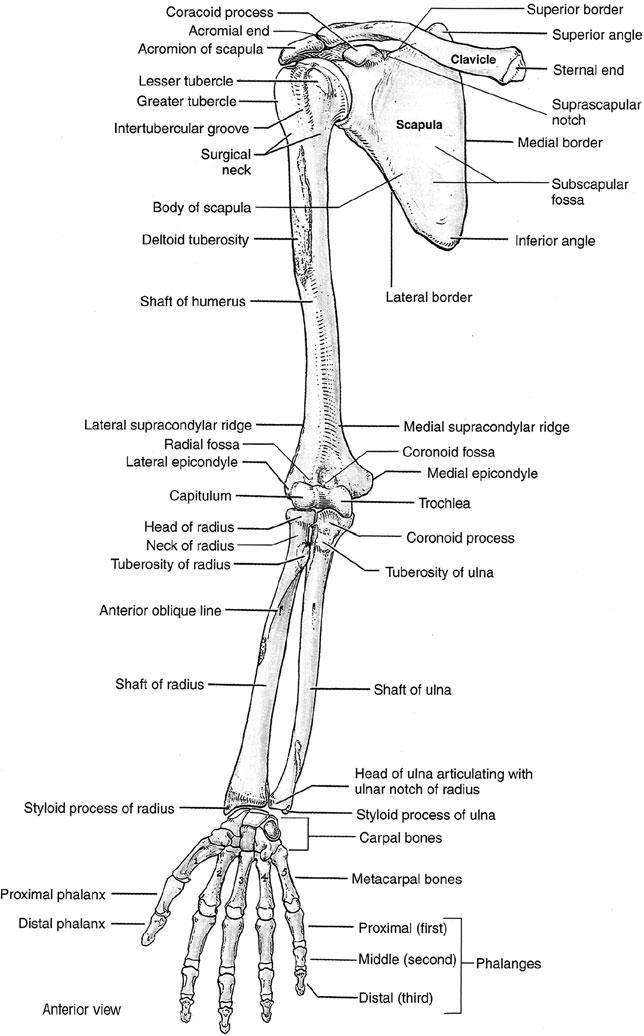
\includegraphics[width=0.55\textwidth]{27.png}
  \caption{Huesos del brazo, vista anterior. (De \cite{20}. Usado con permiso).}
  \label{fig:27}
\end{figure}

\begin{figure}[htbp]

  \centering
  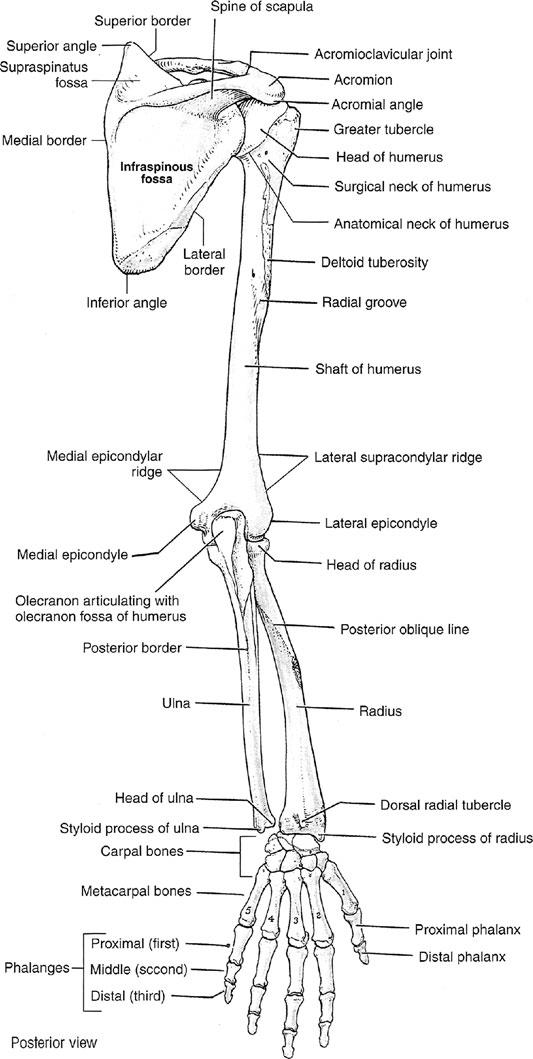
\includegraphics[width=0.55\textwidth]{28.png}
  \caption{Huesos del brazo, vista posterior. (De \cite{20}. Usado con permiso).}
  \label{fig:28}
\end{figure}



\textbf{Caso 1}\\
El bíceps braquial se inserta a unos 4 cm del eje del pivote. Supongamos que hay un peso $W_W$ sostenido en la mano, el cual está a $d_W = 36$ cm del pivote. (Con $H = 180$ cm, $0,2 H = 36$ cm). Por lo tanto, $M = (d_W/d_M)W_W = (36\text{ cm}/4\text{ cm})W_W = 9 W_W$. Así, para un peso de 100 N, el músculo debe proporcionar una fuerza de 900 N para el equilibrio. Aquí N representa la unidad MKS/SI de newtons. Dado que $1\text{ N} \simeq 0,225\text{ lb}$, equivalentemente, un peso de 22 lb se equilibra con 200 lb de fuerza ejercida por el bíceps braquial (Fig. 2.9b).

Hemos hecho varias suposiciones y aproximaciones en este ejemplo sin declararlas explícitamente. Siempre es bueno comenzar con modelos simples. Es igualmente importante comprender exactamente qué suposiciones y aproximaciones se están haciendo. Luego, el modelo se puede hacer más realista. Aquí, hemos asumido que el antebrazo y el brazo superior forman un ángulo de $90^\circ$. También hemos despreciado la masa del antebrazo.

\textbf{Caso 2}\\
Ahora mejoremos el modelo incluyendo el peso del antebrazo $W_F$ (Fig. 2.9c). Esto es $\approx 0,022 W_b$, donde $W_b$ es el peso corporal (Tabla 1.7). Para una persona de 70 kg (700 N, 160 lb), esto es $\approx 15\text{ N}$ (3.4 lb). Podemos tratar el efecto del peso del antebrazo como si estuviera actuando en su centro de masa, el cual está aproximadamente en el medio del antebrazo, a $d_F = 0,146 H/2 = 13$ cm del pivote:

\begin{figure}[htbp]

  \centering
  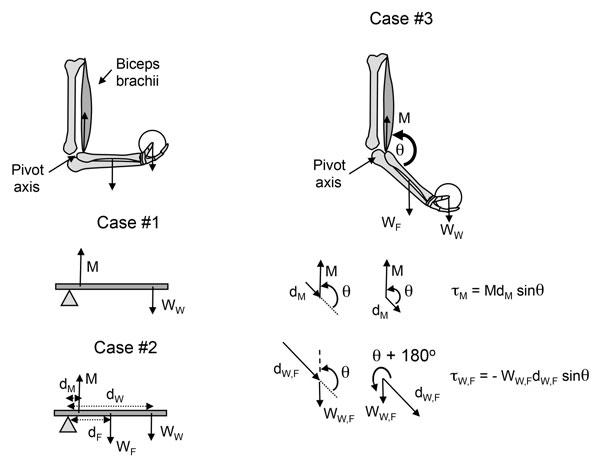
\includegraphics[width=0.75\textwidth]{29.png}
  \caption{\textbf{a} Peso sostenido en la mano, mostrando los músculos bíceps braquial. \textbf{(b--d)} Fuerzas para el equilibrio de un peso sostenido en la mano para los Casos 1--3.}
  \label{fig:29}
\end{figure}


\begin{equation}
\tau_z = M d_M - W_W d_W - W_F d_F = 0
\label{eq:2.13}
\end{equation}
\begin{equation}
M d_M = W_W d_W + W_F d_F
\label{eq:2.14}
\end{equation}
\begin{equation}
M = \frac{d_W}{d_M} W_W + \frac{d_F}{d_M} W_F.
\label{eq:2.15}
\end{equation}
La relación $d_F/d_M$ ($= 13\text{ cm}/4\text{ cm}$), por lo que ahora $M = 9 W_W + 3,25 W_F$ y la fuerza muscular requerida para mantener el equilibrio ha aumentado a $900\text{ N} + (3,25) (15\text{ N}) = 950\text{ N}$ (210 lb).

\textbf{Caso 3}\\
¿Qué pasa si ya no asumimos que el antebrazo y el brazo superior forman un ángulo de $90^\circ$? Mantengamos el brazo superior vertical y dejemos que el antebrazo forme un ángulo $\theta$, el cual puede variar en un rango de más de $142^\circ$ (Tabla 1.10). La fuerza debida al músculo es entonces todavía vertical, y aquellas debidas a los pesos del antebrazo y de la bola son, por supuesto, hacia abajo. A partir de la Fig. 2.9d vemos que el torque causado por cada una de estas tres fuerzas se multiplica por $\sin \theta$. Ahora
\begin{equation}
\tau_z = M d_M \sin \theta - W_W d_W \sin \theta - W_F d_F \sin \theta = 0
\label{eq:2.16}
\end{equation}
y llegamos al mismo resultado de que
\begin{equation}
M d_M = W_W d_W + W_F d_F.
\label{eq:2.17}
\end{equation}

En realidad, hicimos suposiciones adicionales en este ejemplo que volveremos a examinar más adelante. La distancia desde el pivote donde el bíceps braquial se inserta en el radio realmente cambia con $\theta$ (Fig. 3.46). Además, aunque este análisis sugiere que la fuerza muscular $M$ requerida para el equilibrio es la misma para todos los ángulos, hay una sutileza en este resultado. La ecuación (2.16) da la fuerza muscular necesaria para mantener el equilibrio. Como veremos en el Cap. 5, los músculos pueden ejercer fuerzas hasta un valor máximo. Si se puede lograr la fuerza $M$ de (2.17), entonces puede haber equilibrio; si no se puede, entonces no se puede lograr la condición estática. La fuerza máxima que un músculo puede ejercer depende de su longitud, la cual, a partir de la Fig. 2.9, es claramente una función de $\theta$. Por lo tanto, la fuerza $M$ en (2.17) puede ser alcanzable en algunos ángulos (más cercanos a $90^\circ$, donde resulta que la fuerza máxima es mayor) y no en otros.

\textbf{Caso 4}\\
El bíceps braquial no es el único músculo utilizado para flexionar el codo. ¿Qué sucede si también incluimos las contribuciones de estos otros músculos? La Fig. 2.10 muestra que el bíceps braquial, el braquial y el braquiorradial contribuyen a esta flexión. Asumiendo que $\theta = 90^\circ$ (lo cual puede no ser una buena suposición para cada músculo), la ecuación (2.13) se modifica a
\begin{equation}
\tau_z = M_1 d_{M1} + M_2 d_{M2} + M_3 d_{M3} - W_W d_W - W_F d_F = 0
\label{eq:2.18}
\end{equation}
\begin{equation}
M_1 d_{M1} + M_2 d_{M2} + M_3 d_{M3} = W_W d_W + W_F d_F
\label{eq:2.19}
\end{equation}

\begin{figure}[htbp]

  \centering
  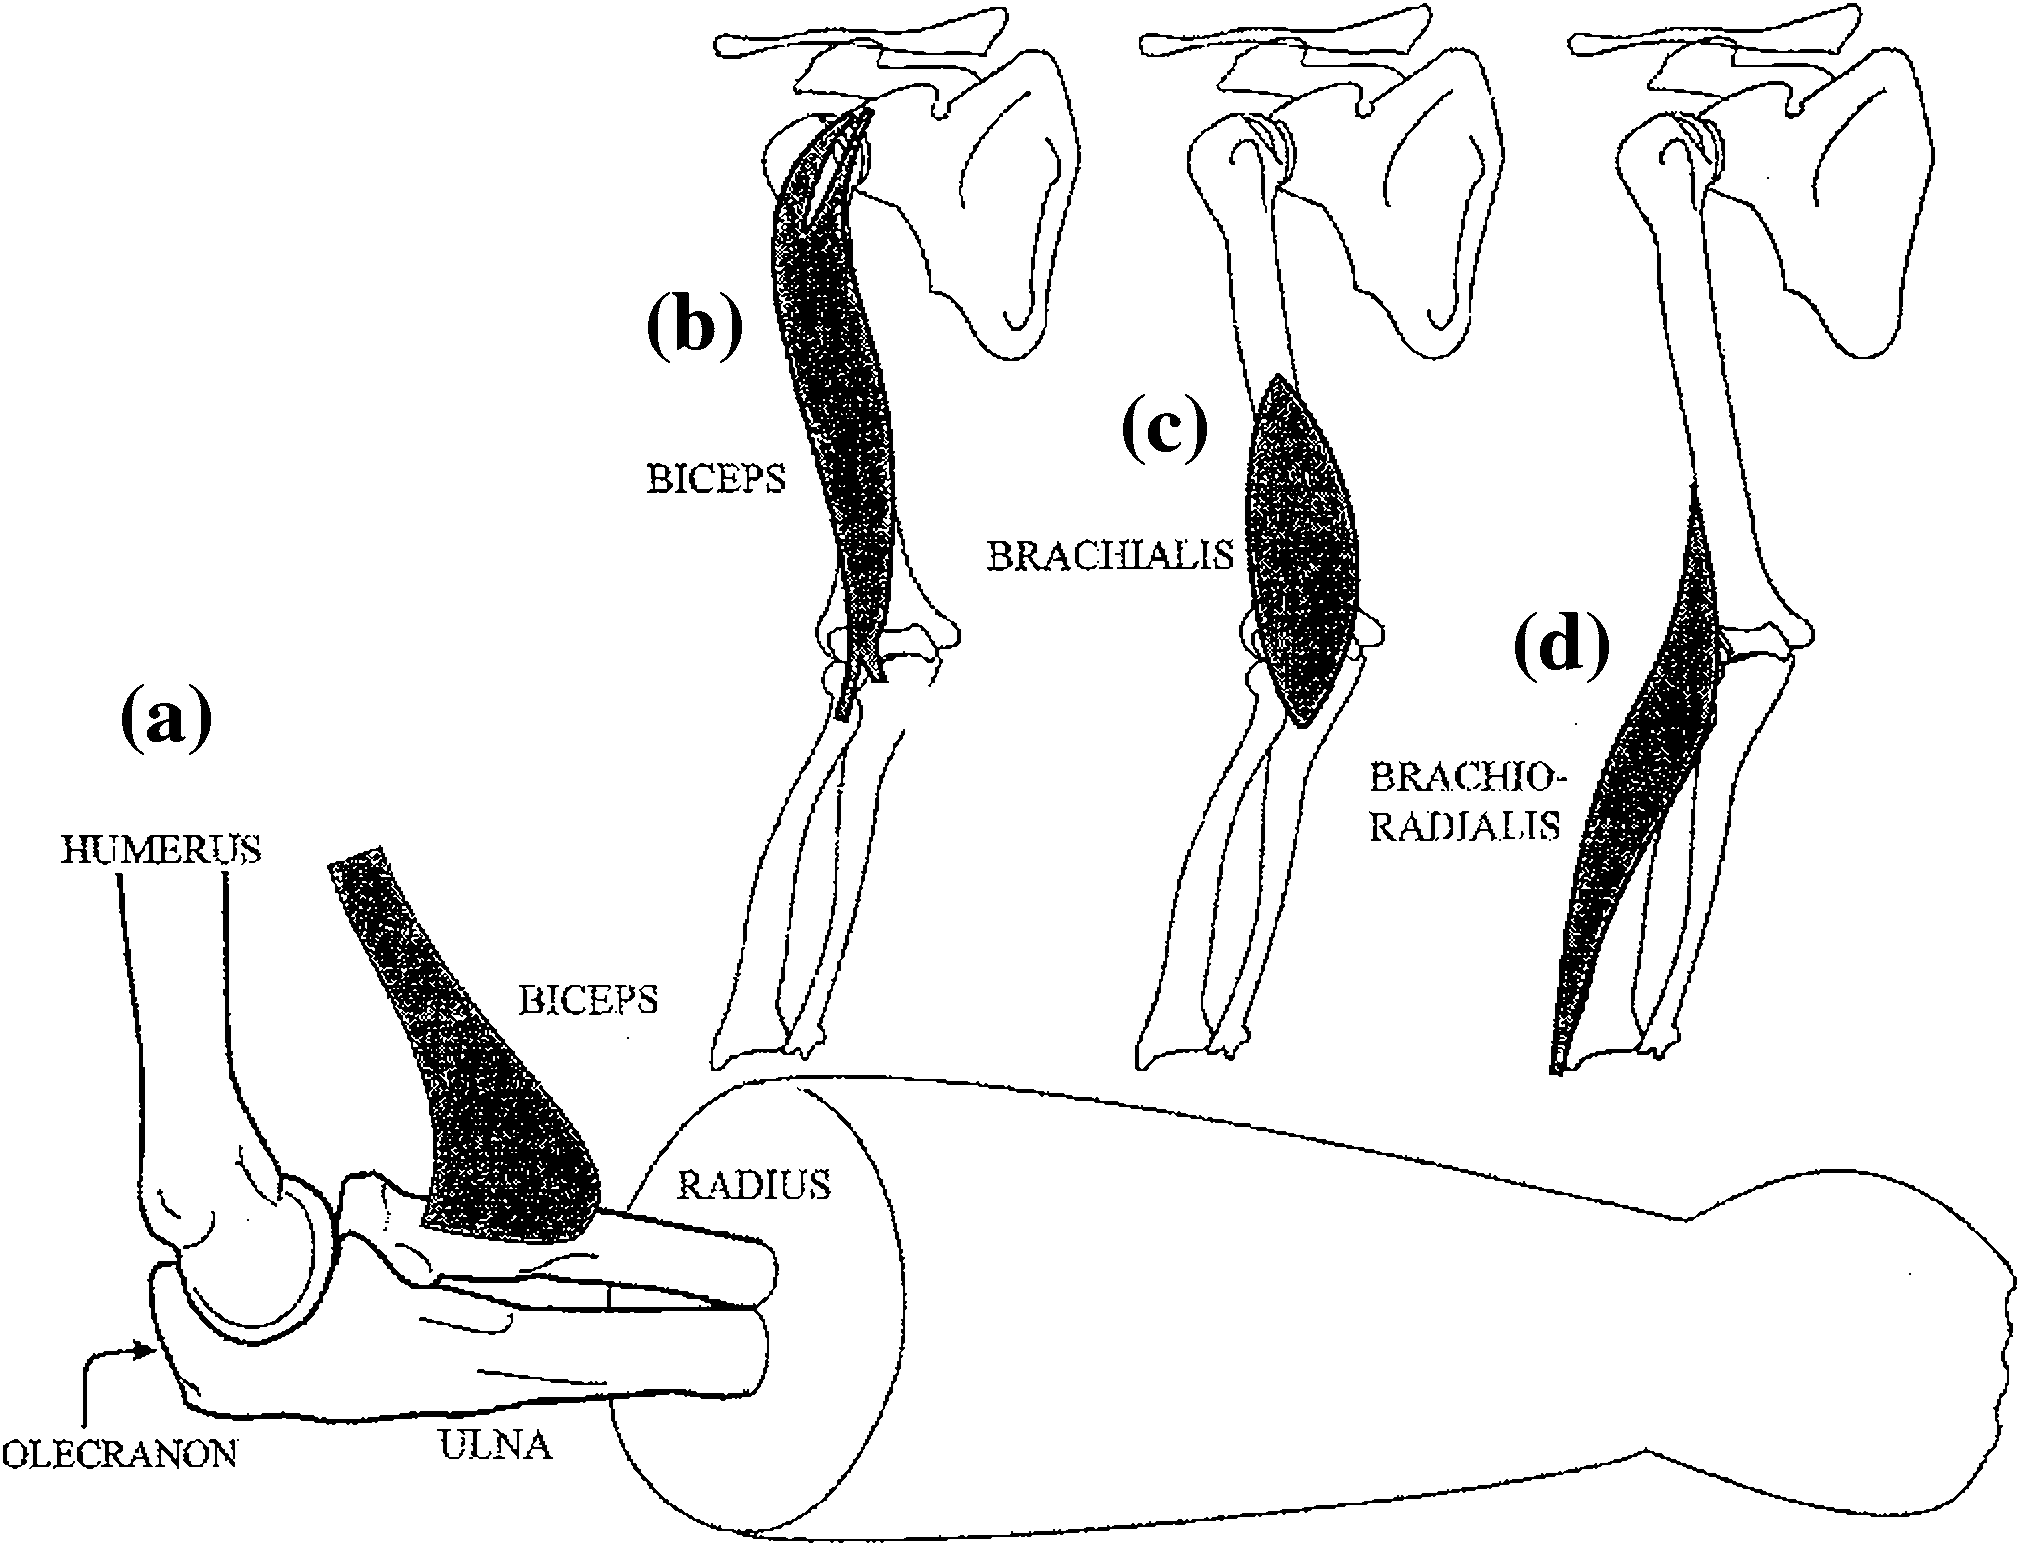
\includegraphics[width=0.75\textwidth]{210.png}
  \caption{Bosquejo de la articulación del codo para analizar la estática del antebrazo para el Caso 4, con los tres músculos, el bíceps (braquial), el braquial y el braquiorradial, mostrados en \textbf{(b--d)}. (De \cite{18}).}
  \label{fig:210}
\end{figure}


donde $M_1$, $M_2$ y $M_3$ representan las fuerzas ejercidas por los tres músculos $M_i$, respectivamente. Si las áreas de sección transversal fisiológica de los tres músculos son $A_1$, $A_2$ y $A_3$, respectivamente (que normalmente llamamos ASTF o PCA, por sus siglas en inglés, \textit{physiological cross-sectional areas}), y se puede asumir que la fuerza muscular para cada uno es proporcional a este área (lo cual es una suposición bastante buena), entonces $M_i = k A_i$, para $i = 1, 2, 3$. (Veremos que esta es una buena suposición con $k$ alcanzando un máximo de $\sim 40\text{ N/cm}^2$ aproximadamente). Por lo tanto,
\begin{equation}
k A_1 d_{M1} + k A_2 d_{M2} + k A_3 d_{M3} = W_W d_W + W_F d_F
\label{eq:2.20}
\end{equation}
\begin{equation}
k = \frac{W_W d_W + W_F d_F}{A_1 d_{M1} + A_2 d_{M2} + A_3 d_{M3}}
\label{eq:2.21}
\end{equation}
\begin{equation}
M_1 = k A_1 = A_1 \frac{W_W d_W + W_F d_F}{A_1 d_{M1} + A_2 d_{M2} + A_3 d_{M3}}
\label{eq:2.22}
\end{equation}
\begin{equation}
M_2 = k A_2 = A_2 \frac{W_W d_W + W_F d_F}{A_1 d_{M1} + A_2 d_{M2} + A_3 d_{M3}}
\label{eq:2.23}
\end{equation}
\begin{equation}
M_3 = k A_3 = A_3 \frac{W_W d_W + W_F d_F}{A_1 d_{M1} + A_2 d_{M2} + A_3 d_{M3}}.
\label{eq:2.24}
\end{equation}

Utilizando los parámetros de la Tabla 2.1, obtenemos $M_1 = 262\text{ N}$ (bíceps), $M_2 = 399\text{ N}$ (braquial) y $M_3 = 85\text{ N}$ (braquiorradial) cuando generalizamos el Caso 2. Esto se compara con la fuerza $M_1 = 696\text{ N}$ que obtendríamos para el Caso 2 con el bíceps solo, utilizando $d_1 = 4,6$ cm (en lugar de los 4 cm utilizados anteriormente, que conducían a 800 N). La fuerza muscular total es de 746 N, que es mayor que 696 N debido a que el braquial tiene un brazo de momento relativamente pequeño.

La vida es un poco más compleja de lo que sugiere este resultado porque asumimos que $k$ tiene el mismo valor para cada músculo. En realidad, $M_i = k_i A_i$, y todos los valores de $k_i$ no necesitan ser iguales, siempre que $k_i$ sea menor que el máximo que pueden ejercer los músculos. Desafortunadamente, si no se asume que todos los valores de $k_i$ son iguales, no tenemos suficiente información para resolver este problema de manera única tal como se plantea. El cuerpo puede resolver la naturaleza indeterminada de este problema (con más variables que condiciones) minimizando la energía o bien optimizando la distribución de la fuerza (desplazando la carga de un músculo a otro) para descansar músculos específicos, o manteniendo el peso mejor equilibrado (para que no se incline en la mano).

\begin{table}[htbp]
\centering
\caption{Datos para los tres músculos del codo utilizados para la flexión.}
\label{tab:21}
\begin{tabularx}{0.8\textwidth}{l>{\centering\arraybackslash}X>{\centering\arraybackslash}X}
\toprule
\textbf{Músculo} & \textbf{Brazo de momento $d_i$ (cm)} & \textbf{Sección transversal fisiológica (PCA) ($\text{cm}^2$)} \\
\midrule
Bíceps (músculo 1) & 4,6 & 4,6 \\
Braquial (músculo 2) & 3,4 & 7,0 \\
Braquiorradial (músculo 3) & 7,5 & 1,5 \\
\bottomrule
\end{tabularx}
\begin{flushleft}
    \small Utilizando datos de \cite{18, 39}
\end{flushleft}
\end{table}

\subsection{Problemas de cadera}

La cadera (pelvis) no es un solo hueso, sino varios huesos que están fusionados (Figs. 2.11 y 2.12). La pelvis está compuesta por la cintura pélvica y dos partes de la médula espinal (o columna vertebral): el sacro y el coxis. La cintura pélvica a su vez está compuesta por los huesos coxales (o de la cadera) derecho e izquierdo. Cada hueso coxal (cadera) está compuesto por tres huesos: el ilion (en la parte superior = superior), el pubis (en la parte inferior frontal = inferior, anterior) y el isquion (\textit{ischium}, pronunciado «iss-kee-um») (en la parte inferior trasera = inferior, posterior). El acetábulo (\textit{acetabulum}, pronunciado «a-si-tab-yoo-lum») es el área de la fosa (o cavidad) donde se une el fémur de la pierna (Fig. 2.13) («articulación de la cadera»). En realidad, la cabeza del fémur está en esta cavidad y se mantiene allí mediante los músculos unidos al trocánter mayor. Estos músculos se denominan colectivamente músculos abductores de la cadera. (Los músculos abductores de la cadera no son los únicos unidos al trocánter mayor (ver más abajo), pero son los que contribuyen a la fuerza necesaria para la condición de equilibrio en este problema).

Primero determinaremos la fuerza sobre la cabeza del fémur y en los músculos abductores de la cadera mientras el sujeto está parado sobre una pierna, digamos la pierna derecha. Este es en realidad un buen modelo para determinar estas fuerzas durante la marcha lenta. El muslo y la pantorrilla (la parte superior e inferior de la pierna) y el pie se tratan como un cuerpo rígido. Este problema se resuelve en dos pasos. Primero, se analizan las fuerzas en todo el cuerpo y luego la pierna rígida se trata como un cuerpo rígido libre, cuya única interacción con el resto del cuerpo será la fuerza normal de la cadera \cite{3, 27}. Los huesos de la pierna se muestran en las Figs. 2.14 y 2.15.

\begin{SCfigure}[0.5][htbp]

  \centering
  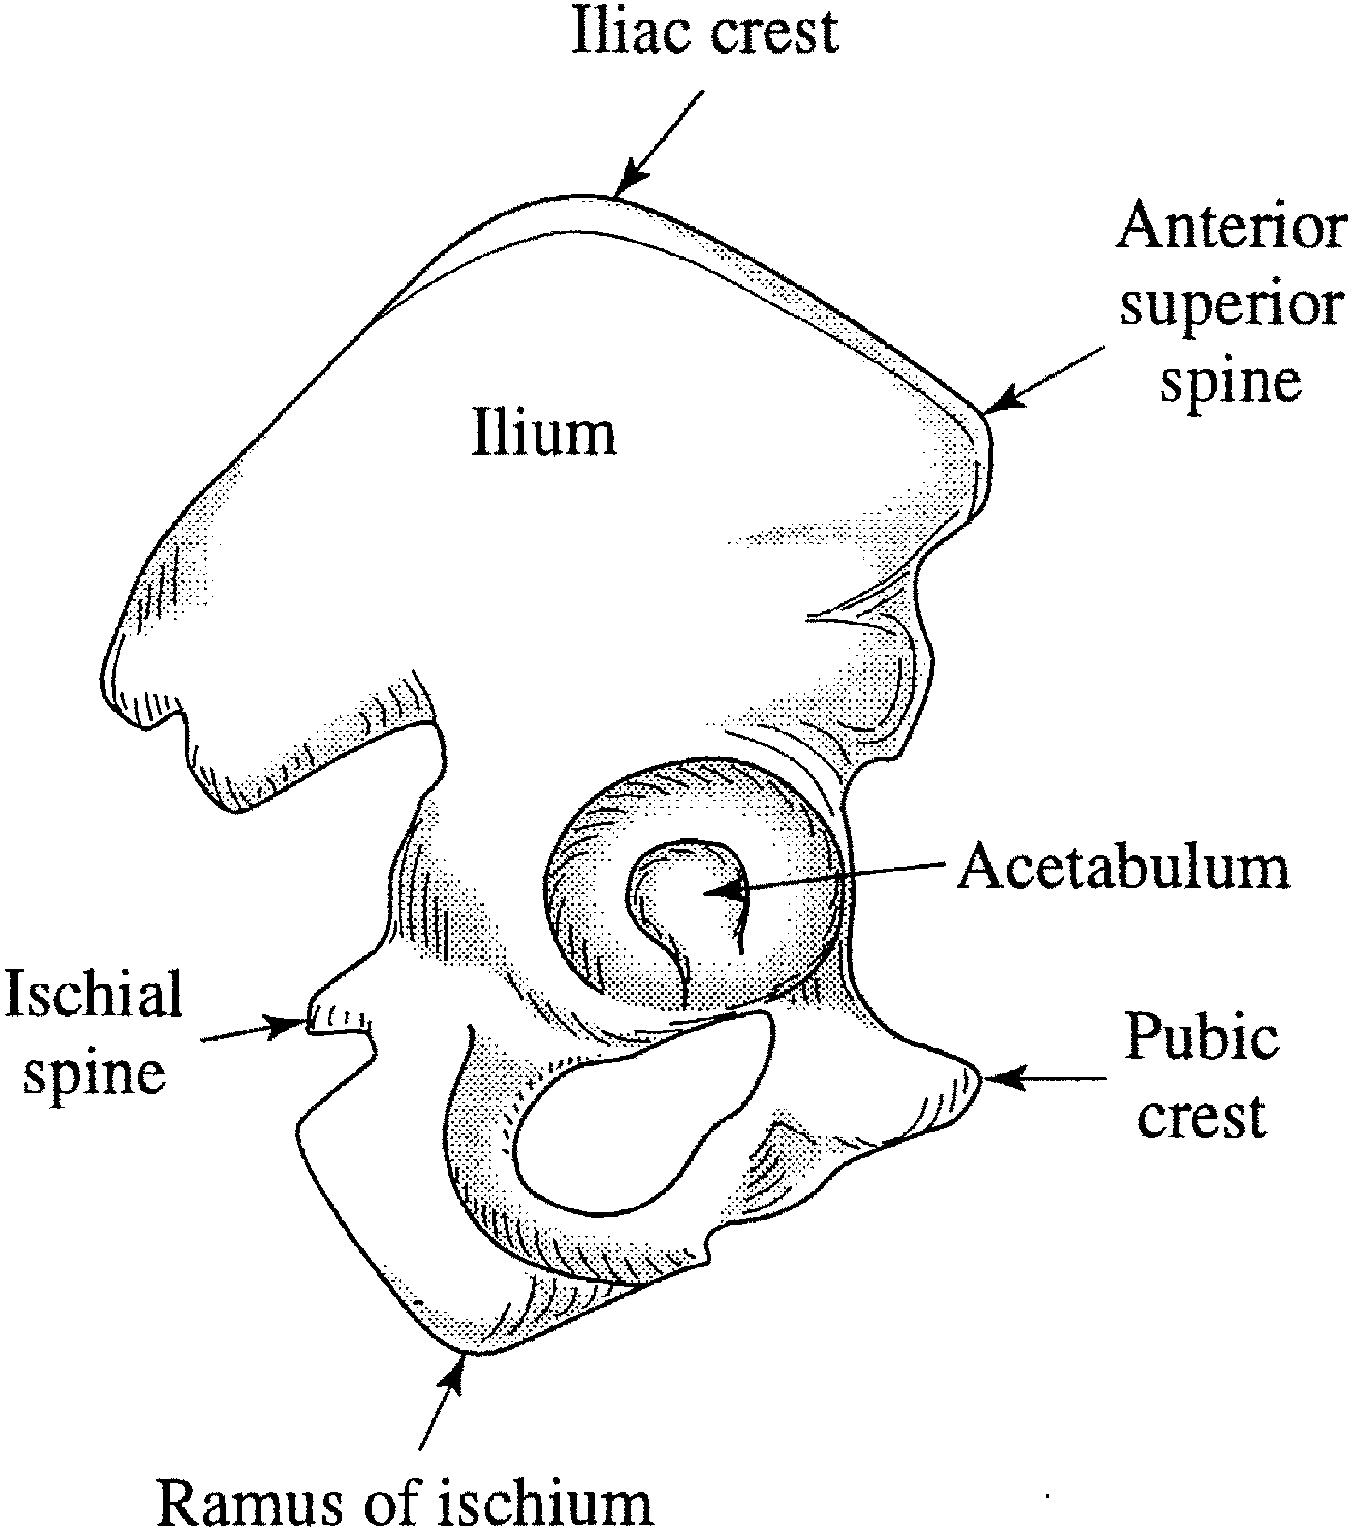
\includegraphics[width=0.5\textwidth]{211.png}
  \caption{Hueso de la cadera derecha en un adulto. (De \cite{3}).}
  \label{fig:211}
\end{SCfigure}

\begin{figure}[htbp]

  \centering
  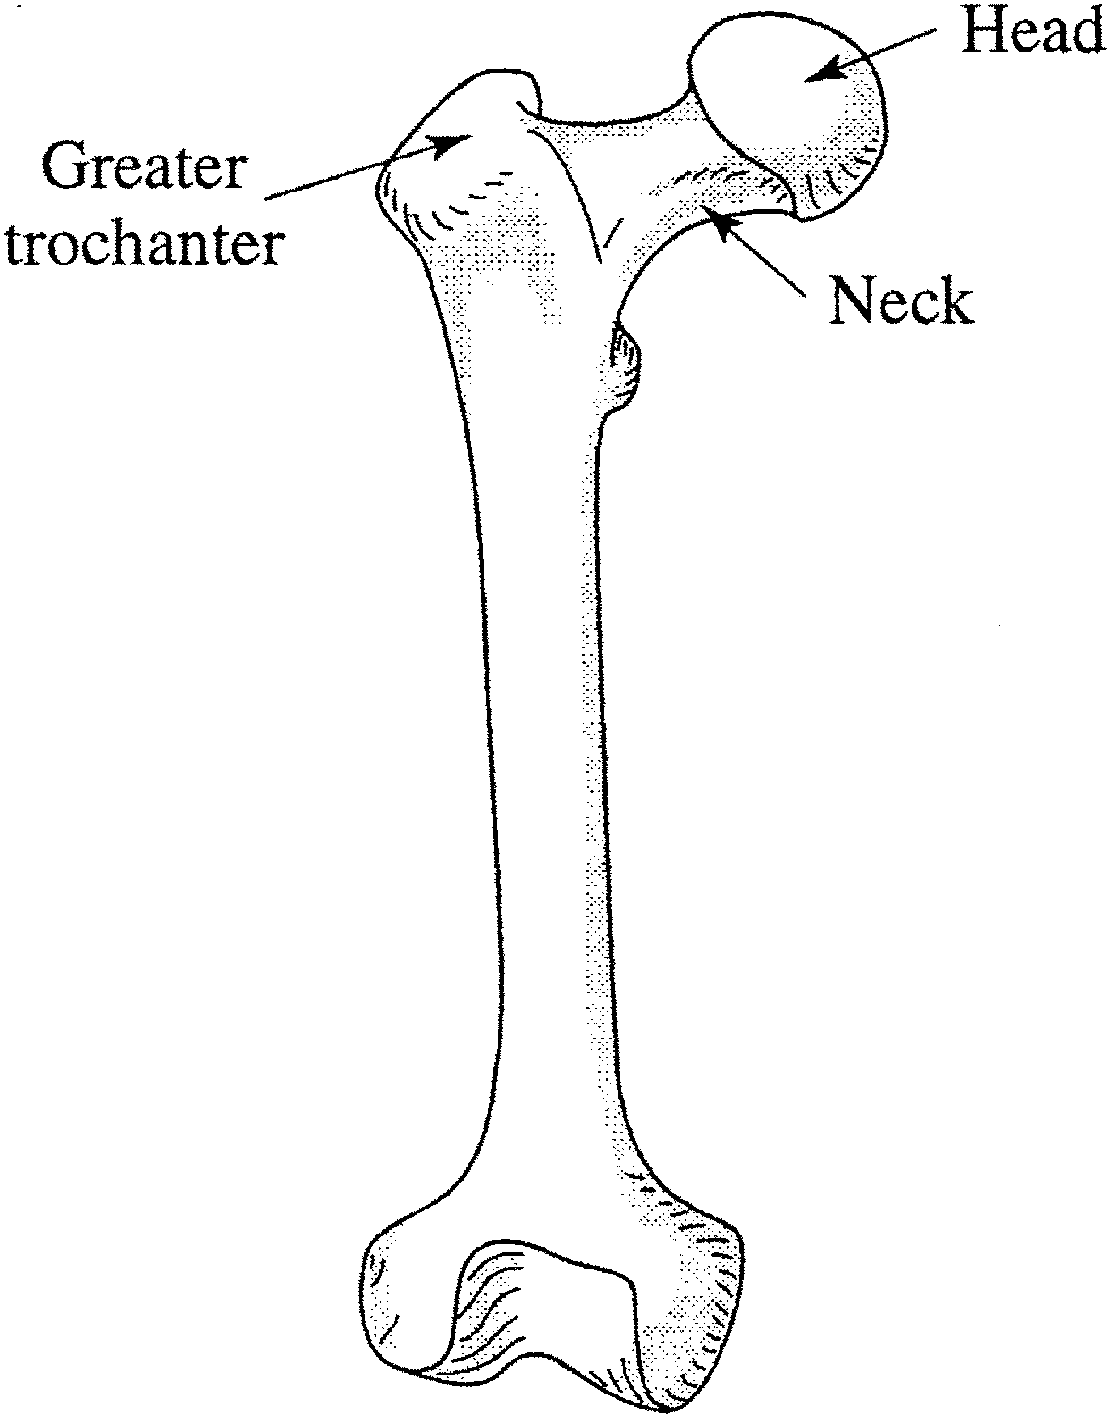
\includegraphics[width=0.55\textwidth]{212.png}
  \caption{Vistas frontal y lateral de la cadera. (De \cite{3}).}
  \label{fig:212}
\end{figure}

\begin{SCfigure}[0.5][htbp]

  \centering
  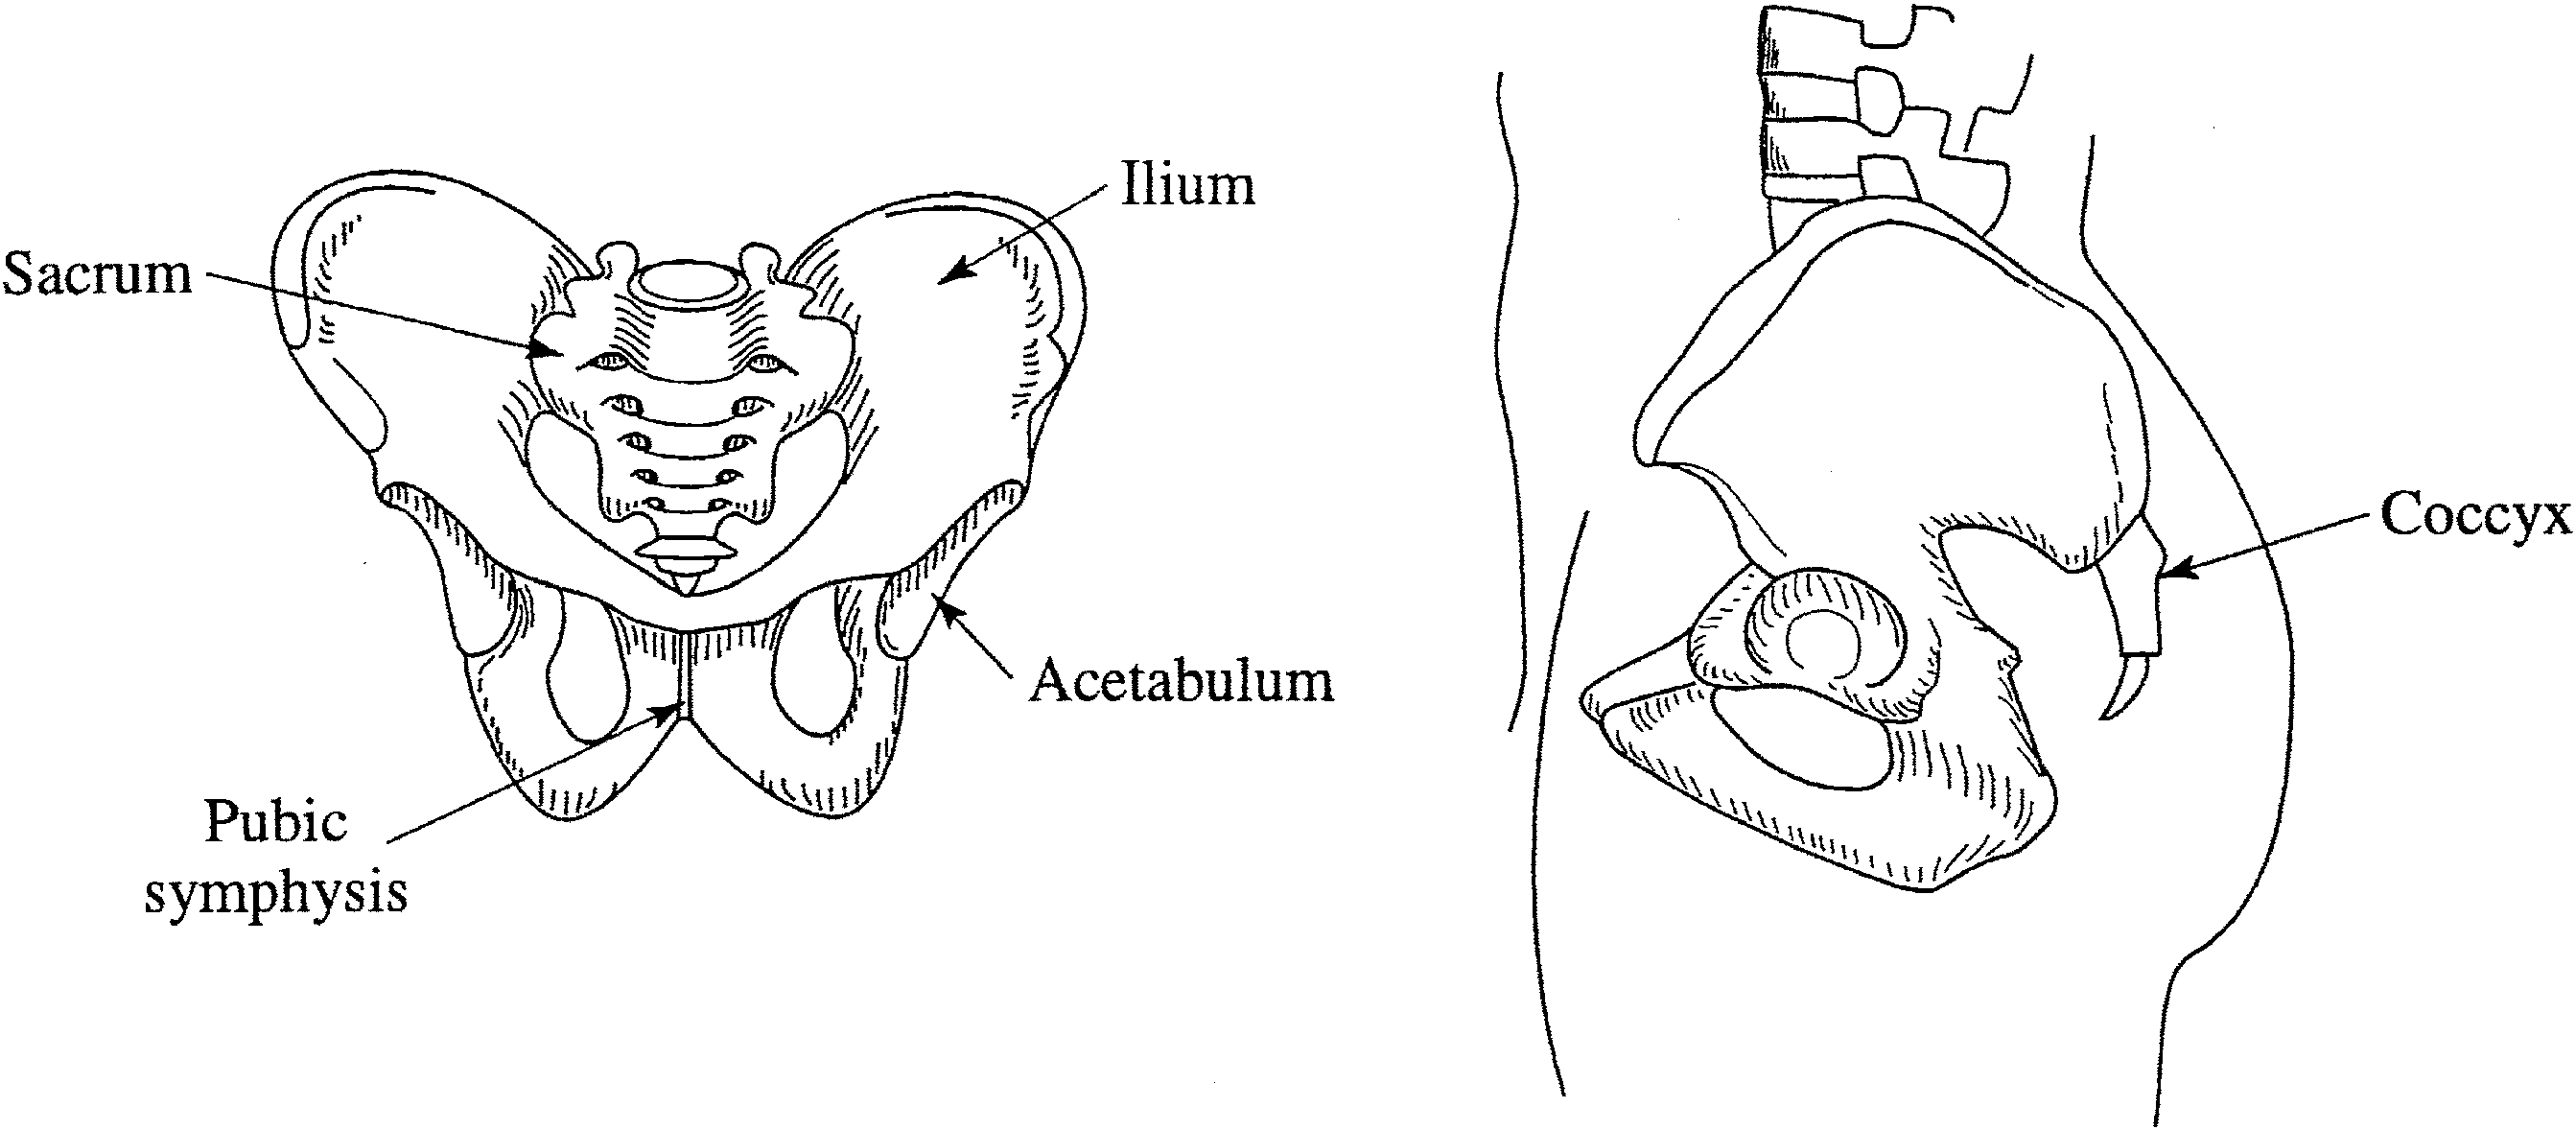
\includegraphics[width=0.55\textwidth]{213.png}
  \caption{Vista anterior del fémur derecho. (De \cite{3}).}
  \label{fig:213}
\end{SCfigure}



\subsubsection{Equilibrio del cuerpo completo}

Hay solo dos fuerzas sobre el cuerpo. El peso corporal $W_b$ actúa hacia abajo, y como si todo se originara en el centro de masa del cuerpo, el cual está en la línea media en la cadera (Fig. 2.16). El pie experimenta una fuerza normal hacia arriba desde el suelo de magnitud $N$. No hay fuerzas en la dirección $x$, y estas dos fuerzas en la dirección $y$ deben equilibrarse en equilibrio, por lo que $N = W_b$. En equilibrio, el cuerpo no puede comenzar a rotar, por lo que los torques son cero. Si elegimos el eje del pivote en el centro de masa, el torque del centro de masa es cero porque el término de distancia (desde el eje hasta el centro de masa) es cero, y el torque de la fuerza normal es cero debido a que la fuerza normal es antiparalela al vector de distancia ($\theta = 180^\circ$). (Usted mismo puede demostrar que el torque total es cero para cualquier otro eje normal al plano $xy$).

\begin{figure}[htbp]

  \centering
  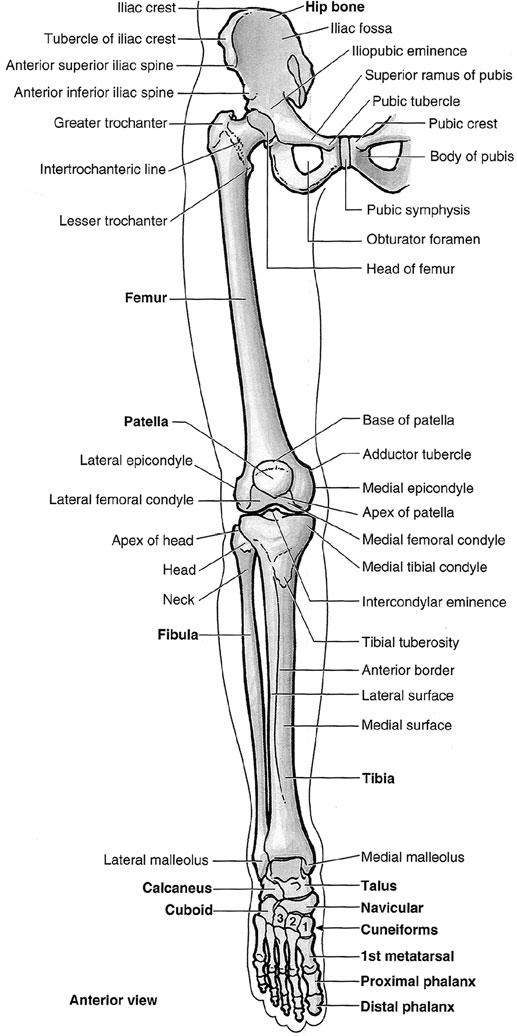
\includegraphics[width=0.55\textwidth]{214.png}
  \caption{Huesos de la pierna y la cadera, vista anterior, con los nombres de los huesos en negrita. (De \cite{21}. Usado con permiso).}
  \label{fig:214}
\end{figure}

\begin{figure}[htbp]

  \centering
  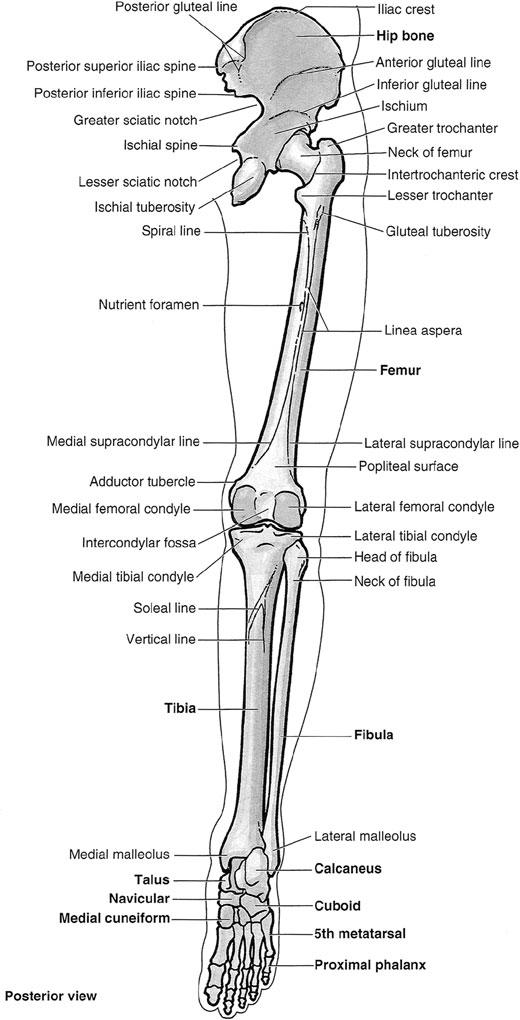
\includegraphics[width=0.55\textwidth]{215.png}
  \caption{Huesos de la pierna y la cadera, vista posterior, con los nombres de los huesos en negrita. (De \cite{21}. Usado con permiso).}
  \label{fig:215}
\end{figure}

\begin{SCfigure}[0.5][htbp]

  \centering
  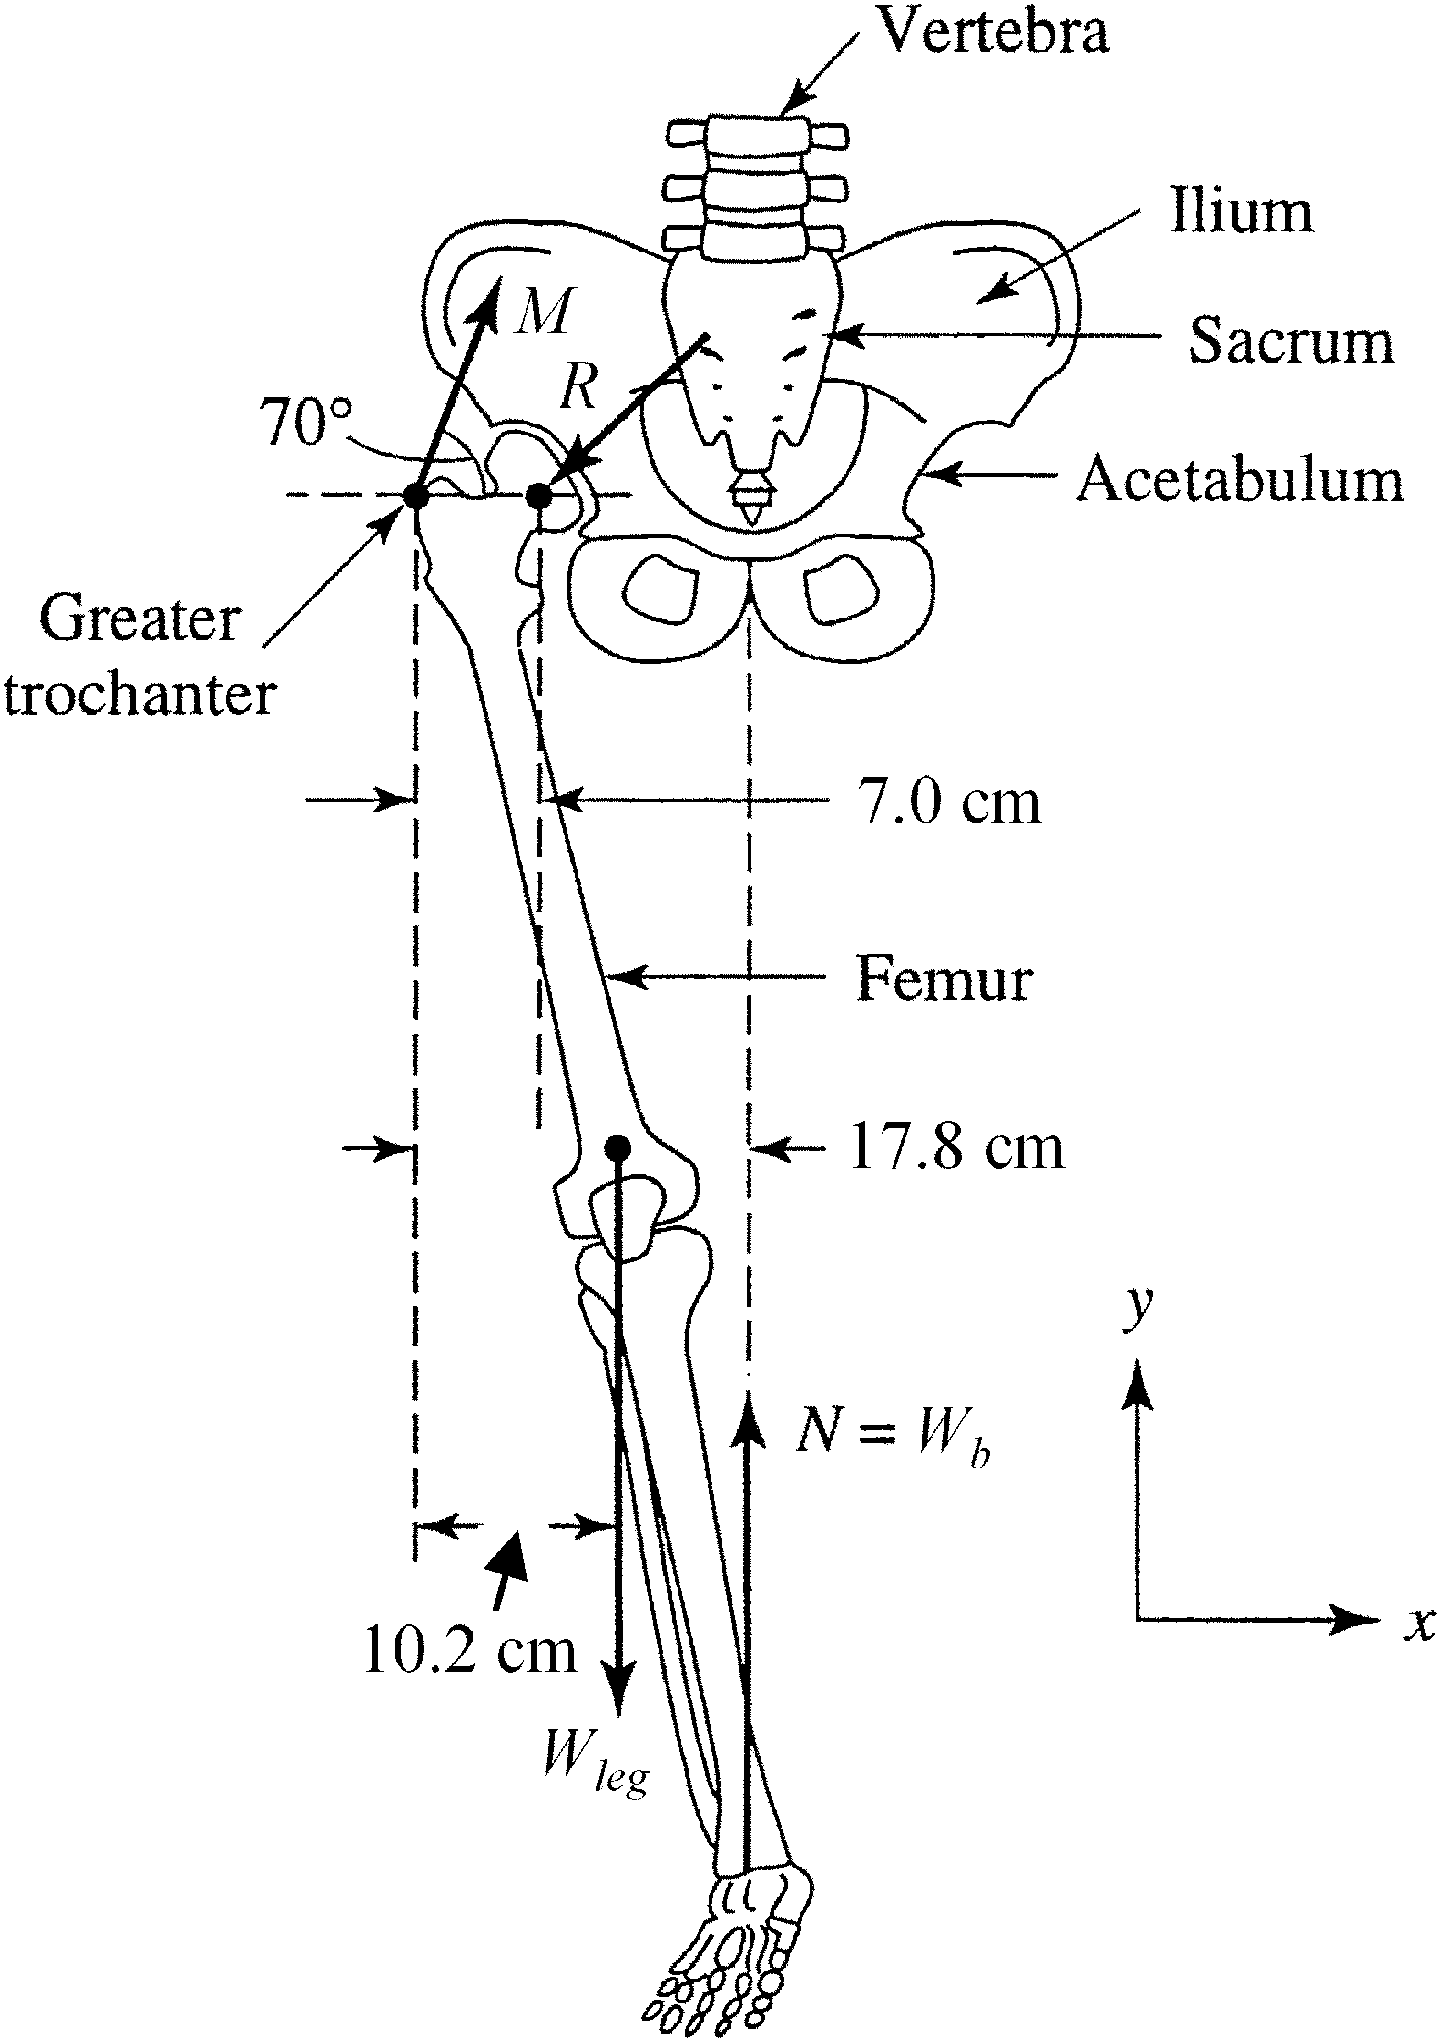
\includegraphics[width=0.5\textwidth]{216.png}
  \caption{Diagrama anatómico de la pierna y la cadera para alguien parado sobre una pierna, o durante la marcha lenta, mostrando las fuerzas sobre ellas y las dimensiones relevantes, incluyendo la fuerza ejercida sobre la cabeza del fémur por el acetábulo $\vec{\mathbf{R}}$ y la fuerza neta ejercida por los músculos abductores de la cadera. (De \cite{3}).}
  \label{fig:216}
\end{SCfigure}



\subsubsection{Equilibrio del componente corporal individual}

Hay cuatro fuerzas externas sobre la pierna (Figs. 2.16 y 2.17):

(a) $N$ es la fuerza normal sobre la pierna desde el suelo, y sabemos que $N = W_b$.

(b) $W_{\text{leg}}$ es el peso de la pierna. La Tabla 1.7 muestra que esto es alrededor de $0,16 W_b$. Actúa como si estuviera aplicado en el centro de masa de la pierna, el cual está aproximadamente a la mitad de la altura de la pierna.

(c) $\vec{\mathbf{R}}$ es la fuerza de reacción sobre la pierna desde la cadera, y es normal a la cavidad de la cadera. Definiremos las componentes $x$ e $y$, $R_x$ y $R_y$, de modo que sean positivas (Fig. 2.17). Equivalentemente, podríamos definir la magnitud de $\vec{\mathbf{R}}$ y el ángulo que forma con la vertical, $\phi$.

\begin{SCfigure}[0.5][htbp]

  \centering
  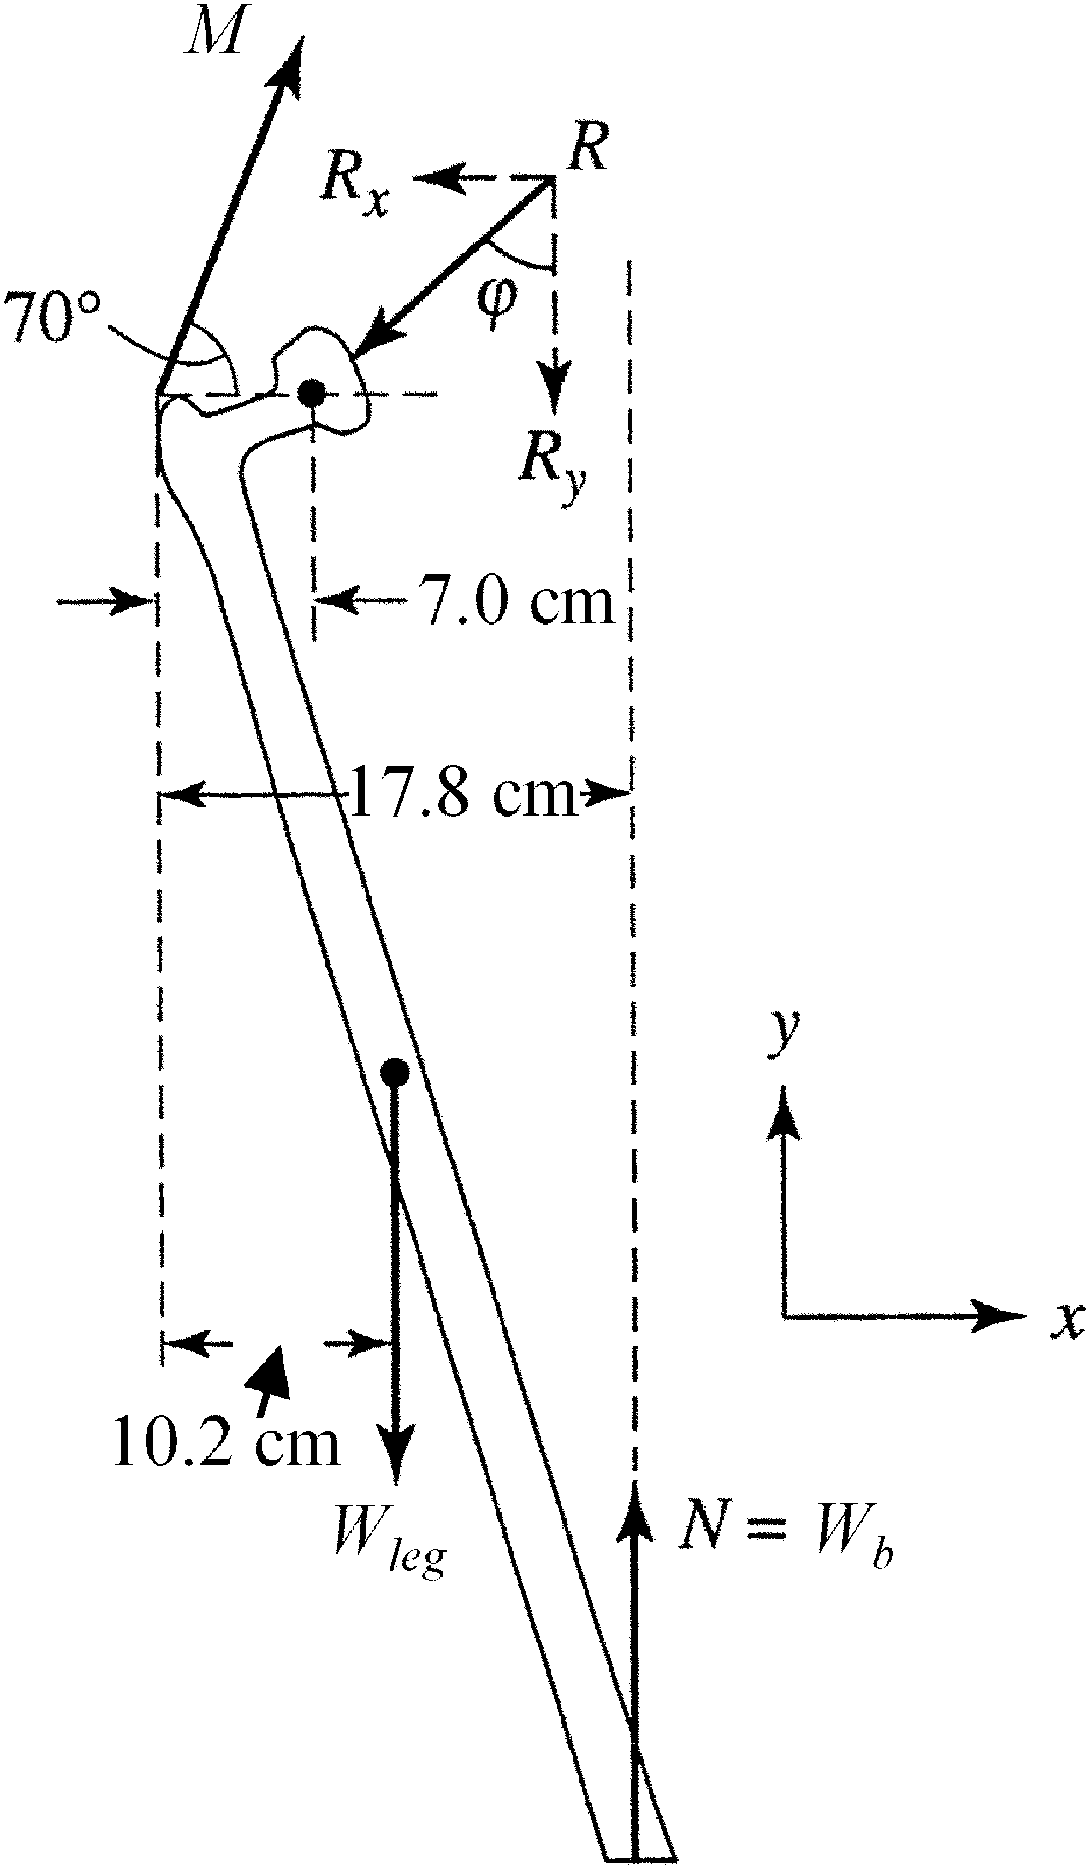
\includegraphics[width=0.5\textwidth]{217.png}
  \caption{Diagrama de fuerzas para una pierna para alguien parado sobre un pie, utilizando la Fig. 2.16. (De \cite{3}).}
  \label{fig:217}
\end{SCfigure}



(d) $\vec{\mathbf{M}}$ es la fuerza (de magnitud $M$) debida a los músculos abductores de la cadera. En realidad, aquí hay tres músculos involucrados: el tensor de la fascia lata (\textit{tensor fascia latae}, pronunciado «fash-ee-uh la-tuh») (ver Fig. 3.3a), el glúteo menor (\textit{gluteus minimus}, pronunciado «gloo-tee-us») (ver Fig. 3.3c) y el glúteo medio (\textit{gluteus medius}) (ver Fig. 3.3a, b). (El músculo glúteo mayor es sobre el que está sentado el autor mientras escribe esto). Estos tres músculos tienen una relación de masa de aproximadamente 1:2:4 y, como veremos, esta es aproximadamente la relación de las fuerzas que cada uno puede ejercer. La estructura del músculo abductor de la cadera que consideramos es un compuesto de los tres músculos. Se ha demostrado que la acción efectiva de este sistema es $\simeq 70^\circ$ con respecto a la horizontal, actuando sobre el trocánter mayor.

Tenemos tres ecuaciones con tres incógnitas: $R_x$, $R_y$ y $M$. Las dos ecuaciones de fuerza son:
\begin{equation}
F_x = M \cos 70^\circ - R_x = 0,
\label{eq:2.25}
\end{equation}
\begin{equation}
F_y = M \sin 70^\circ - R_y - 0,16 W_b + W_b = 0,
\label{eq:2.26}
\end{equation}
donde $W_{\text{leg}}$ ha sido reemplazado por $0,16 W_b$.

Elegiremos el eje de rotación de modo que emane del centro de la cabeza del fémur porque la fuerza de reacción desde el acetábulo pasa por este punto. Esto facilita el análisis, pero, por supuesto, la solución sería la misma si eligiéramos cualquier otro eje paralelo. Las distancias de interés relevantes se muestran en el diagrama (obtenidas de las dimensiones anatómicas y la geometría), según sea necesario para el análisis del torque.

(a) La componente del vector de distancia perpendicular a la fuerza normal ($r'$) es de 10,8 cm, por lo que la fuerza normal causa un torque de $(10,8\text{ cm})W_b$. Este es un torque positivo porque la fuerza normal induce una rotación en sentido antihorario al rededor del eje $z$ elegido (ver Fig. 2.2).

(b) La componente del vector de distancia normal a la fuerza del peso de la pierna es de 3,2 cm y esta fuerza tiende a inducir una rotación en sentido horario, por lo que contribuye con un torque de $-(3,2\text{ cm})W_{\text{leg}} = -(3,2\text{ cm})(0,16 W_b) = -(0,5\text{ cm})W_b$.

(c) Con la elección de este eje, el torque de la fuerza de reacción desde la cadera es cero, porque el vector de distancia y la fuerza normal son antiparalelos.

(d) La componente de la fuerza de los músculos abductores de la cadera normal al vector de distancia horizontal (de magnitud 7,0 cm) es $M \sin 70^\circ$. Dado que esto causa una rotación en sentido horario, el torque es $-(7,0\text{ cm})M \sin 70^\circ$. Así vemos que
\begin{equation}
\tau_z = (10,8\text{ cm})W_b - (3,2\text{ cm})(0,16 W_b) + 0 - (7,0\text{ cm})M \sin 70^\circ = 0,
\label{eq:2.27}
\end{equation}
\begin{equation}
M = \frac{10,8 - 0,5}{7,0 \sin 70^\circ} W_b = 1,57 W_b.
\label{eq:2.28}
\end{equation}

Vemos que el torque proporcionado por los músculos abductores de la cadera es necesario para contrarrestar los torques de la fuerza normal desde el suelo y del peso de la pierna. El torque de la fuerza normal es mucho más importante que el debido a la pierna, debido a la mayor magnitud de la fuerza y al brazo de momento más grande.

Utilizando este valor para la fuerza muscular, el balance de fuerzas en la dirección $x$ da $R_x = M \cos 70^\circ = 0,54 W_b$. A partir del balance en la dirección $y$, $R_y = M \sin 70^\circ + 0,84 W_b = 2,31 W_b$. La magnitud de $R = (R_x^2 + R_y^2)^{1/2} = 2,37 W_b$, y $\tan \phi = R_x/R_y = 0,54/2,31 = 0,23$, por lo que $\phi = 13^\circ$.

Debido a que $M \simeq 1,6 W_b$ y $R \simeq 2,4 W_b$, para $m_b = 90\text{ kg}$ tenemos $W_b = 880\text{ N}$ (200 lb), y por lo tanto $M \simeq 1400\text{ N}$ (320 lb) y $R \simeq 2100\text{ N}$ (470 lb). El origen de los problemas de cadera es claro: la fuerza de la cadera es mucho mayor que el peso corporal debido a los grandes brazos de momento.

A continuación examinamos una variación de este problema. La persona ahora utiliza un bastón para proporcionar apoyo en el lado izquierdo mientras está parada sobre su pierna derecha (Fig. 2.18). Como se muestra en la Fig. 2.19, el bastón está a $30,5\text{ cm}$ (1 pie) de la línea media del cuerpo. Se apoya y se empuja hacia abajo con el brazo o el hombro izquierdo. Por consiguiente, hay una fuerza normal $N_c$ desde el suelo. Asumimos $N_c = W_b/6$. Veremos que el uso de un bastón tiene dos consecuencias inmediatas. El pie derecho ya no está directamente en la línea media del cuerpo, sino que se desplaza una distancia $L$ hacia la derecha (en la referencia del cuerpo) y la fuerza normal sentida por el pie derecho $N_f$ ya no es el peso corporal.

El equilibrio de todo el cuerpo da
\begin{equation}
N_f + N_c - W_b = N_f + \frac{W_b}{6} - W_b = 0
\label{eq:2.29}
\end{equation}
o $N_f = 5W_b/6$. Utilizando el mismo eje que antes, el equilibrio de torque es
\begin{equation}
\tau_z = (30,5\text{ cm})N_c - L(N_f) = (30,5\text{ cm})\left(\frac{W_b}{6}\right) - L\left(\frac{5W_b}{6}\right) = 0
\label{eq:2.30}
\end{equation}
o $L = (N_c/N_f) 30,5\text{ cm} = (1/5) 30,5\text{ cm} = 6,1\text{ cm}$.

Para la misma pierna que en la Fig. 2.17, las distancias correspondientes son diferentes porque el ángulo de la pierna es ahora diferente (según se obtiene de las dimensiones anatómicas y la nueva geometría, ver Problema 2.6) (Fig. 2.20). Examinaremos el equilibrio de toda la pierna nuevamente. El bastón no está involucrado explícitamente, sino implícitamente a través de los cambios en la posición de la pierna y la carga soportada por la pierna. Ahora

\begin{SCfigure}[0.5][htbp]

  \centering
  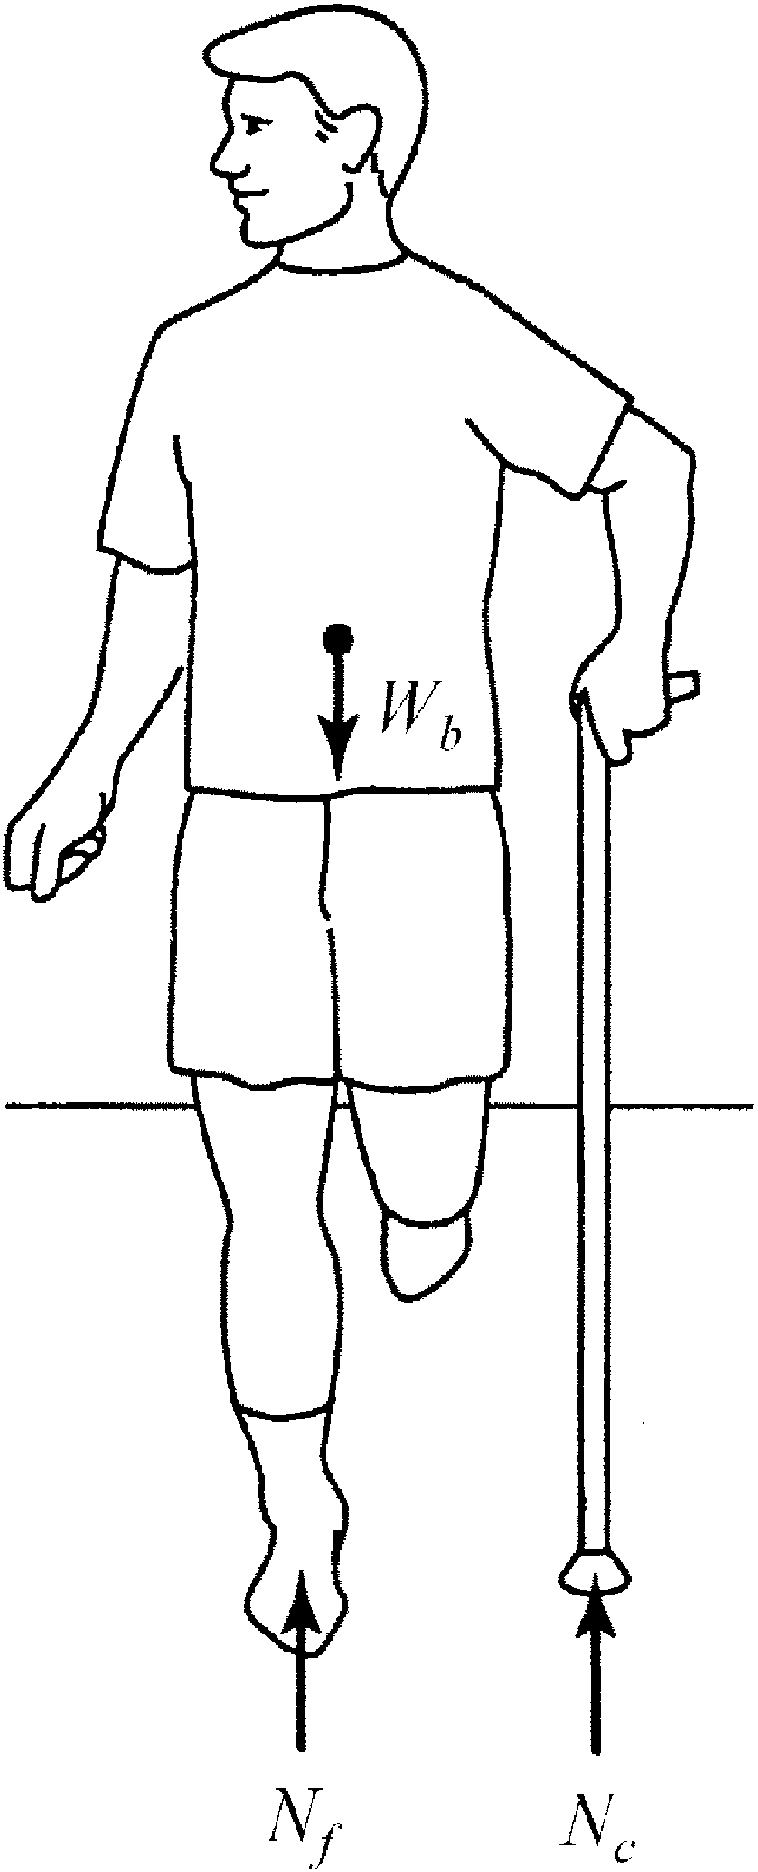
\includegraphics[width=0.5\textwidth]{218.png}
  \caption{Fuerzas sobre una persona completa para alguien caminando con un bastón. (De \cite{3}).}
  \label{fig:218}
\end{SCfigure}

\begin{SCfigure}[0.5][htbp]

  \centering
  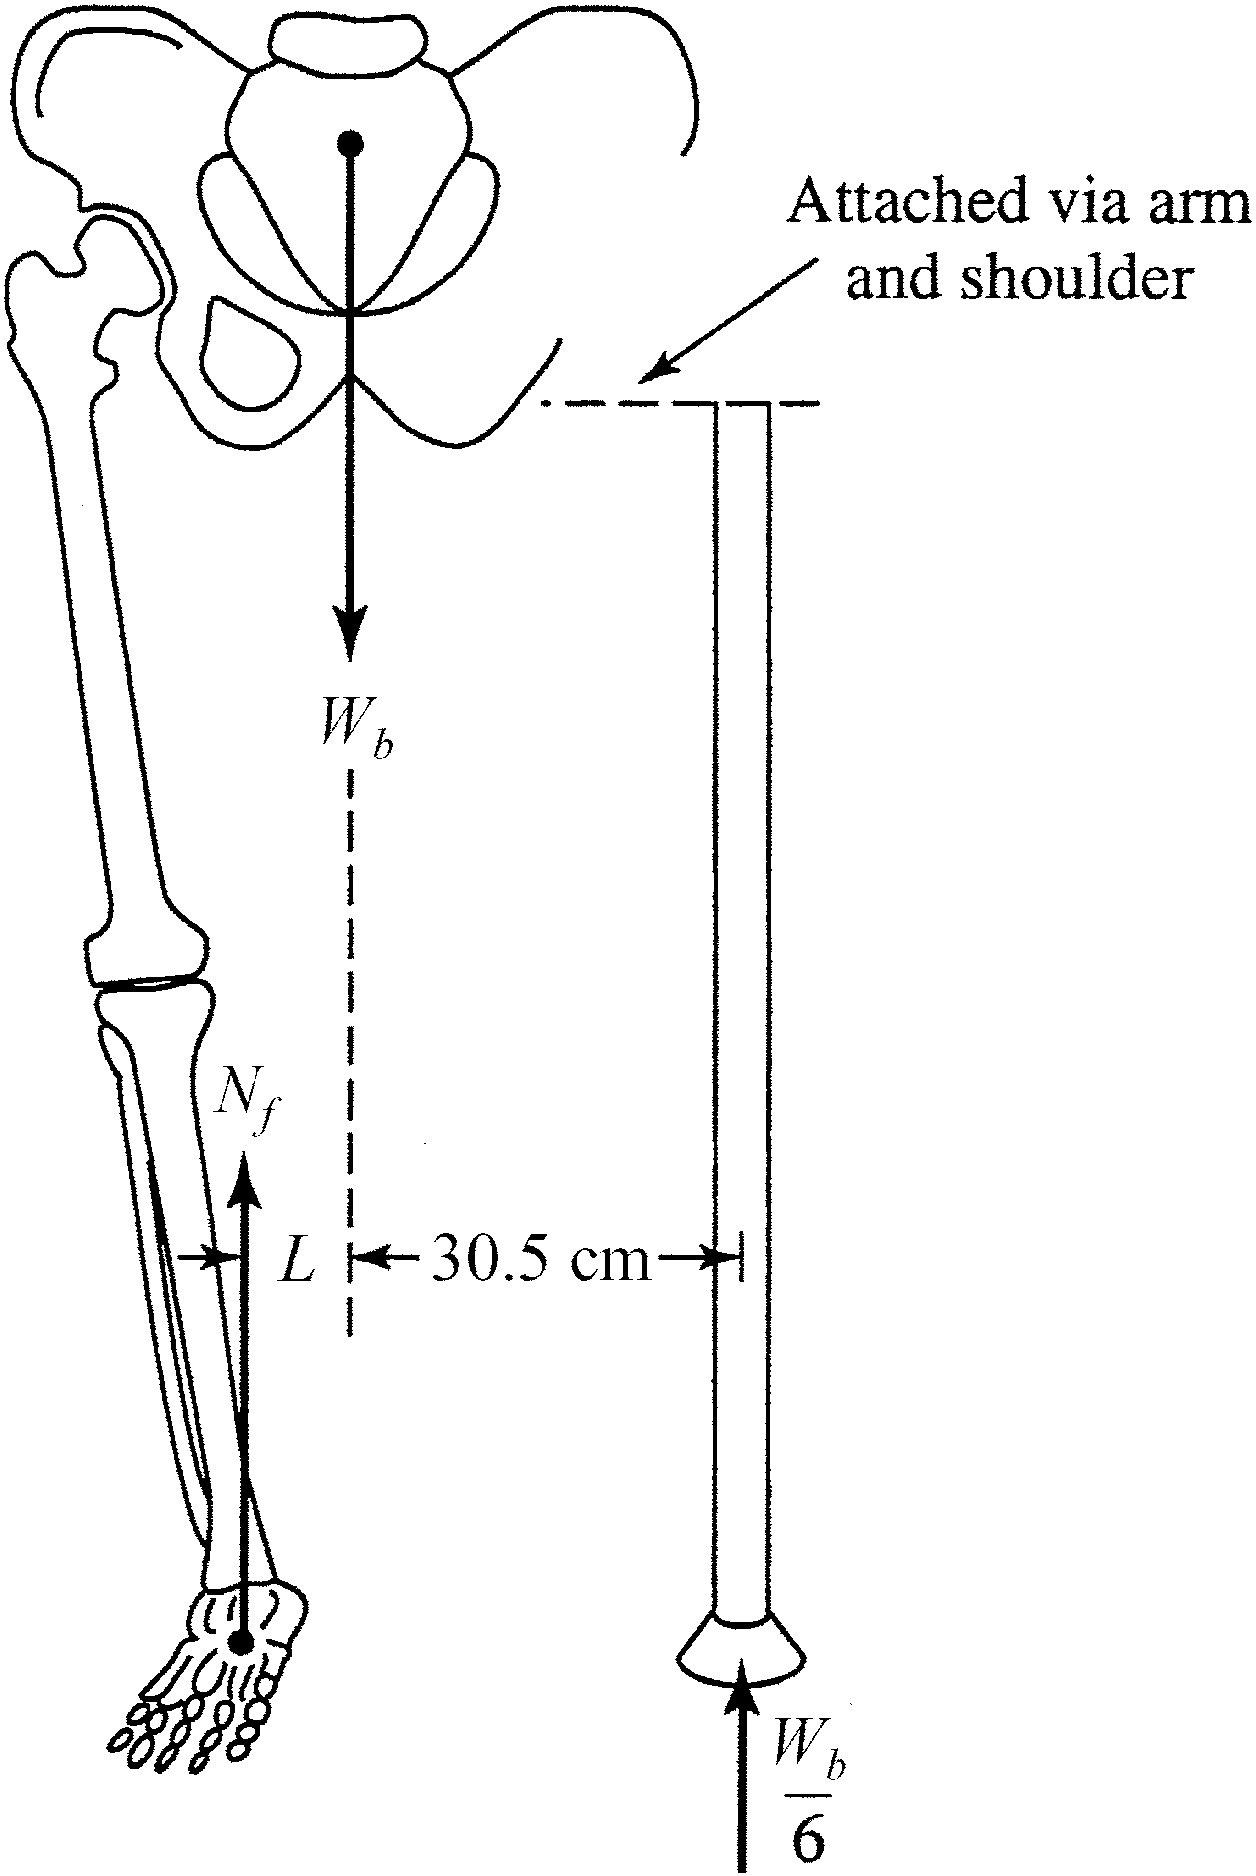
\includegraphics[width=0.5\textwidth]{219.png}
  \caption{Diagrama de fuerzas para una persona que usa un bastón como apoyo. (De \cite{3}).}
  \label{fig:219}
\end{SCfigure}

\begin{SCfigure}[0.5][htbp]

  \centering
  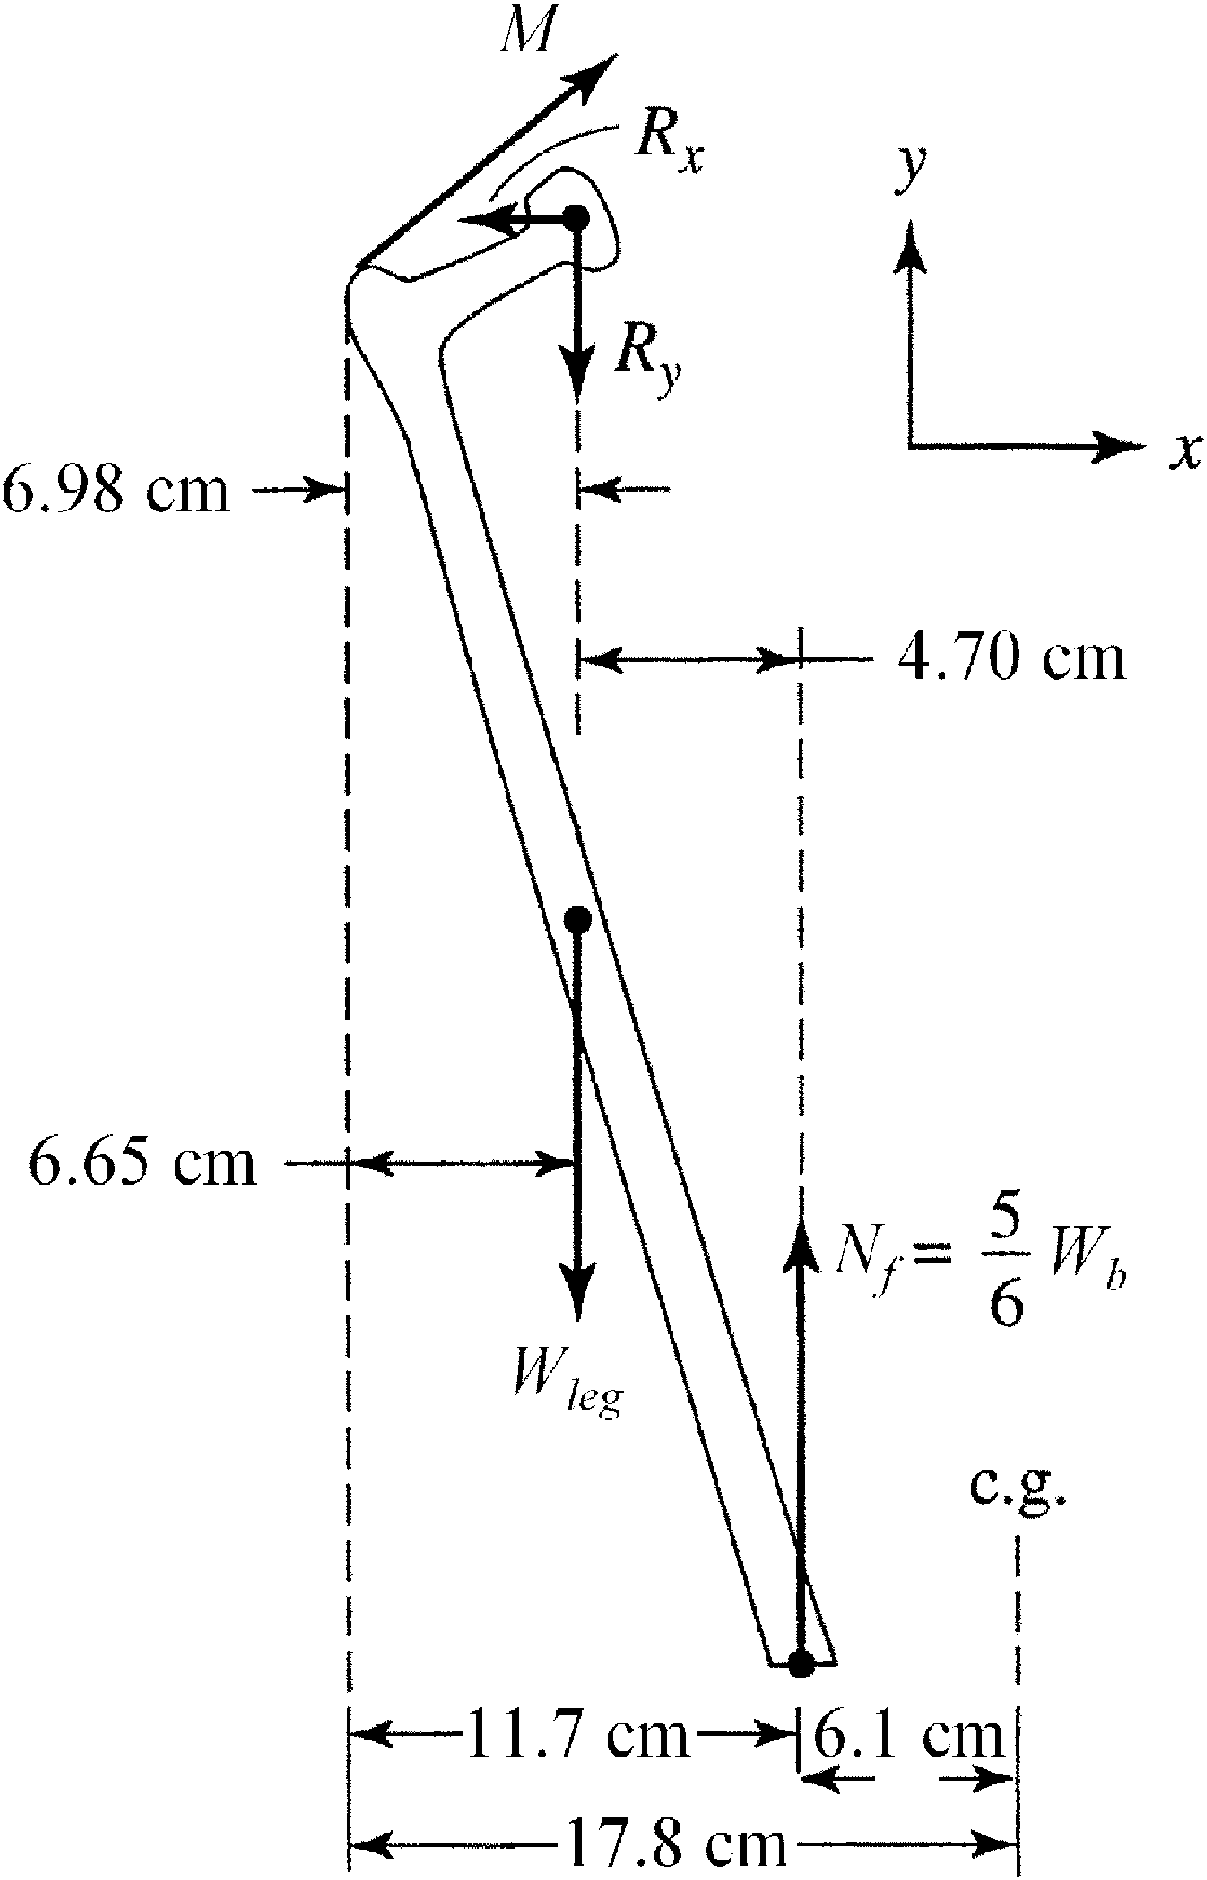
\includegraphics[width=0.5\textwidth]{220.png}
  \caption{Diagrama de fuerzas de cuerpo libre de la pierna para alguien caminando con un bastón. Observe que el centro de masa de la pierna está ahora a 0,33 cm a la izquierda de la vertical desde el centro de la cabeza del fémur, mientras que sin el bastón estaba a 3,2 cm a la derecha de la vertical. Por consiguiente, el centro de masa de la pierna está a 6,65 cm de la línea vertical desde el trocánter mayor, mientras que el centro de la cabeza del fémur está a 6,98 cm de ella. (De \cite{3}).}
  \label{fig:220}
\end{SCfigure}


\begin{equation}
F_x = M \cos 70^\circ - R_x = 0,
\label{eq:2.31}
\end{equation}
\begin{equation}
F_y = M \sin 70^\circ - R_y - 0,16 W_b + \frac{5}{6}W_b = 0,
\label{eq:2.32}
\end{equation}
\begin{equation}
\tau_z = +(4,7\text{ cm})\left(\frac{5}{6}\right)W_b + (0,33\text{ cm})(0,16 W_b) + 0 - (6,98\text{ cm})M \sin 70^\circ = 0.
\label{eq:2.33}
\end{equation}

La primera ecuación no ha cambiado. (Estamos asumiendo que el ángulo efectivo de los músculos abductores de la cadera con el eje $x$ sigue siendo $70^\circ$, aunque esto ya no sea rigurosamente cierto). El único cambio en la segunda ecuación es la fuerza normal menor sobre la pierna. Hay dos cambios en la ecuación de torque. El primer término, debido a la fuerza normal desde el suelo, es mucho menor debido al cambio en el brazo de momento y la fuerza normal de la pierna (siendo el primer efecto mucho mayor que el segundo). El segundo término, debido al peso de la pierna, es mucho menor en magnitud y ahora es un torque positivo en lugar de un torque negativo, porque el centro de masa de la pierna está ahora a la izquierda de la vertical trazada hacia abajo desde el eje (Figs. 2.2 y 2.20). Ahora $M = 0,61 W_b$, $R_x = 0,21 W_b$ y $R_y = 1,24 W_b$, con $R = 1,26 W_b$ y $\phi = 9,5^\circ$. Con $W_b$ aún en $880\text{ N}$ (200 lb), la fuerza muscular $M$ es ahora de $540\text{ N}$ (120 lb) (en lugar de $1400\text{ N}$ (320 lb) sin el bastón) y la fuerza de reacción en la cadera $R$ es ahora de $1100\text{ N}$ (250 lb) (en lugar de $2100\text{ N}$ (470 lb)). Este es un efecto muy grande, considerando que solo unos $145\text{ N}$ (35 lb) ($\approx W_b/6$) se apoyan en el bastón. Con diferencia, la consecuencia principal del bastón es el cambio del brazo de momento de la fuerza normal desde el suelo de $10,8$ a $4,7\text{ cm}$, debido a que el pie se desplazó hacia la derecha por $6,1\text{ cm}$.

Otra variación de esta situación se presenta en los Problemas 2.8 y 2.9. En lugar de usar un bastón con la mano izquierda, examinará las consecuencias de cargar un peso en el lado izquierdo. Esto aumenta enormemente los brazos de momento, incrementando por lo tanto $M$ y $R$. La Tabla 2.2 muestra estimaciones para las fuerzas máximas de la cadera para varias actividades a partir de análisis más detallados.

\begin{table}[htbp]
\centering
\caption{Estimaciones analíticas de las fuerzas máximas en la cadera para diversas actividades.}
\label{tab:22}
\begin{tabularx}{0.8\textwidth}{l>{\centering\arraybackslash}X}
\toprule
\textbf{Actividad} & \textbf{Magnitud/peso corporal, $W_b$} \\
\midrule
Caminar & 4,8--5,5 \\
Caminar lentamente con/sin bastón & 2,2/3,4 \\
Subir escaleras & 7,2--7,4 \\
Bajar escaleras & 7,1 \\
Levantarse de una silla & 3,3 \\
\bottomrule
\end{tabularx}
\begin{flushleft}
    \small Utilizando datos de \cite{24}
\end{flushleft}
\end{table}

Las fuerzas excesivas en la cadera durante períodos prolongados de tiempo pueden desgastar el cartílago y causar otros daños; esto provoca dolor al caminar que a veces solo puede aliviarse con un reemplazo de cadera. Los reemplazos totales de cadera implican reemplazar la bola del fémur y el acetábulo. El componente femoral es una bola altamente pulida de una aleación de alta resistencia, como cobalto-cromo o titanio, con un vástago que se coloca en el canal del fémur. A menudo se fija con un plástico acrílico, como el poli(metacrilato de metilo), PMMA (por sus siglas en inglés, \textit{poly(methyl methacrylate)}), «cemento óseo». El componente del acetábulo es una cavidad hecha de polietileno de peso molecular ultra alto y puede tener un refuerzo metálico.

\subsection{Estática de otras articulaciones sinoviales}

Otras articulaciones sinoviales se pueden examinar de manera similar utilizando modelos de los músculos y tendones. Se describen brevemente aquí; ver \cite{28} para más detalles.

\textbf{Hombro}\\
La anatomía y la musculatura del hombro se muestran en las Figs. 1.2 y 1.8. La Figura 2.21 muestra un modelo del equilibrio estático de un brazo horizontal que sostiene un peso por medio del músculo deltoides. Este peso y el músculo están en equilibrio con el peso del brazo y la fuerza de reacción en la articulación. Los Problemas 2.16 a 2.18 abordan esto con y sin un peso sostenido en la mano. Para parámetros razonables, la componente de la fuerza muscular en la dirección $x$ es aproximadamente 4 veces la de la dirección $y$, lo que sugiere que sostener el brazo horizontalmente no es estable, como todos sabemos.

\begin{SCfigure}[0.5][htbp]

  \centering
  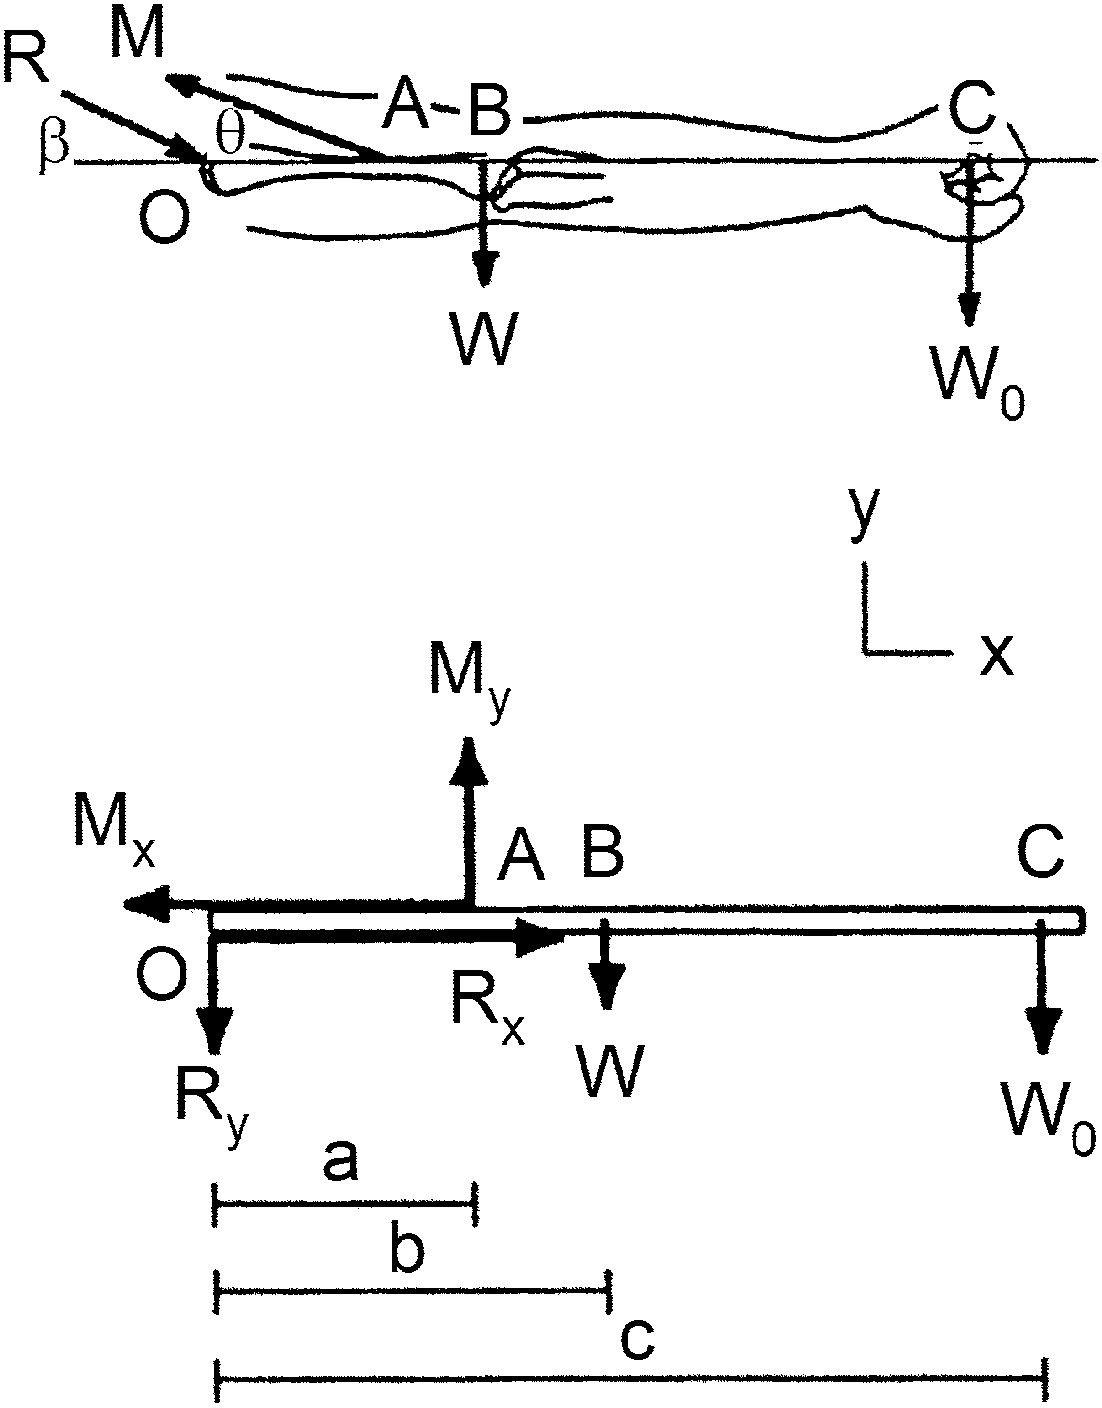
\includegraphics[width=0.5\textwidth]{221.png}
  \caption{Fuerzas sobre el brazo y el hombro, cuando el brazo está abducido a la posición horizontal y la mano sostiene un peso, junto con el diagrama de fuerzas. (De \cite{28}).}
  \label{fig:221}
\end{SCfigure}



La dislocación de la articulación del hombro (glenohumeral) es común porque es poco profunda. El gran grado de movimiento rotacional de la cabeza del húmero alrededor de la superficie de articulación de la cavidad glenoidea permite este gran movimiento, aunque con poca estabilidad. Los ángulos de la articulación del hombro varían en $\sim 249^\circ$ durante la flexión/extensión, $\sim 182^\circ$ en la abducción/aducción y $\sim 131^\circ$ para la rotación interna/externa (Tabla 1.10). La fractura del húmero también es relativamente común.

\textbf{Rodilla}\\
La articulación de la rodilla es en realidad dos articulaciones (Fig. 1.3). La articulación tibiofemoral se encuentra entre los cóndilos medial y lateral del fémur y la tibia, los cuales están separados por regiones cartilaginosas llamadas meniscos. (Un cóndilo es la prominencia redondeada al final de un hueso, a menudo en una articulación). La segunda es la articulación patelofemoral entre la rótula (\textit{patella}) y el extremo anterior de los cóndilos femorales. El control muscular de la rodilla se realiza principalmente a través de los músculos cuádriceps e isquiotibiales (\textit{hamstring}). Los cuádriceps se unen al tendón del cuádriceps, el cual se une a la rótula, la cual se une al tendón patelar, el cual se une a la tibia. La Figura 2.22 muestra algunos de los músculos principales de la pierna.

\begin{figure}[htbp]

  \centering
  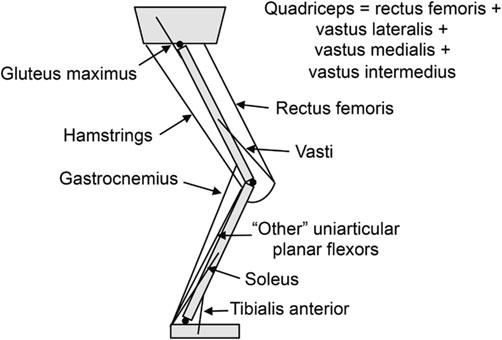
\includegraphics[width=0.75\textwidth]{222.png}
  \caption{Músculos principales de la pierna. (Basado en \cite{9}).}
  \label{fig:222}
\end{figure}



Las fuerzas sobre la pantorrilla estática cargada con una pesa en el tobillo, como durante el ejercicio (Fig. 2.23), se muestran en las Figs. 2.24 y 2.25. Las fuerzas mostradas se deben a este peso añadido, al peso de la pantorrilla, a la fuerza del músculo cuádriceps transmitida por el tendón patelar $\vec{\mathbf{M}}$ (de magnitud $M$) y a la fuerza de reacción de la articulación $\vec{\mathbf{R}}$ (de magnitud $R$), mientras que el ángulo entre la horizontal y la pierna es $\beta$. En equilibrio, la fuerza muscular y las componentes $x$ e $y$ de la fuerza de la articulación son

\begin{figure}[htbp]

  \centering
  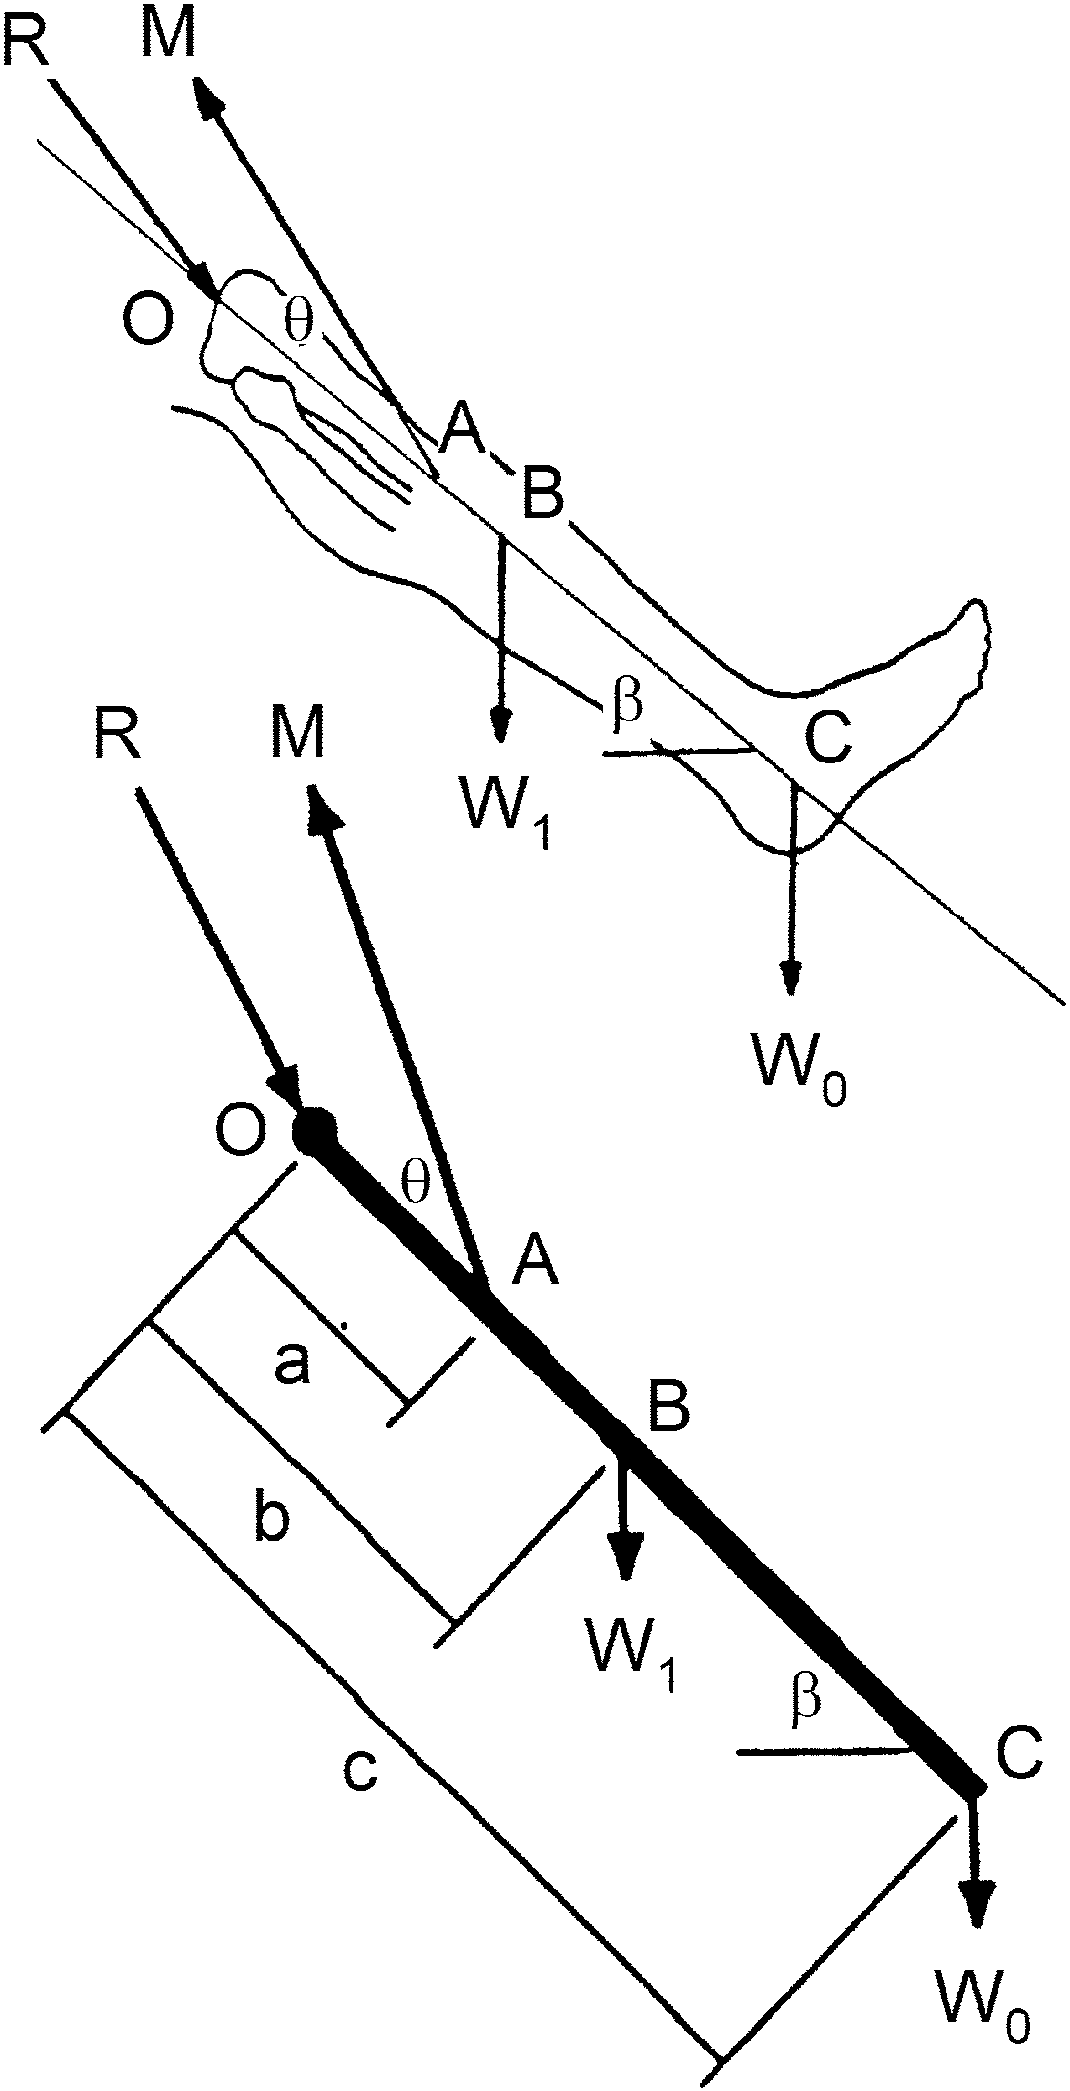
\includegraphics[width=0.55\textwidth]{223.png}
  \caption{Ejercicio de los músculos cerca y en la rodilla. (De \cite{28}).}
  \label{fig:223}
\end{figure}

\begin{SCfigure}[0.5][htbp]

  \centering
  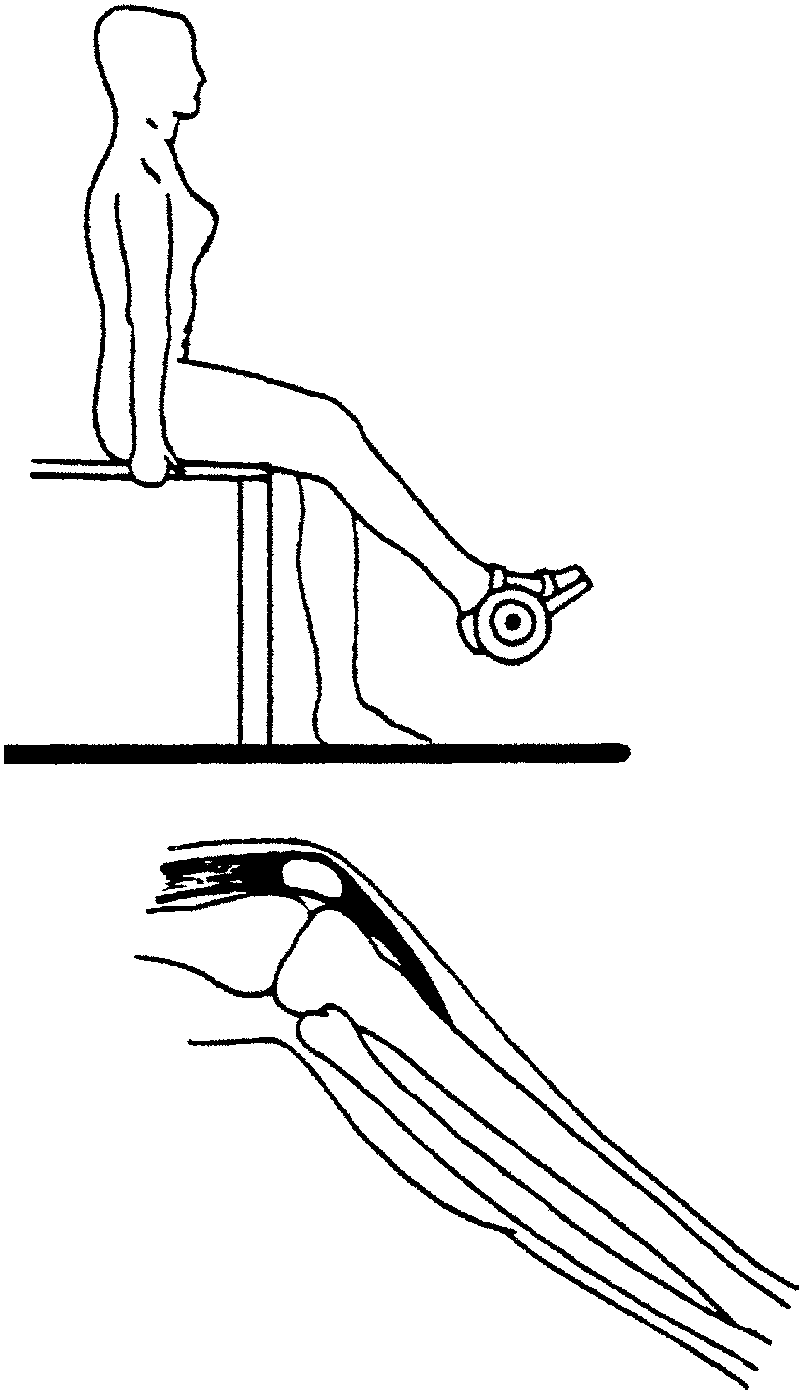
\includegraphics[width=0.5\textwidth]{224.png}
  \caption{Fuerzas sobre la pantorrilla (pierna inferior), durante el ejercicio del músculo al rededor de la rodilla. (De \cite{28}).}
  \label{fig:224}
\end{SCfigure}

\begin{SCfigure}[0.5][htbp]

  \centering
  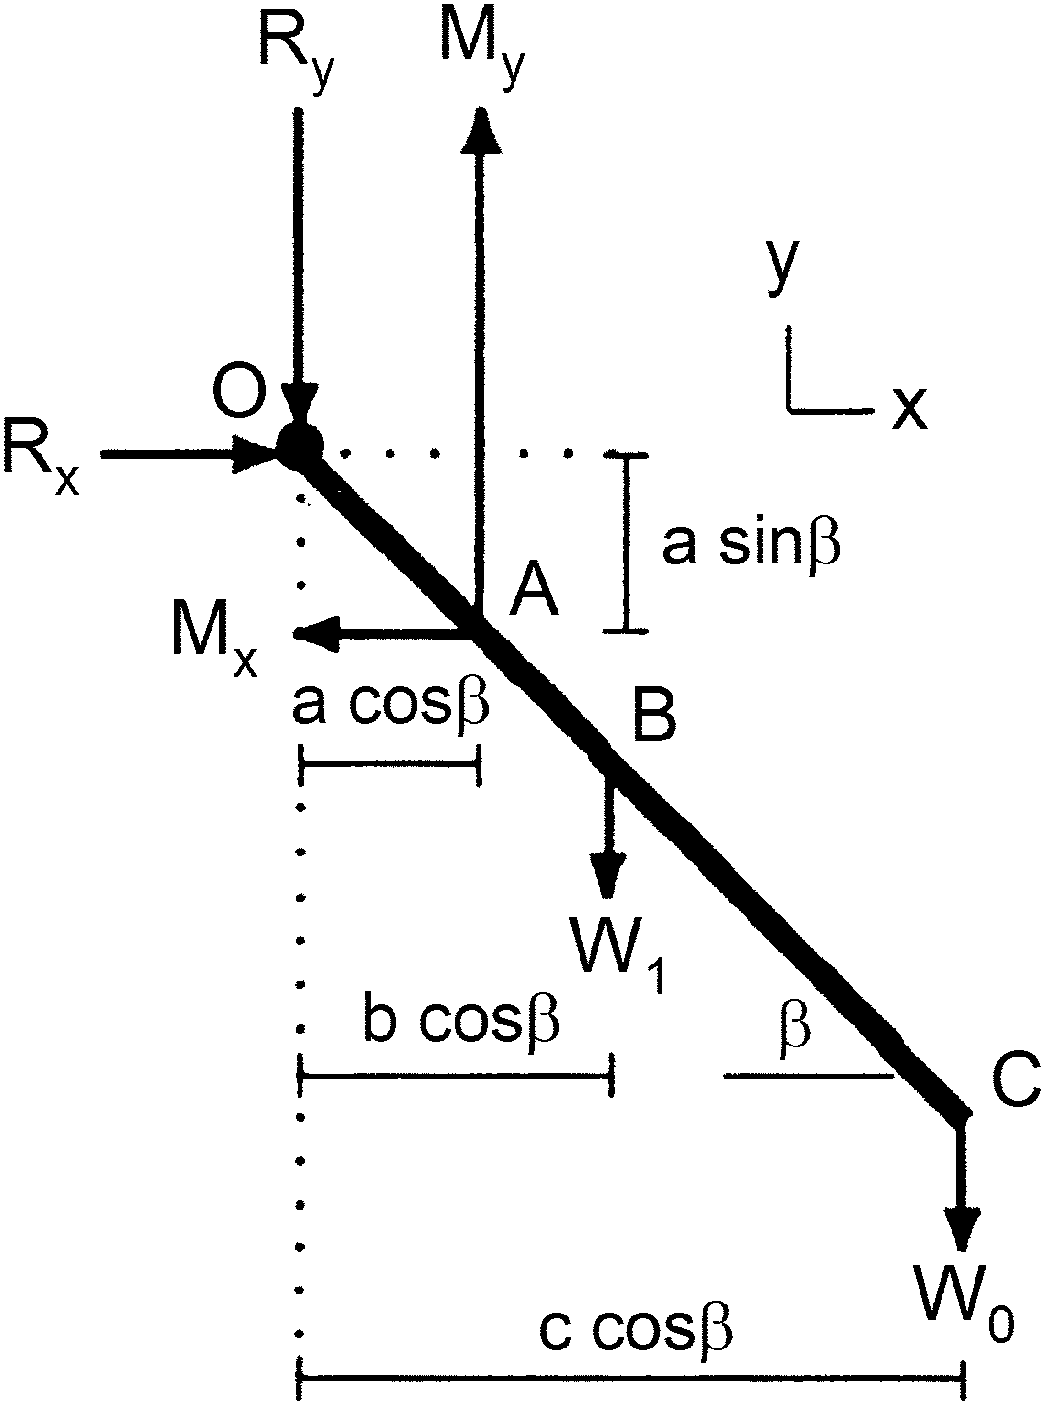
\includegraphics[width=0.5\textwidth]{225.png}
  \caption{Descomposición de las fuerzas sobre la pantorrilla en la Fig. 2.24. (De \cite{28}).}
  \label{fig:225}
\end{SCfigure}


\begin{equation}
M = \frac{(b W_1 + c W_0) \cos \beta}{a \sin \theta},
\label{eq:2.34}
\end{equation}
\begin{equation}
R_x = M \cos(\theta + \beta),
\label{eq:2.35}
\end{equation}
\begin{equation}
R_y = M \sin(\theta + \beta) - W_0 - W_1.
\label{eq:2.36}
\end{equation}

Estas fuerzas son muy grandes \cite{26, 28}. Para $a = 12\text{ cm}$, $b = 22\text{ cm}$, $c = 50\text{ cm}$, $W_1 = 150\text{ N}$, $W_0 = 100\text{ N}$, $\theta = 15^\circ$ y $\beta = 45^\circ$, vemos que la fuerza muscular $M = 1381\text{ N}$ y la fuerza de la articulación $R = 1171\text{ N}$. Esto se examina con más detalle en el Problema 2.19. Los Problemas 2.22 a 2.25 abordan una condición relacionada, la de la posición en cuclillas, como ocurre al subir y bajar escaleras o al saltar.

Una función de la rótula es servir como una polea mecánica para aumentar el torque incrementando el brazo de momento (Fig. 2.26). Podemos analizar el equilibrio de la rótula en la articulación patelofemoral entre la fuerza de reacción sobre la rótula desde el extremo anterior de los cóndilos femorales, el tendón patelar y el tendón del cuádriceps. Esto se muestra en la Fig. 2.27. La fuerza de compresión aplicada sobre la rótula es

\begin{SCfigure}[0.5][htbp]

  \centering
  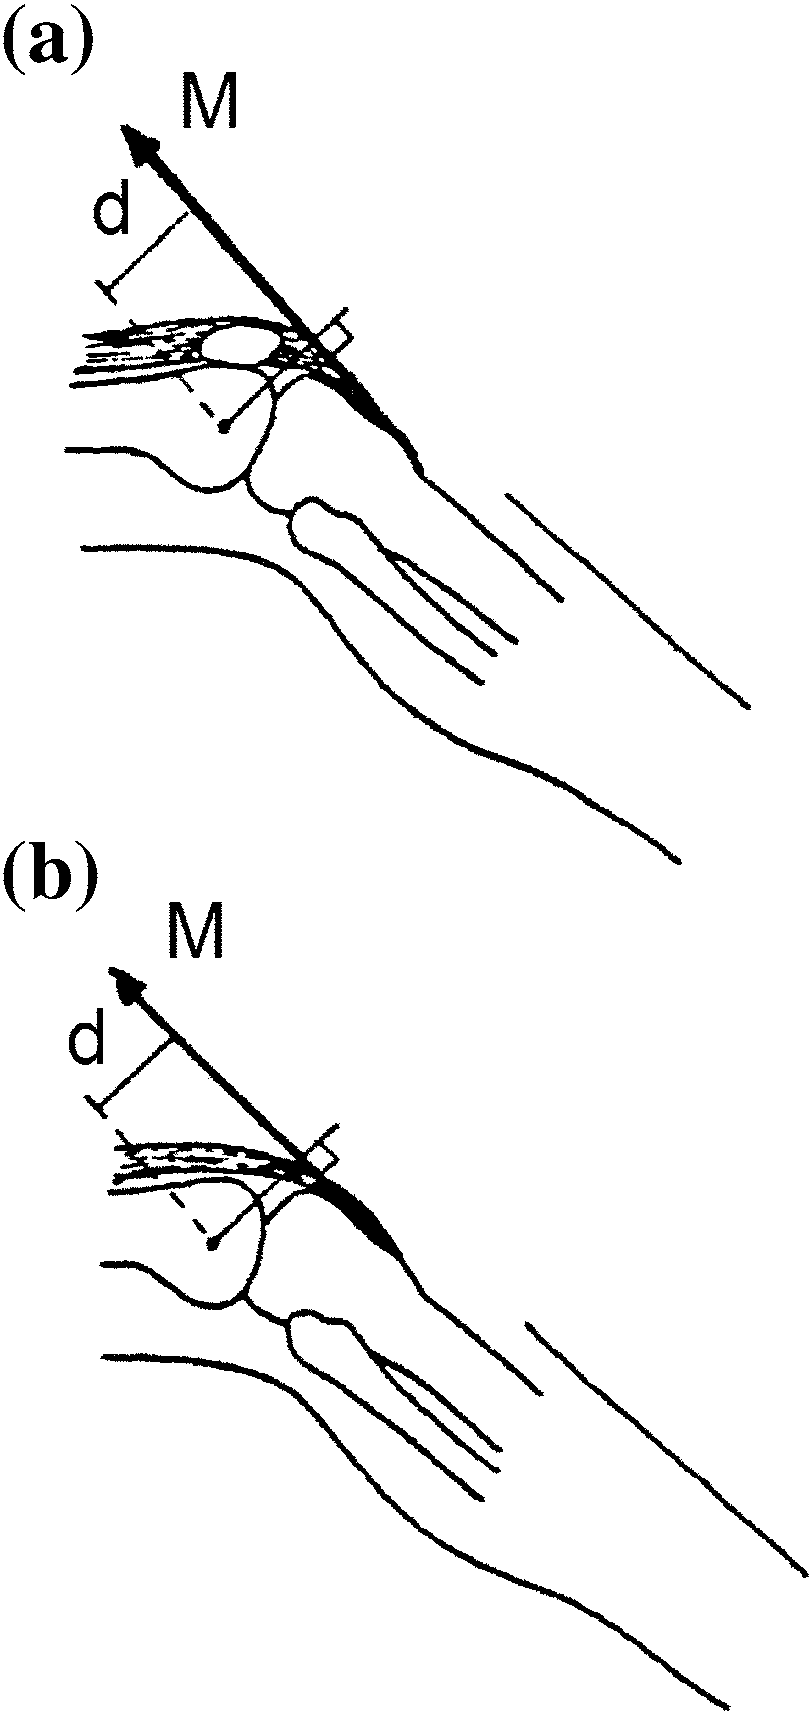
\includegraphics[width=0.5\textwidth]{226.png}
  \caption{La presencia de la rótula (patela) aumenta el brazo de momento en la palanca. (De \cite{28}).}
  \label{fig:226}
\end{SCfigure}

\begin{SCfigure}[0.5][htbp]

  \centering
  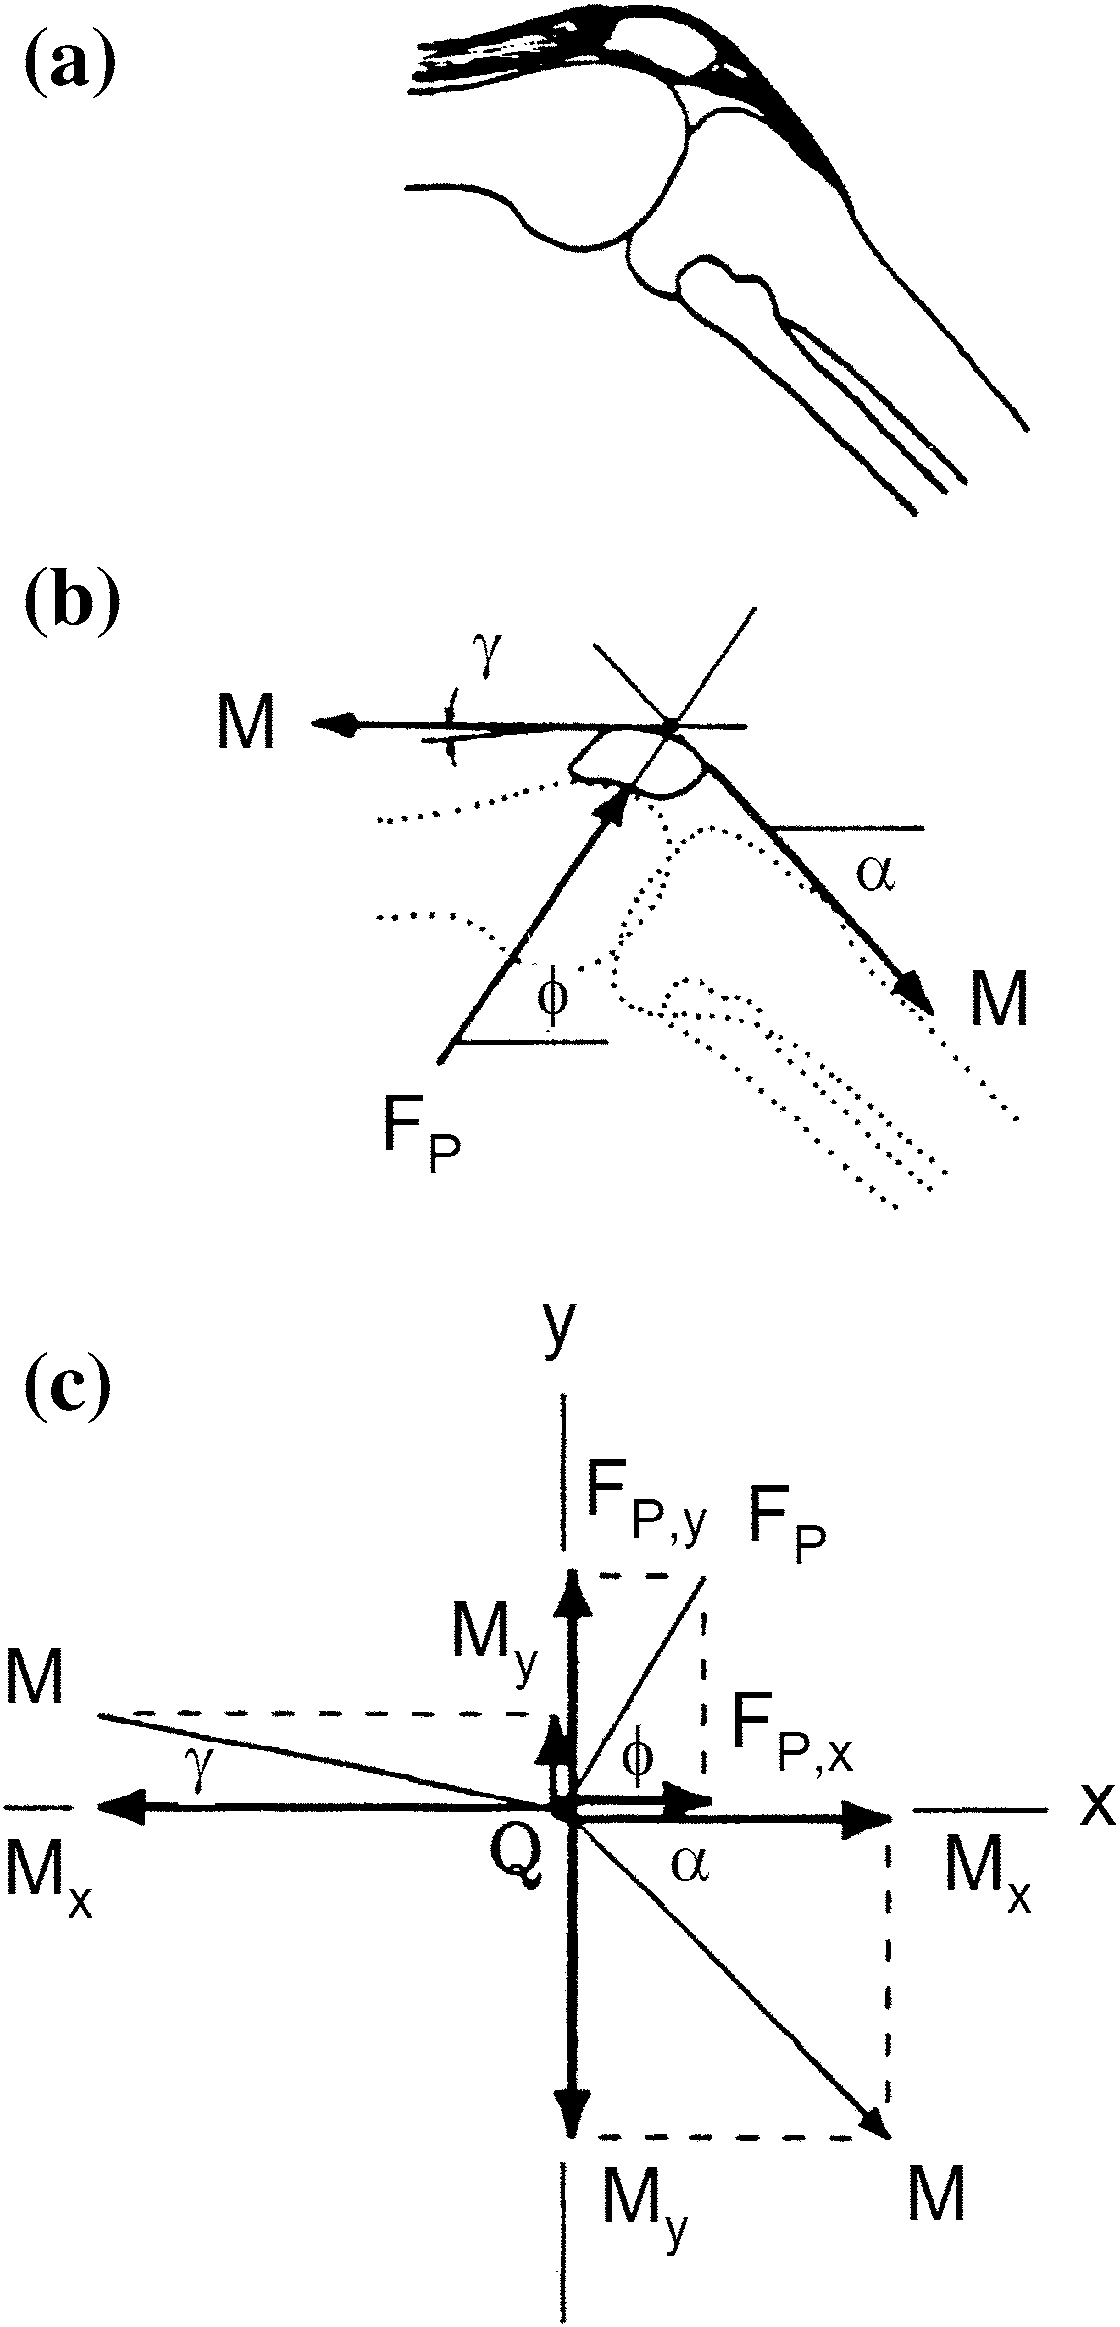
\includegraphics[width=0.5\textwidth]{227.png}
  \caption{Diagrama de fuerzas de la rótula (patela) en equilibrio. (De \cite{28}).}
  \label{fig:227}
\end{SCfigure}


\begin{equation}
F_P = \frac{\cos \gamma - \cos \alpha}{\cos \phi} M
\label{eq:2.37}
\end{equation}
a un ángulo
\begin{equation}
\phi = \arctan \left( \frac{\sin \alpha - \sin \gamma}{\cos \gamma - \cos \alpha} \right).
\label{eq:2.38}
\end{equation}

\textbf{Tobillo}\\
Ahora examinamos el equilibrio del pie. La anatomía del tobillo y del pie se representa en las Figs. 2.14 y 2.15 (ver también las Figs. 1.8 y 3.5). Las Figuras 2.28 y 2.29 muestran las fuerzas cuando alguien se para de puntillas sobre un pie. La fuerza de reacción sobre el hueso astrágalo (\textit{talus}) del pie está en equilibrio con la fuerza normal desde el suelo (igual al peso corporal) y la fuerza muscular transmitida por el tendón de Aquiles sobre el calcáneo (talón). (La masa del pie en sí se desprecia aquí). Las fuerzas muscular y de reacción son
\begin{equation}
M = W_b \frac{\cos \beta}{\cos(\theta + \beta)},
\label{eq:2.39}
\end{equation}
\begin{equation}
R = W_b \frac{\cos \theta}{\cos(\theta + \beta)}.
\label{eq:2.40}
\end{equation}

Ambas son mucho mayores que el peso corporal $W_b$. Para $\theta = 45^\circ$ y $\beta = 60^\circ$, vemos que $M = 1,93 W_b$ y $R = 2,73 W_b$.

\begin{SCfigure}[0.5][htbp]

  \centering
  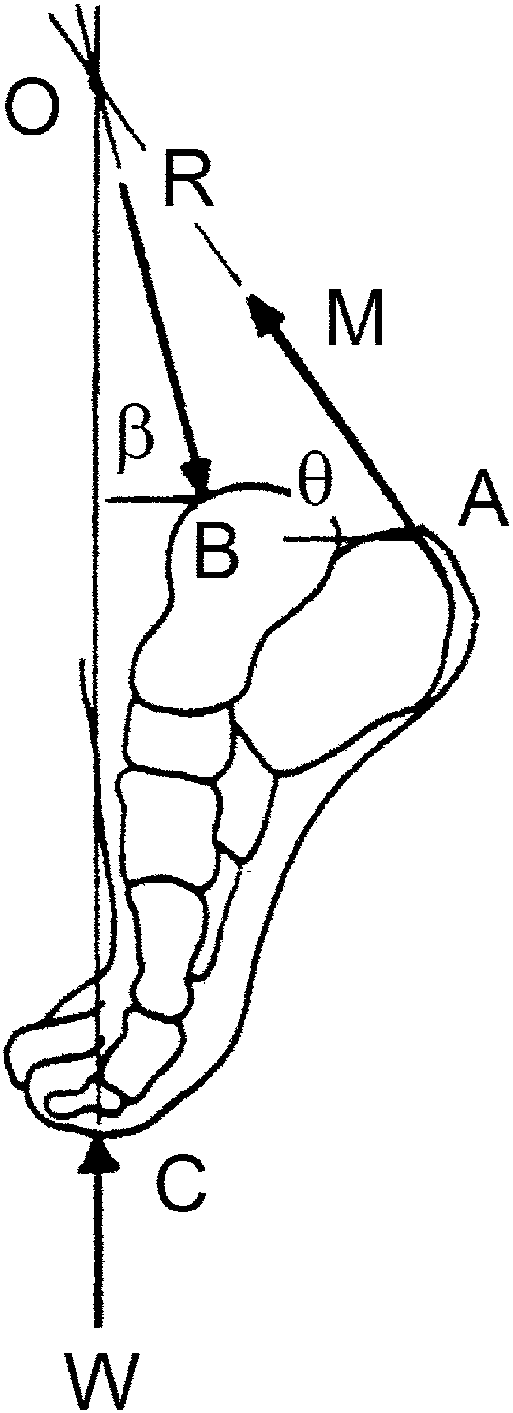
\includegraphics[width=0.5\textwidth]{228.png}
  \caption{Diagrama de fuerzas del pie de puntillas, mostrando que forman un sistema concurrente. (De \cite{28}).}
  \label{fig:228}
\end{SCfigure}

\begin{SCfigure}[0.5][htbp]

  \centering
  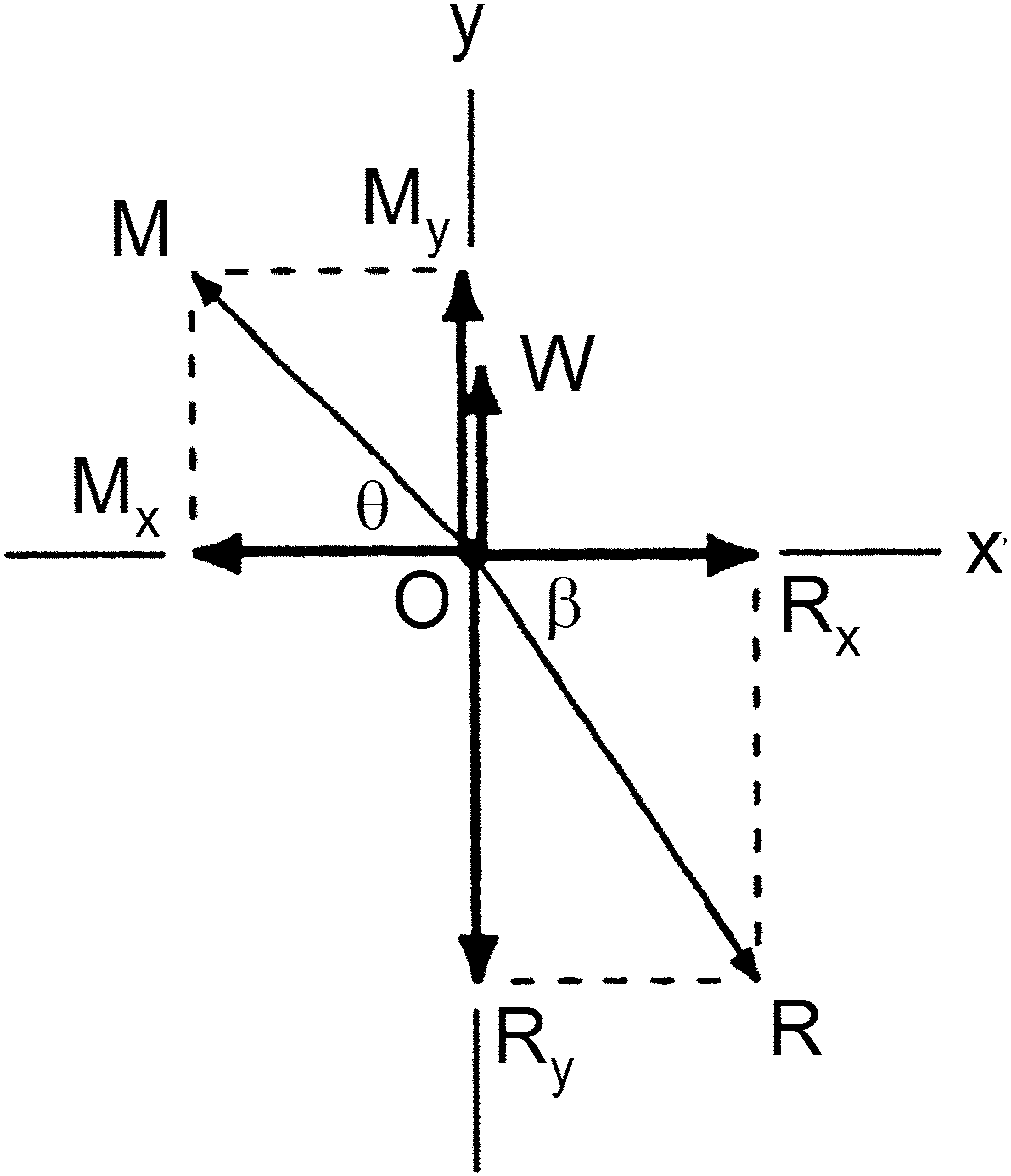
\includegraphics[width=0.5\textwidth]{229.png}
  \caption{Componentes de las fuerzas que actúan sobre un pie de puntillas. (De \cite{28}).}
  \label{fig:229}
\end{SCfigure}



\subsubsection{Mandíbulas y dientes}

Si nuestras mandíbulas consistieran en dos huesos, cada uno con dientes de igual tamaño sobre un plano que emana de las articulaciones articulares, todos o muchos de nuestros dientes no podrían tocarse entre sí durante la masticación; los dientes posteriores se tocarían primero y entonces los dientes anteriores no podrían tocarse. Afortunadamente, esto no ocurre porque hay un ángulo recto en nuestra mandíbula, el hueso de la mandíbula inferior. Las partes de la rama (\textit{ramus}), a cada lado de la mandíbula (Fig. 2.30), se conectan a los dos huesos temporales a través de las articulaciones de bisagra articular temporomandibular a cada lado de la mandíbula. Cada rama está unida al cuerpo de la mandíbula, que contiene los dientes de la mandíbula inferior, de manera perpendicular, de modo que muchos de nuestros dientes pueden tocarse entre sí al mismo tiempo \cite{16}. (El maxilar sostiene los dientes superiores).

Lateralmente desde la línea media en cualquiera de las mandíbulas, tenemos ocho dientes: dos incisivos, un canino (o colmillo), dos bicúspides (o premolares) y tres molares (siendo el último molar la muela del juicio). (Este orden de los dientes se puede recordar por su acrónimo: ICBM ---el cual en sí es fácil de recordar porque también es el acrónimo de los Misiles Balísticos Intercontinentales [\textit{Intercontinental Ballistic Missiles}]---). Las protuberancias de los dientes se denominan cúspides, teniendo los caninos una, los bicúspides dos y los molares cuatro o cinco. Las fuerzas sobre los dientes surgen de varias fuentes \cite{12}. La Figura 2.30 muestra cómo los músculos maseteros proporcionan la fuerza en el sistema de palanca involucrado en la masticación y la mordida. Se pueden utilizar modelos de palanca para examinar la cuasiestática de la masticación y la mordida. En la mandíbula, las ventajas mecánicas de los músculos maseteros son 0,50 y 0,76 para el incisivo y el primer molar (anterior), y de manera similar para los músculos temporal anterior y temporal posterior son 0,24 y 0,48, y 0,37 y 0,72, respectivamente (para hombres y ligeramente menores para mujeres) (ver Problema 2.28) \cite{34}. Estas fuerzas durante la masticación deben entenderse en el contexto de las propiedades mecánicas de los alimentos, que se analizan en el Cap. 4; la masticación claramente afecta cómo digerimos los alimentos (ver Cap. 6).

La ortodoncia es la aplicación práctica de la biomecánica para mover los dientes utilizando fuerzas aplicadas por aparatos, tales como alambres, brackets y elásticos \cite{23, 29, 32}. Cada diente tiene un centro de masa, pero dado que los dientes no son cuerpos libres ---están limitados por el periodonto--- se define una posición más útil en el diente, el centro de resistencia. Este es el punto de equilibrio para el diente. La Figura 2.31 muestra cómo las fuerzas y los torques (momentos) aplicados a la corona de un diente pueden diseñarse para crear una fuerza lateral en el centro de resistencia, pero ningún torque alrededor del mismo. Los aparatos pueden afectar a varios dientes, como el arco de intrusión mostrado en la Fig. 2.32, lo que conduce a la aplicación de las fuerzas y torques que se muestran en la Fig. 2.33.

\begin{SCfigure}[0.5][htbp]

  \centering
  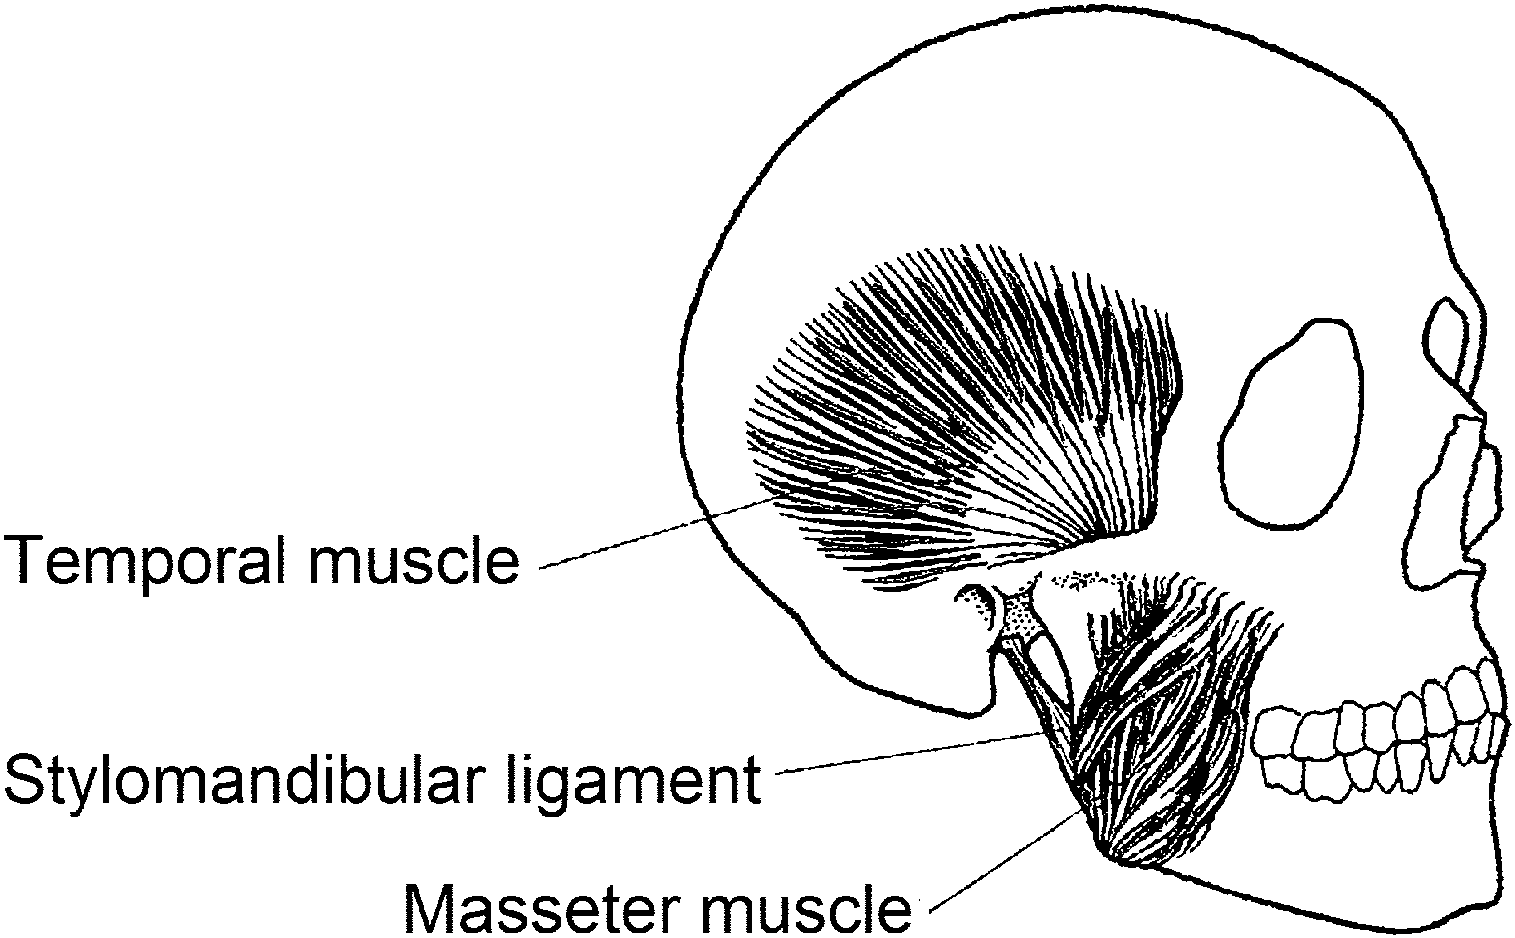
\includegraphics[width=0.55\textwidth]{230.png}
  \caption{Los músculos masetero y temporal en la mandíbula, alrededor de la articulación temporomandibular. La mandíbula es el hueso de la mandíbula inferior, y sus ramas son las que se muestran cubiertas por los músculos maseteros. (De \cite{30}).}
  \label{fig:230}
\end{SCfigure}

\begin{SCfigure}[0.5][htbp]

  \centering
  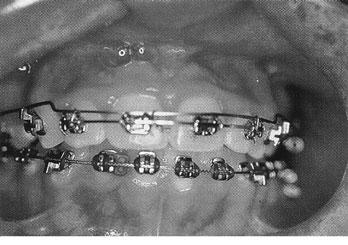
\includegraphics[width=0.55\textwidth]{231.png}
  \caption{En ortodoncia se aplican fuerzas y torques a la corona (izquierda), lo que conduce a fuerzas (y en este caso ningún torque) alrededor del centro de resistencia. (Reimpreso de \cite{23}. Usado con permiso de Elsevier).}
  \label{fig:231}
\end{SCfigure}

\begin{SCfigure}[0.5][htbp]

  \centering
  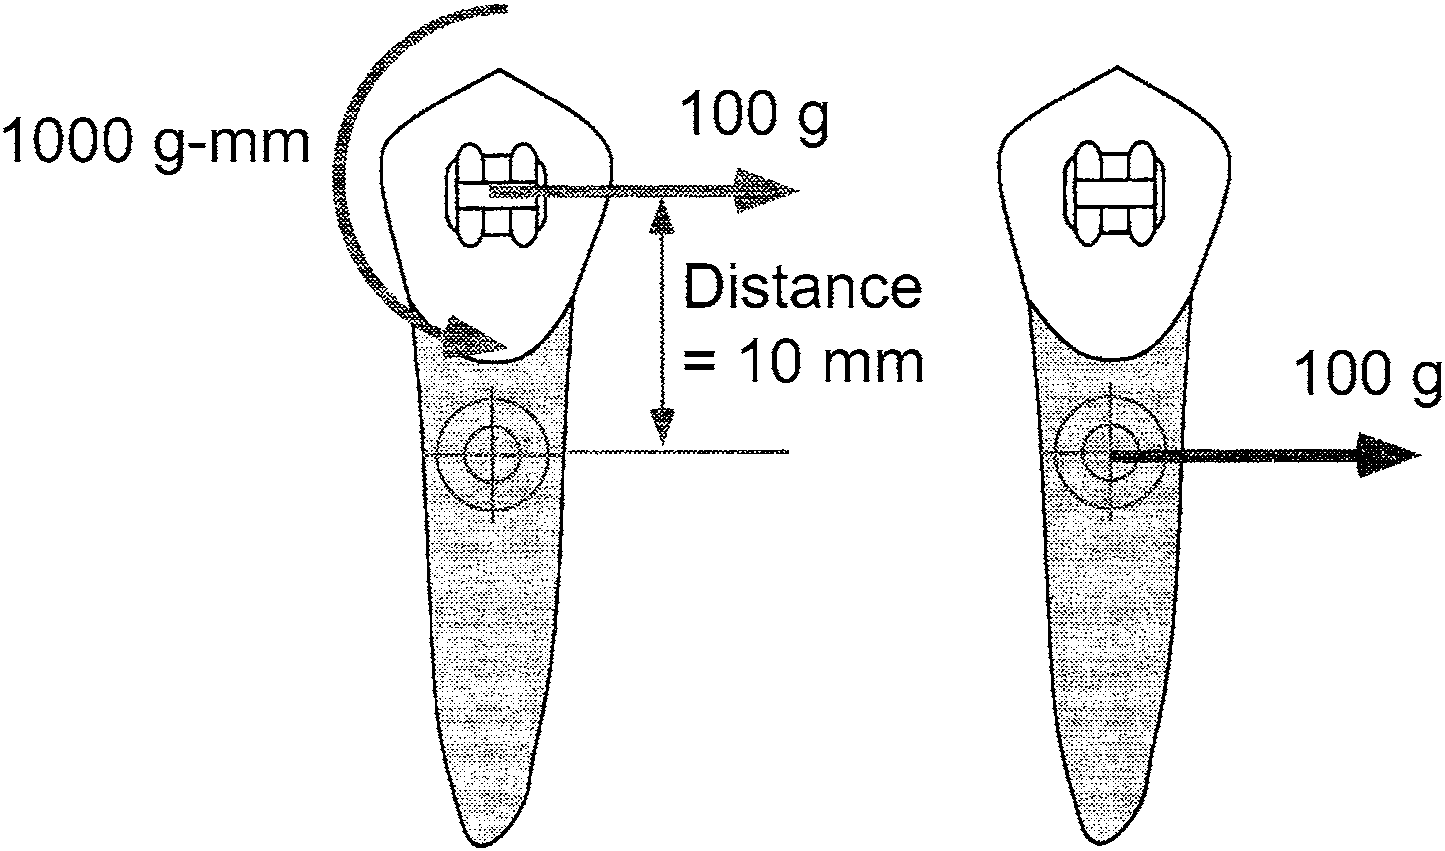
\includegraphics[width=0.55\textwidth]{232.png}
  \caption{Foto de un arco de intrusión utilizado en ortodoncia. (Reimpreso de \cite{23}. Usado con permiso de Elsevier).}
  \label{fig:232}
\end{SCfigure}

\begin{SCfigure}[0.5][htbp]

  \centering
  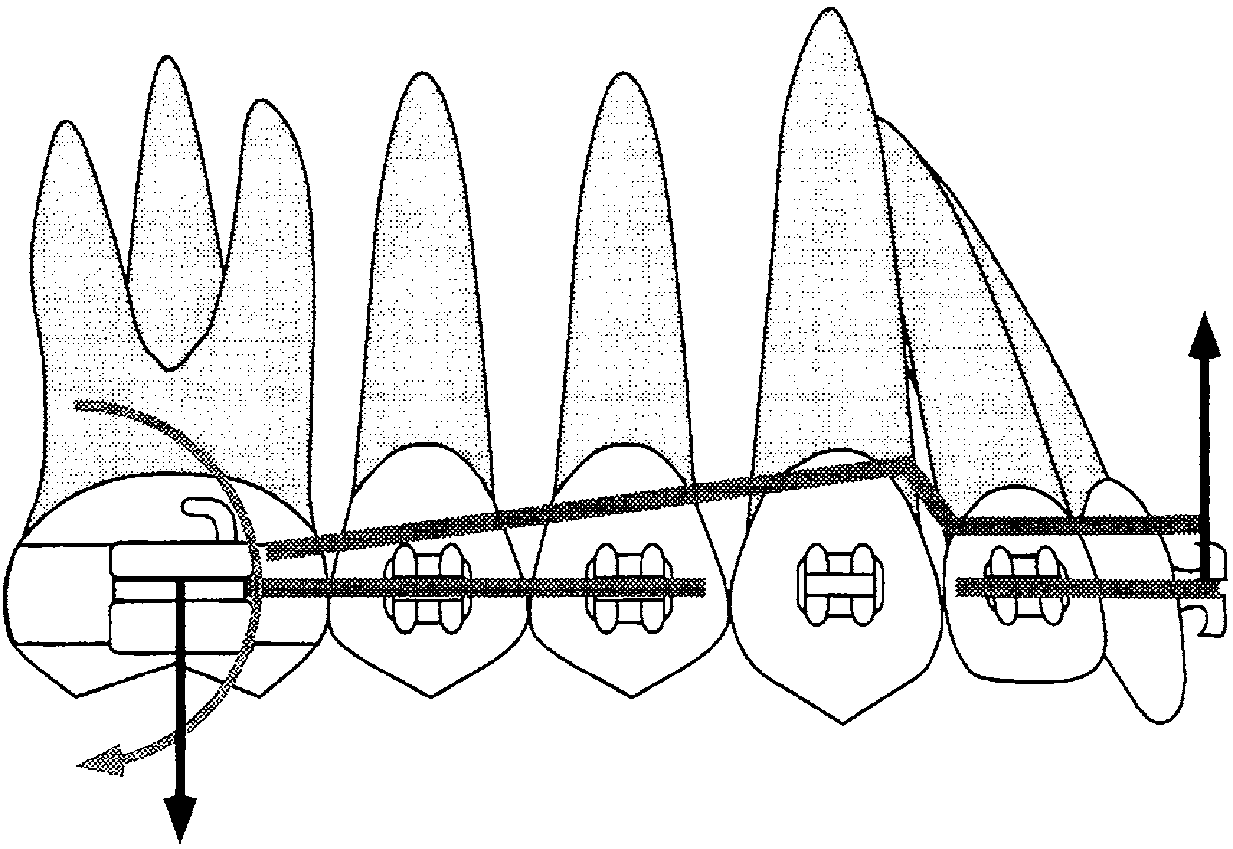
\includegraphics[width=0.55\textwidth]{233.png}
  \caption{Fuerzas y torques aplicados por el arco de intrusión en la Fig. 2.32. (Reimpreso de \cite{23}. Usado con permiso de Elsevier).}
  \label{fig:233}
\end{SCfigure}



¿Por qué tantos niños y adultos jóvenes necesitan ortodoncia para corregir la alineación de la mandíbula y los dientes en primer lugar? Además, ¿por qué a menudo necesitan que se les extraigan varios dientes, frecuentemente las muelas del juicio (los terceros molares)? Estos problemas sugieren que tienen demasiados dientes o mandíbulas demasiado pequeñas. Algunos piensan que los niños comen alimentos tan blandos que sus huesos maxilares en crecimiento no sienten las tensiones que normalmente ocurrirían al masticar alimentos más duros (como lo habrían hecho hace muchísimos años), y por lo tanto sus mandíbulas nunca crecen para ser tan anchas y fuertes como podrían serlo, para un conjunto de genes dado \cite{16, 17}. Si es así, las fuerzas aplicadas por la ortodoncia están sustituyendo a las perdidas por masticar alimentos blandos. (En el Cap. 4 se presenta un ejemplo claro de cómo las cargas afectan el crecimiento óseo, en relación con el crecimiento de los huesos largos).

\subsection{Problemas de la parte baja de la espalda}

La mayoría de las personas desarrollan eventualmente problemas crónicos en la parte baja de la espalda. La mejor manera de evitar un problema tan persistente y molesto es intentar evitar situaciones que puedan desencadenar su primer problema de espalda, como agacharse y levantar objetos pesados, o dormir en camas muy duras. Examinaremos un modelo estático simple que mostrará por qué nunca se debe doblar la espalda y levantar objetos. (Se deben usar los músculos de las piernas para levantar y no los de la espalda). Examinaremos la fuerza sobre la quinta vértebra lumbar cuando se dobla la espalda y se levanta un objeto.

La columna vertebral consta de 33 vértebras con 26 huesos y se clasifica en cinco secciones. Comenzando desde la parte superior (superior) en la Fig. 2.34, hay siete vértebras cervicales, doce torácicas ---que rima con «jurásicas»--- y cinco lumbares, y luego cinco vértebras fusionadas en el sacro (\textit{sacrum}, pronunciado «sae'-krum») y cuatro vértebras fusionadas en el coxis (\textit{coccyx}, pronunciado «koak'-sis») (hueso de la cola). La Figura 2.35 muestra dos vértebras lumbares con las regiones centrales de cada una, el cuerpo vertebral (\textit{centrum}), separadas por el disco intervertebral; en la Fig. 2.36 se muestra más detalle sobre las vértebras. Observe la raíz del nervio espinal (en la Fig. 2.37) (región del dolor) y las apófisis espinosas. Las distintas vértebras se vuelven sucesivamente más grandes hacia abajo de la columna vertebral debido a la carga adicional que soportan. Esta combinación de vértebras y discos intervertebrales proporciona flexibilidad a la columna vertebral, pero también causa problemas potenciales.

La columna vertebral no es recta; cada sección está curvada. Al nacer, solo se desarrollan las curvas torácica y sacra. Estas curvas primarias están en la misma dirección y conducen a la «posición fetal». A los tres meses se desarrolla la curva cervical, para que el bebé pueda sostener la cabeza. Cuando el bebé aprende a pararse y caminar, se desarrolla la curva lumbar. Estas curvas secundarias tienen una curvatura opuesta a la de las curvas primarias (Fig. 2.34).

\begin{SCfigure}[0.5][htbp]

  \centering
  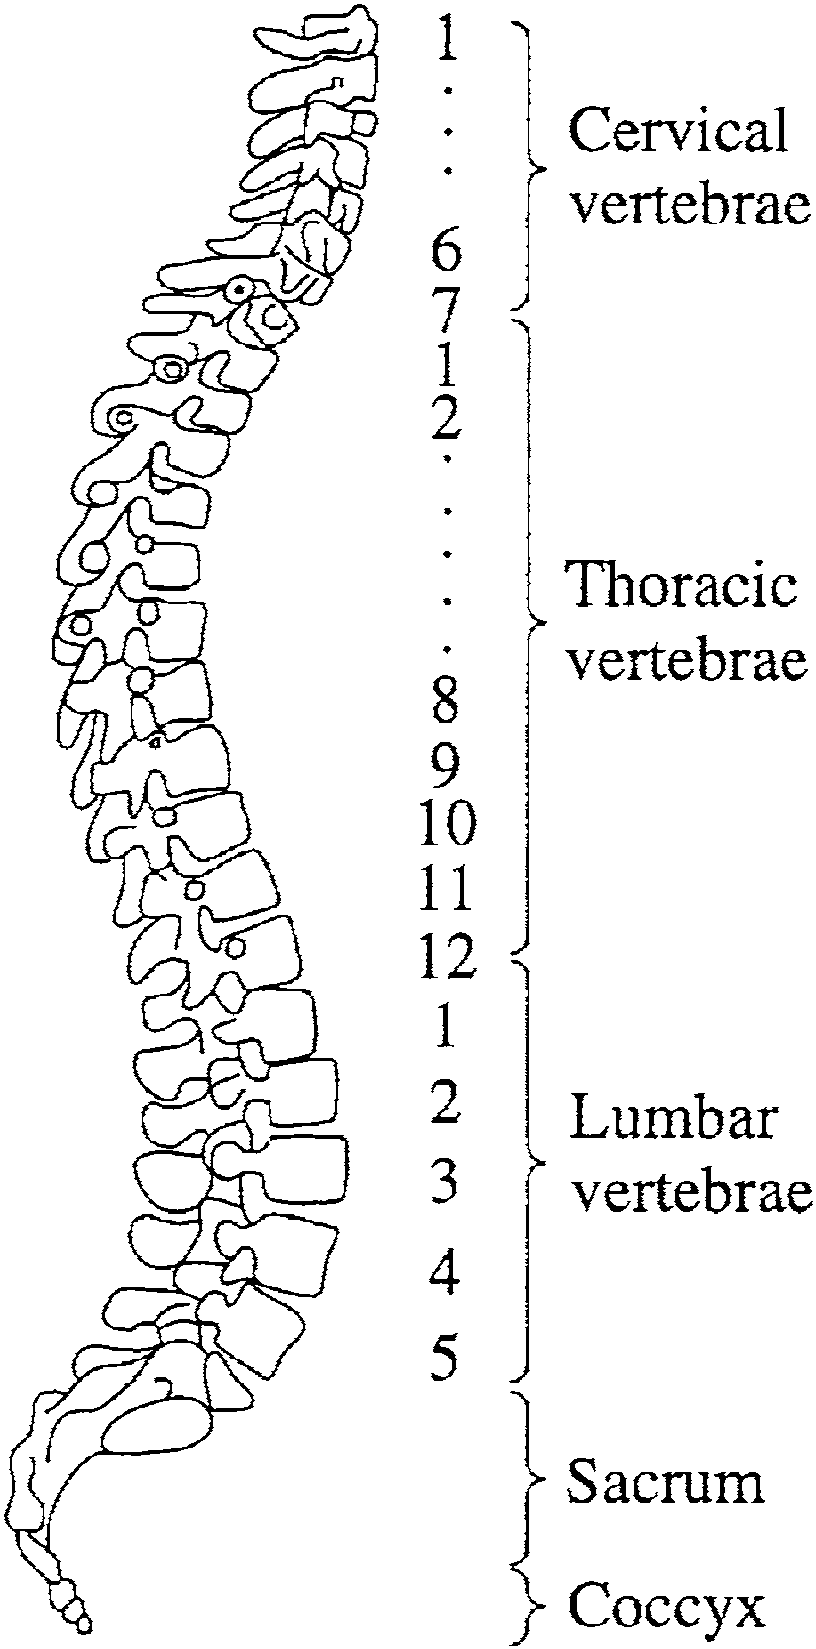
\includegraphics[width=0.5\textwidth]{234.png}
  \caption{La columna vertebral (espina). (De \cite{3}). Las curvas torácica y sacra son curvas primarias, mientras que las curvas cervical y lumbar son curvas secundarias. Las vértebras se etiquetan con la primera letra del nombre de la curva y sus números, como L1, L2, L3, L4 y L5 para las cinco vértebras lumbares.}
  \label{fig:234}
\end{SCfigure}

\begin{figure}[htbp]

  \centering
  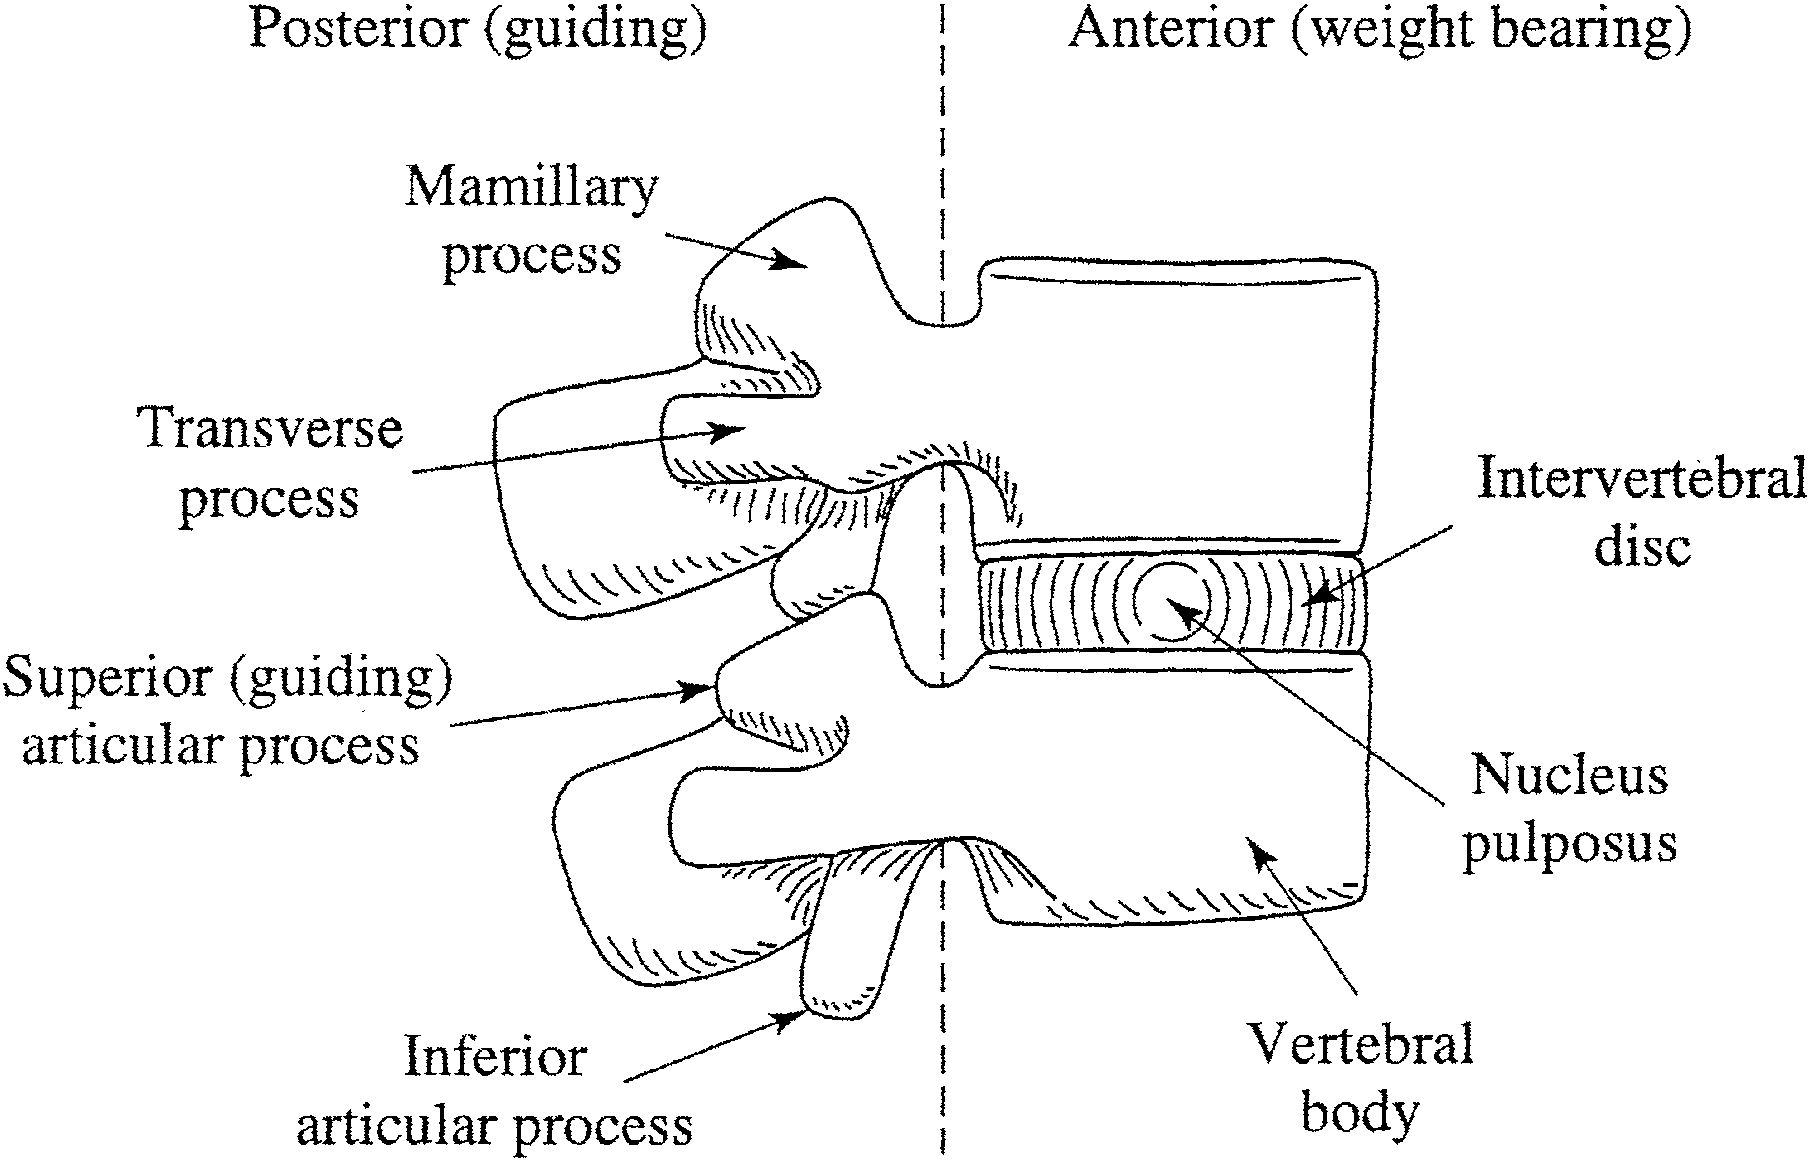
\includegraphics[width=0.75\textwidth]{235.png}
  \caption{Vista lateral de dos vértebras separadas por un disco vertebral. (De \cite{3}).}
  \label{fig:235}
\end{figure}

\begin{figure}[htbp]

  \centering
  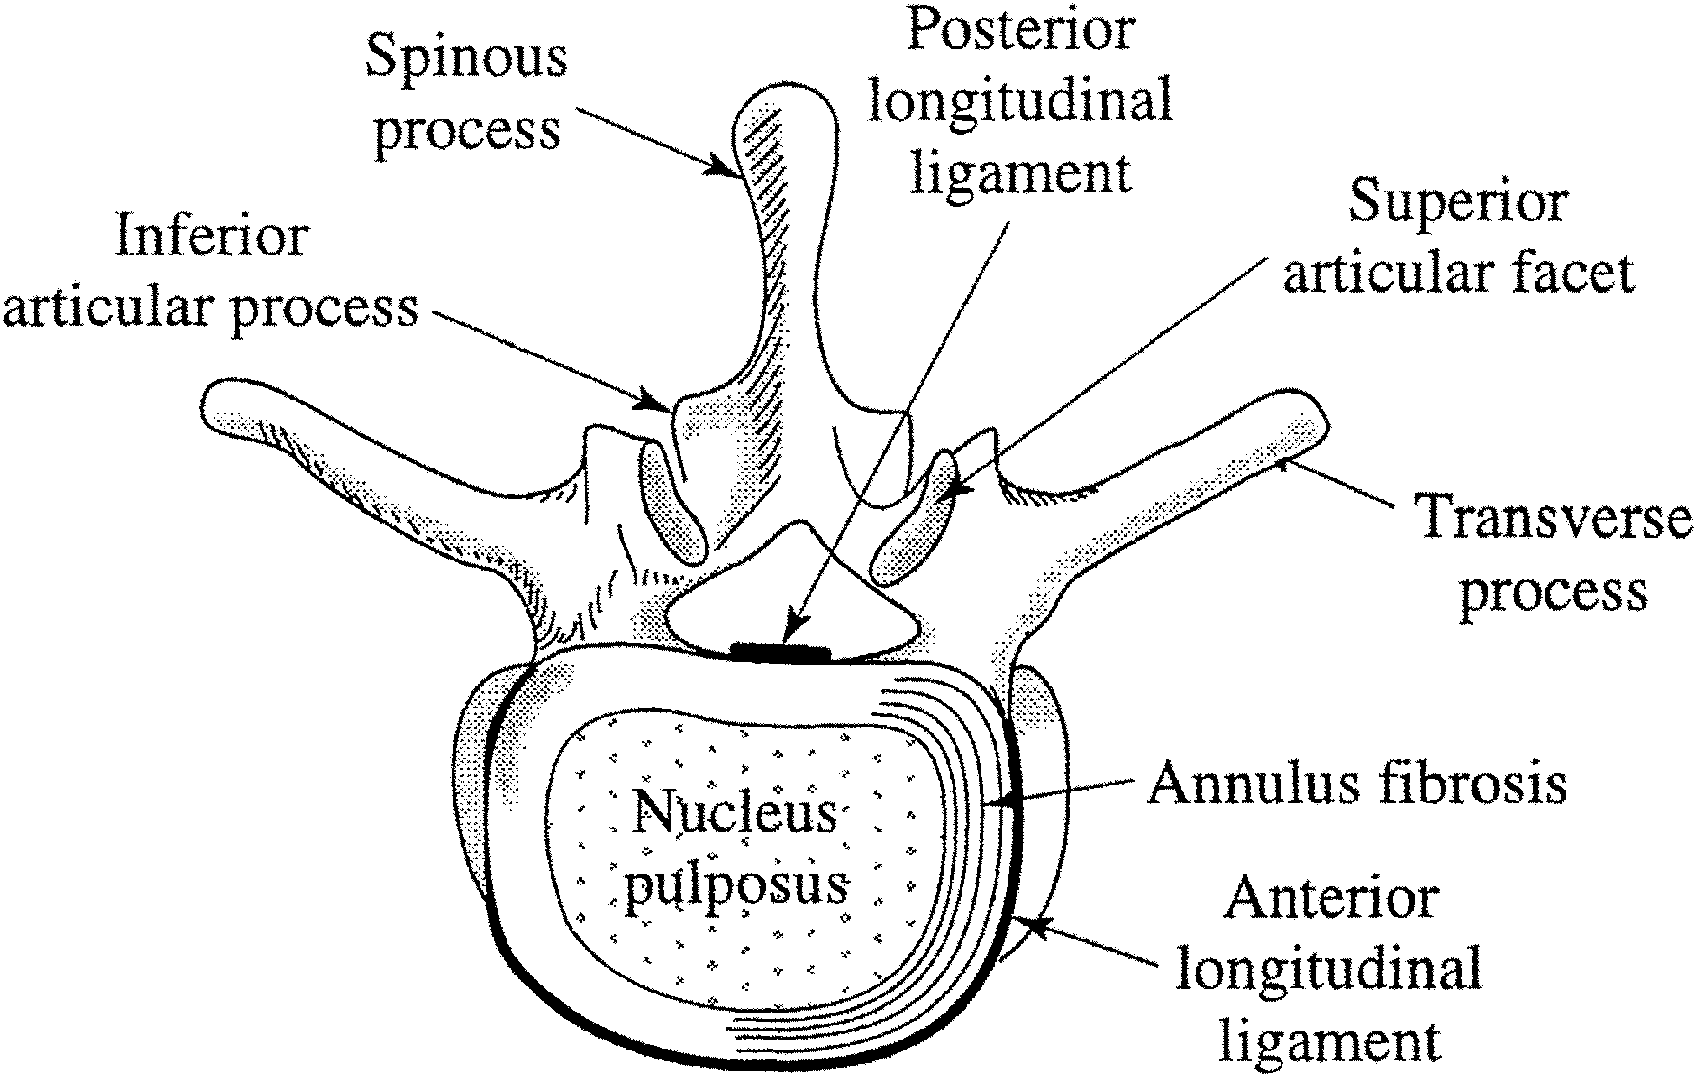
\includegraphics[width=0.7\textwidth]{236.png}
  \caption{Vértebra vista desde arriba. (De \cite{3}).}
  \label{fig:236}
\end{figure}

\begin{figure}[htbp]

  \centering
  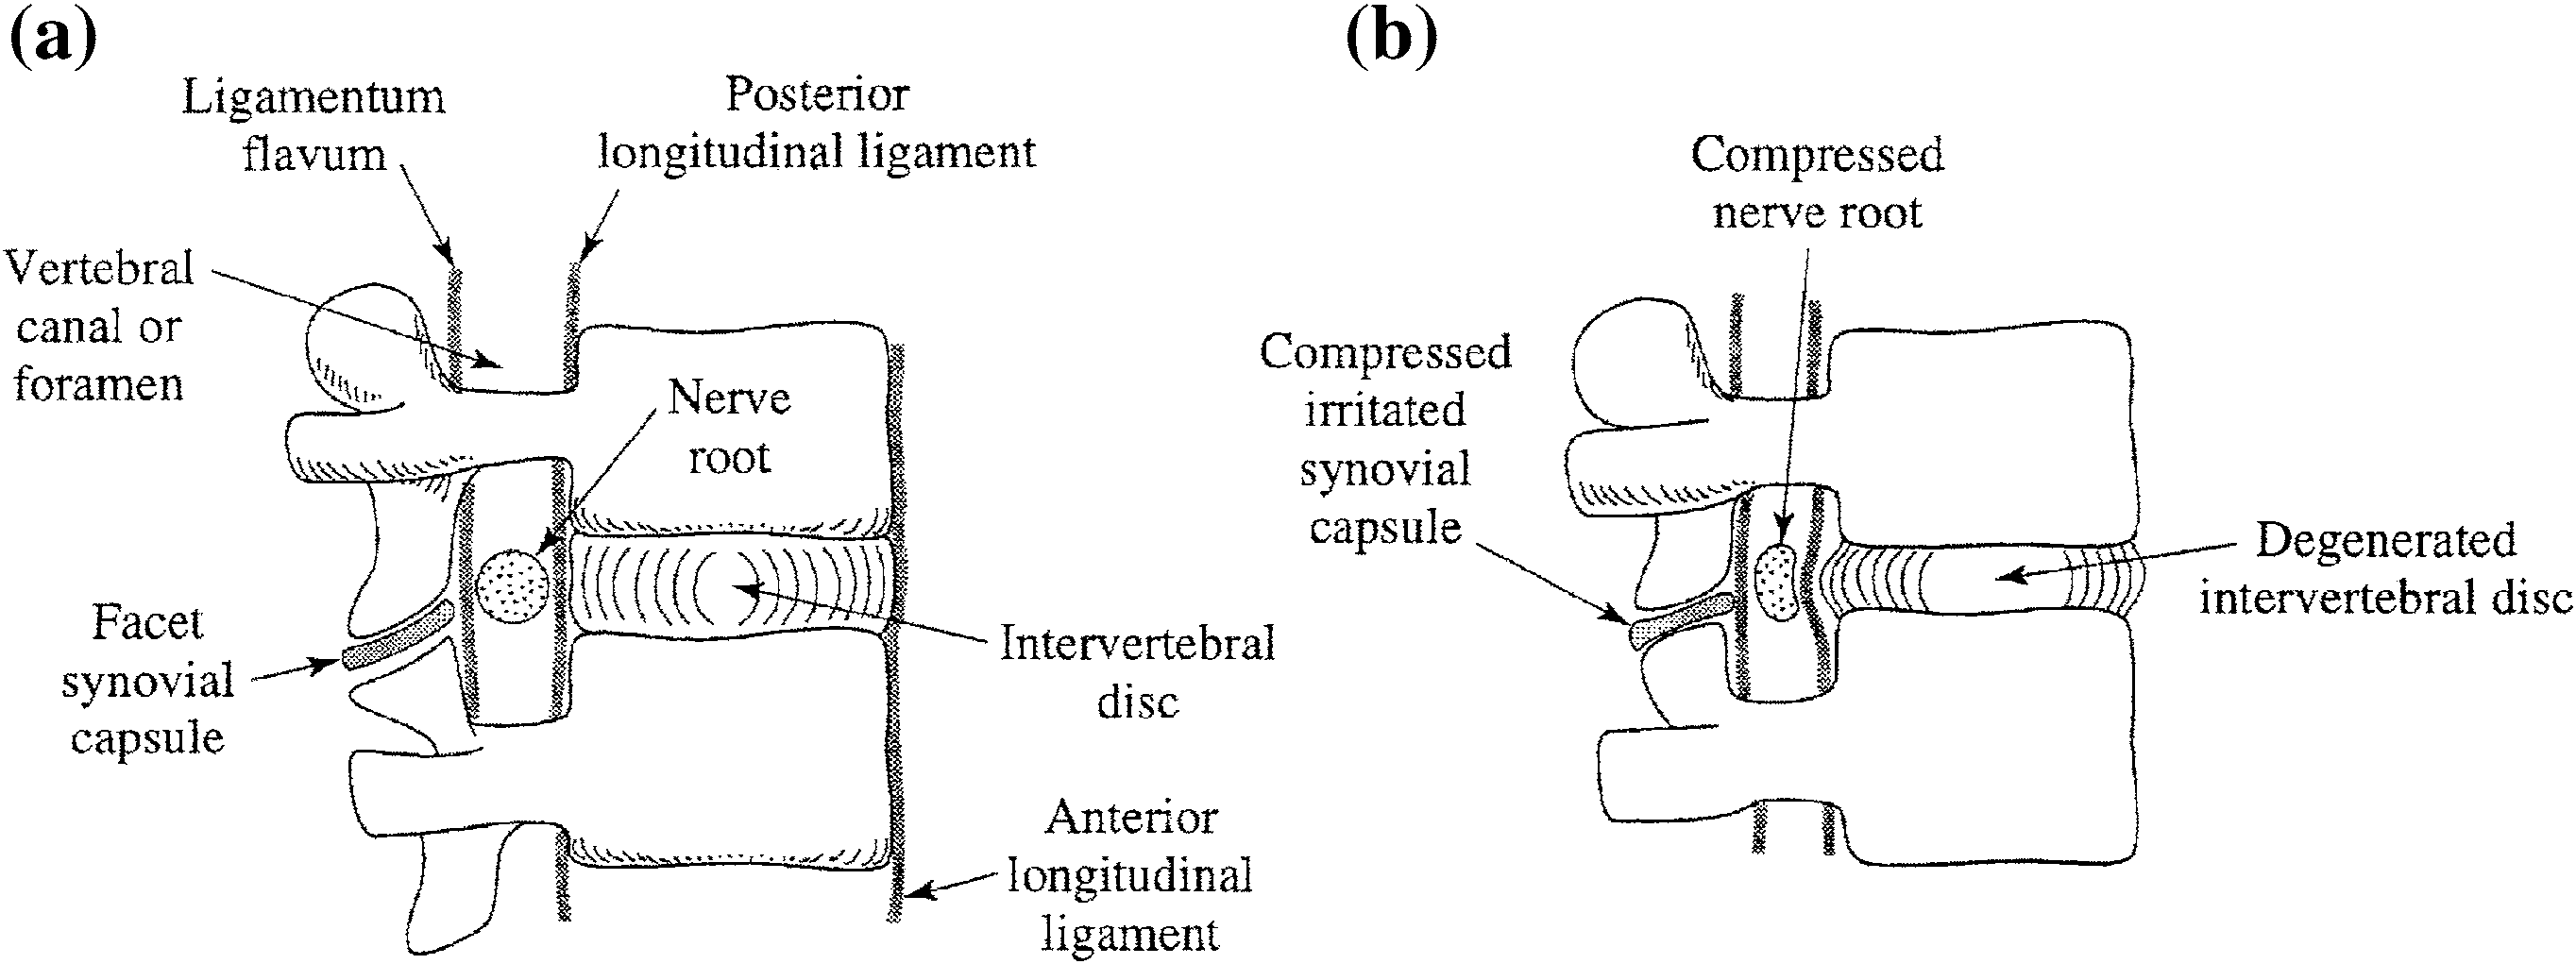
\includegraphics[width=0.75\textwidth]{237.png}
  \caption{Sección transversal de dos vértebras y un disco vertebral con nervio para \textbf{a} un disco intervertebral normal y \textbf{b} uno que se ha degenerado y está comprimiendo la raíz del nervio. (De \cite{3}).}
  \label{fig:237}
\end{figure}

 La Figura 2.38 muestra el ángulo lumbosacro entre la quinta vértebra lumbar y el sacro. Las desviaciones en el ángulo con respecto a $\sim 30^\circ$ pueden provocar dolor en la parte baja de la espalda. Modelaremos la columna vertebral como una barra rígida, a pesar de que esta descripción de las curvas de la columna sugeriría un modelo más complejo.

Existe una serie de músculos masivos desde las partes posteriores de la cresta ilíaca y el sacro hasta el cráneo (hueso occipital) llamados erectores de la columna (\textit{erector spinae}, pronunciado «es-pi'-ne») (o sacroespinales (\textit{sacrospinalis}, pronunciado «sae-kro-es-pi-na'-lis»)) (Figs. 2.39 y 2.40). Los modelaremos como un solo músculo insertado a las dos terceras partes ($2/3$) de la distancia desde el centro de masa de la cabeza y los brazos, a un ángulo de $12^\circ$ (Fig. 2.41).

\begin{figure}[htbp]

  \centering
  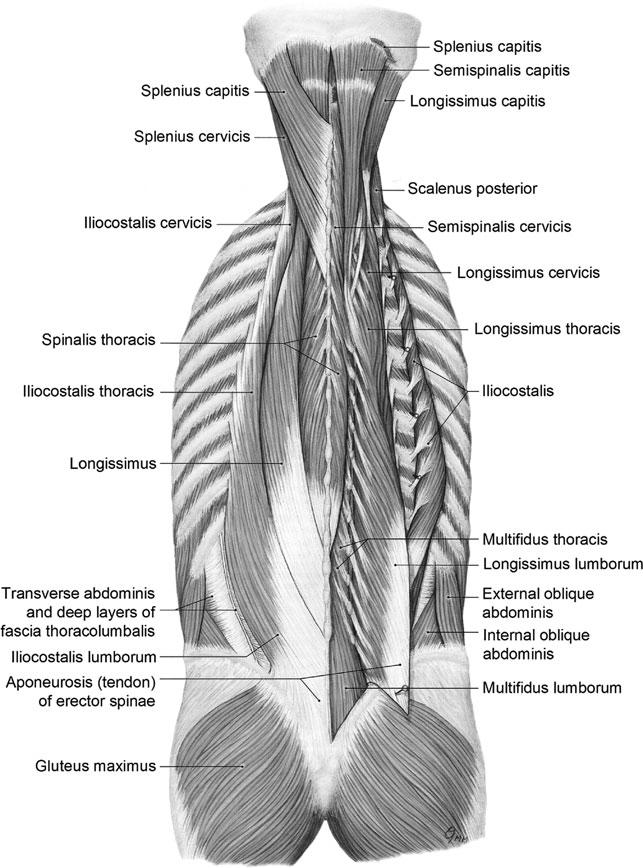
\includegraphics[width=0.55\textwidth]{239.png}
  \caption{Capas intermedia (izquierda) y profunda (derecha) de los músculos de la espalda, mostrando los músculos erectores de la columna. El erector de la columna consta de columnas laterales (los músculos iliocostal lumbar, torácico y cervical), columnas intermedias (los músculos longísimo torácico, cervical y de la cabeza) y una columna medial (espinal torácico). (De \cite{35}).}
  \label{fig:239}
\end{figure}

\begin{SCfigure}[0.5][htbp]

  \centering
  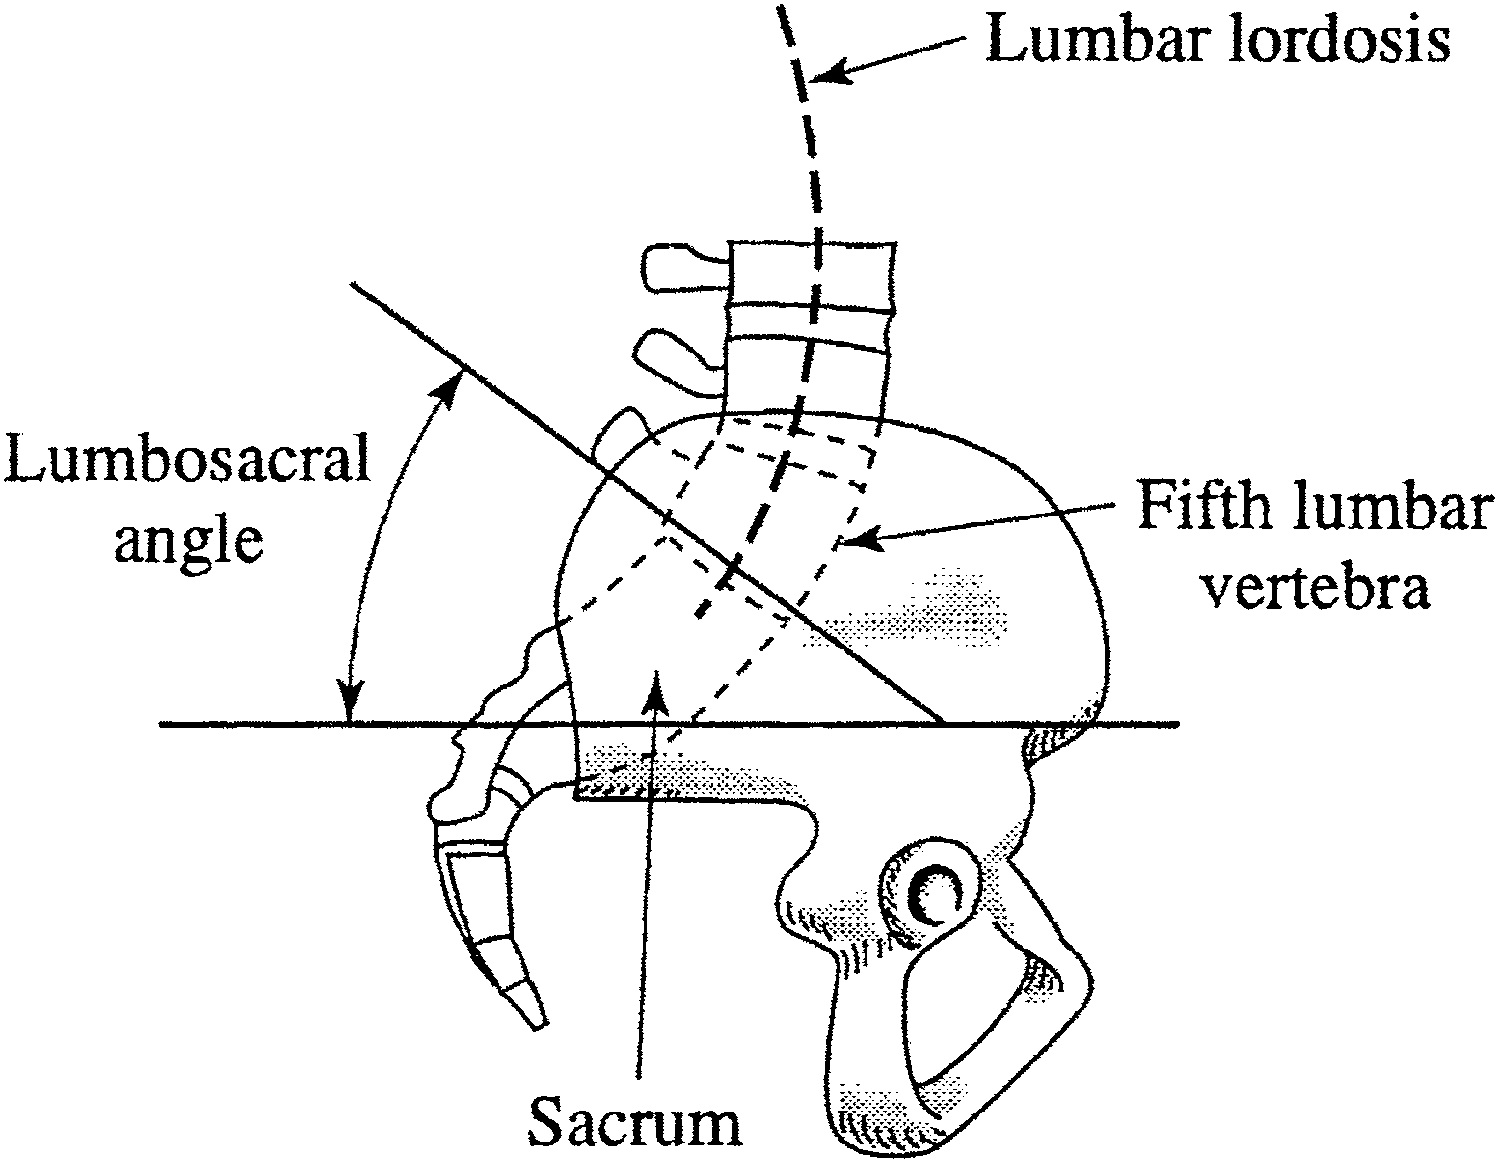
\includegraphics[width=0.5\textwidth]{240.png}
  \caption{Diagrama de los músculos erectores de la columna utilizados para controlar el tronco al inclinarse. (De \cite{3}).}
  \label{fig:240}
\end{SCfigure}



Considere la columna vertebral a un ángulo $\theta$ con respecto a la horizontal (Fig. 2.41); inicialmente tomaremos $\theta = 30^\circ$, lo que corresponde a una flexión profunda. Está articulada en el disco lumbosacro, justo debajo de la quinta vértebra lumbar y por encima del sacro (Figs. 2.38 y 2.41). Elegiremos el eje para el análisis de torque justo allí.

\begin{SCfigure}[0.5][htbp]

  \centering
  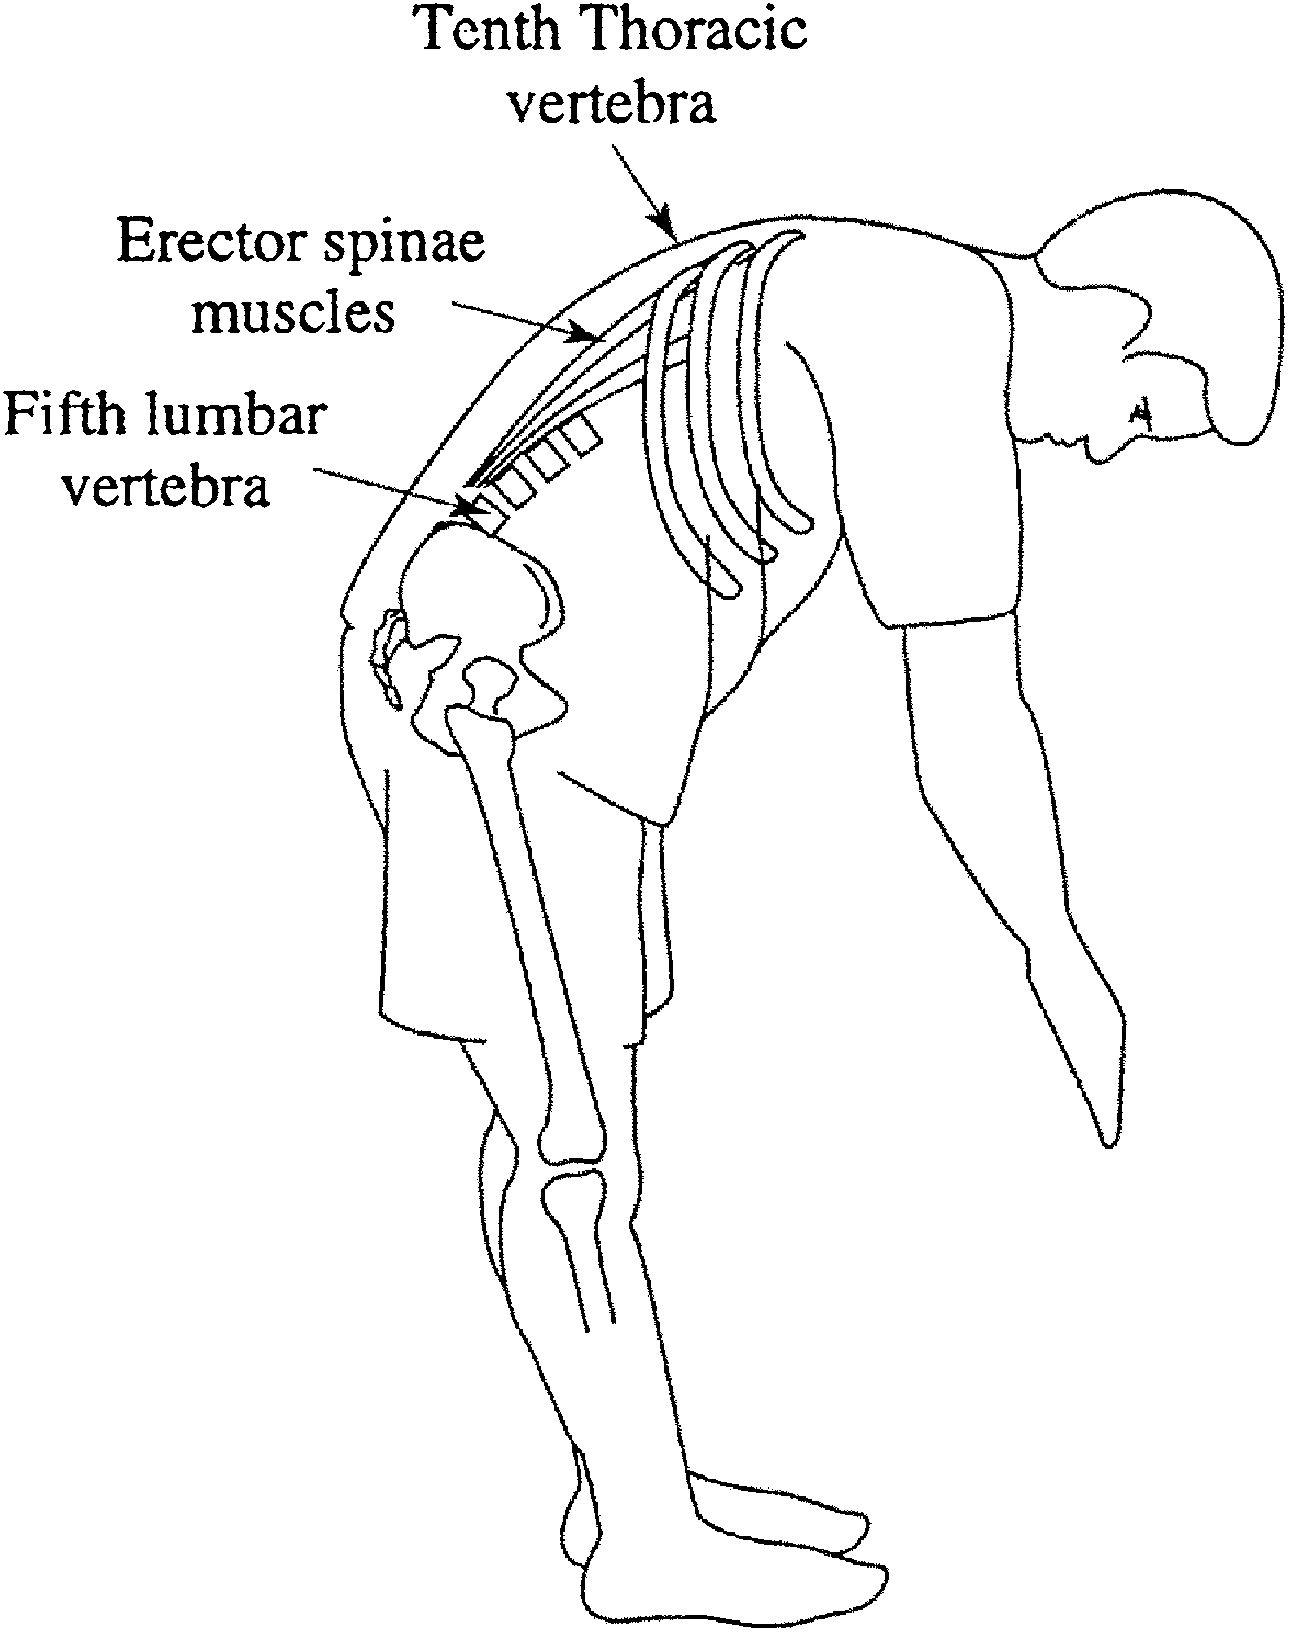
\includegraphics[width=0.55\textwidth]{238.png}
  \caption{El ángulo lumbosacro se define como el que existe entre la horizontal y la superficie superior del sacro. (De \cite{3}).}
  \label{fig:238}
\end{SCfigure}

 Hay una fuerza de reacción $\vec{\mathbf{R}}$ (de magnitud $R$) desde el sacro con componentes $R_x$ y $R_y$. El peso del tronco (por encima de las caderas, excluyendo los brazos y la cabeza) $W_1$ actúa a la mitad de la columna vertebral. El peso de los brazos, la cabeza y cualquier objeto levantado, $W_2$, actúan en la parte superior de la columna vertebral. Estos se muestran en la Fig. 2.41 junto con la fuerza del erector de la columna $\vec{\mathbf{M}}$ (de magnitud $M$). Utilizando la Tabla 1.7, es razonable aproximar $W_1 = 0,4 W_b$ y $W_2 = 0,2 W_b$, sin levantar nada.

\begin{SCfigure}[0.5][htbp]

  \centering
  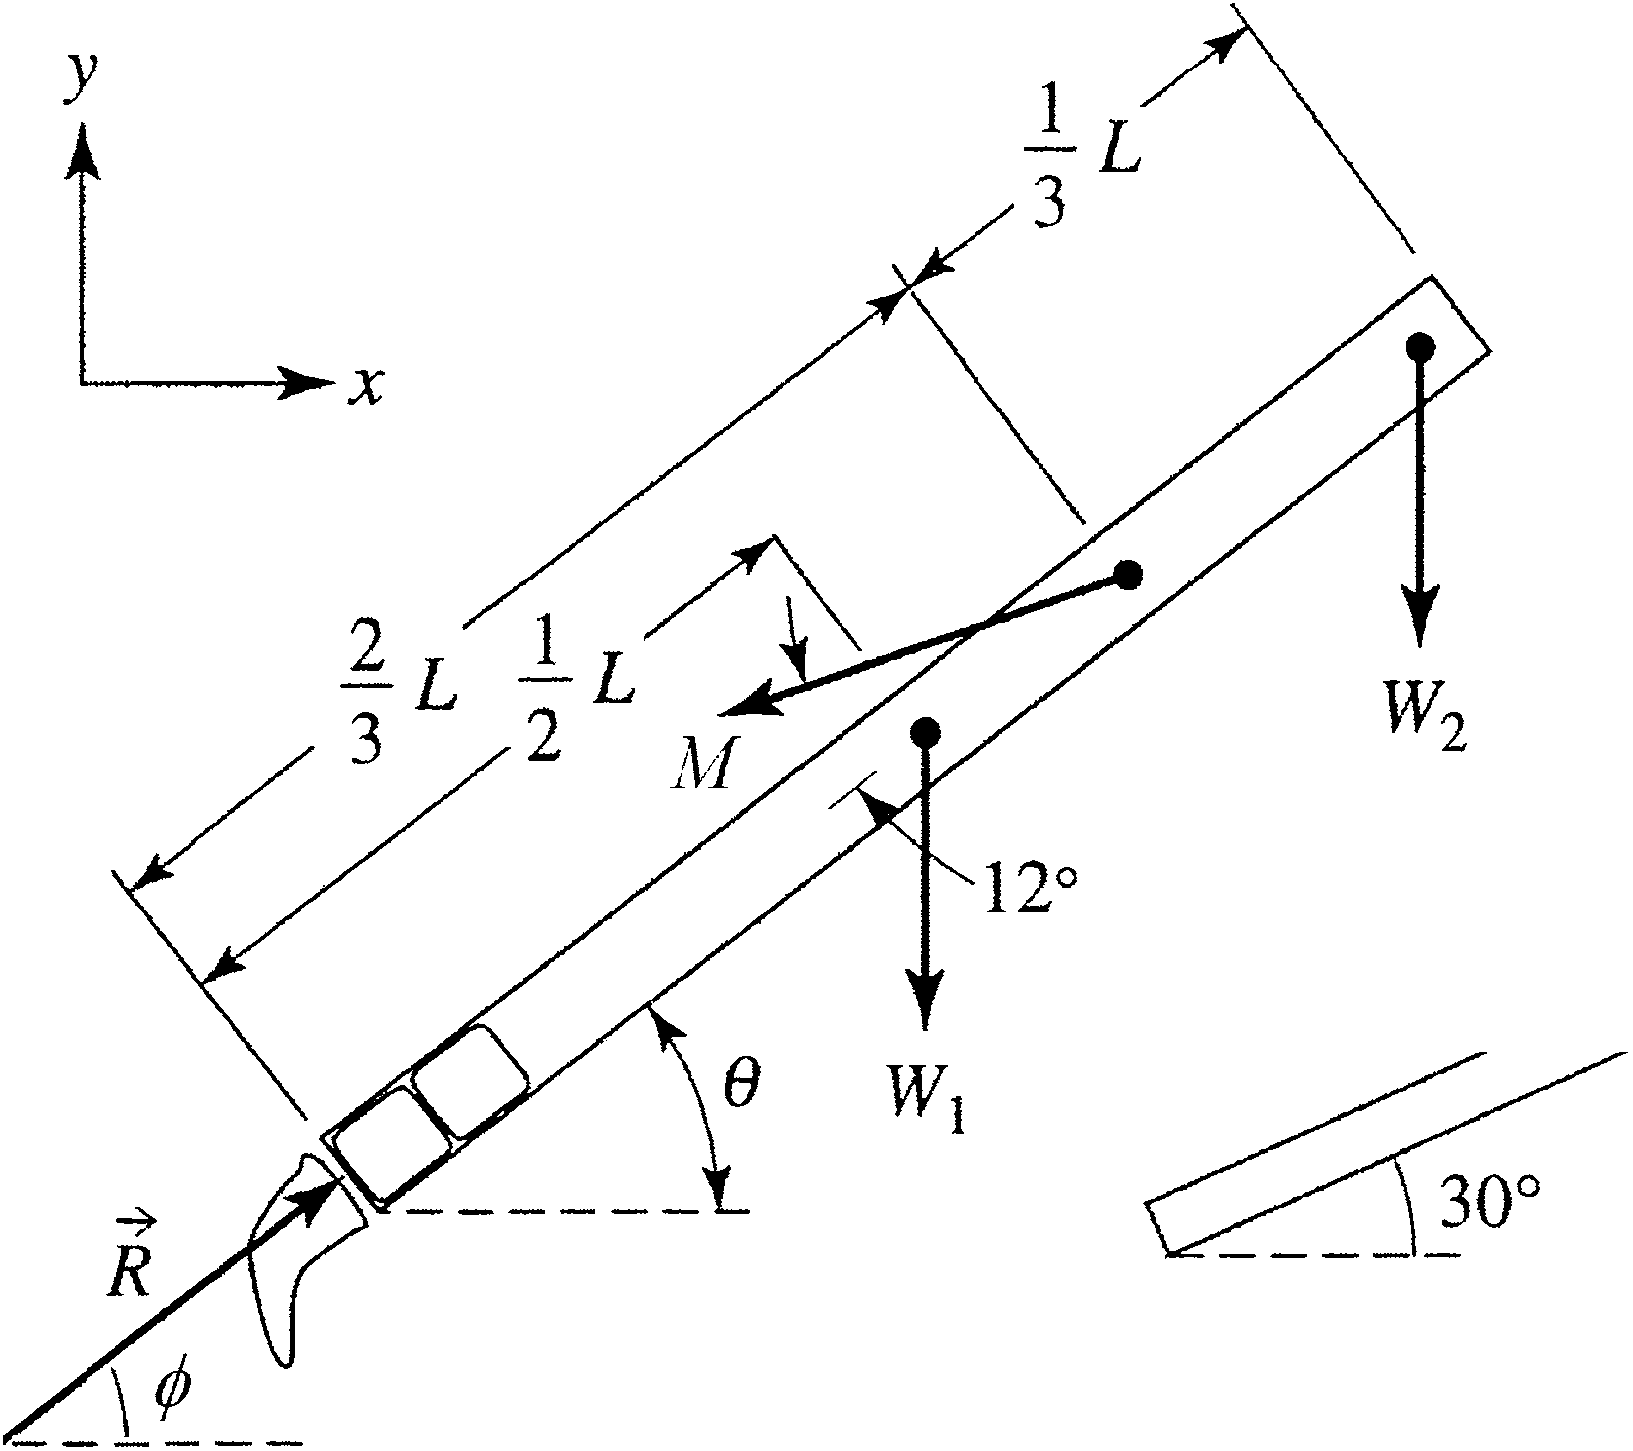
\includegraphics[width=0.55\textwidth]{241.png}
  \caption{Diagrama de cuerpo libre de la columna vertebral al inclinarse, con la columna vertebral modelada como una barra recta a un ángulo $\theta$ con respecto a la horizontal, que tomaremos como $\sim 30^\circ$ ---una inclinación un poco más pronunciada de la que se representa aquí y se muestra en el recuadro---. El ángulo de $\vec{\mathbf{R}}$ con respecto a la horizontal es $\phi$. Sin levantar nada, tomaremos $W_1 = 0,4 W_b$ y $W_2 = 0,2 W_b$. (De \cite{3}).}
  \label{fig:241}
\end{SCfigure}



La Figura 2.41 muestra que $\vec{\mathbf{M}}$ actúa a un ángulo que es $\theta - 12^\circ$ con respecto a la horizontal; para nuestro primer ejemplo, $\theta = 30^\circ$ y por lo tanto este ángulo es $18^\circ$. Los balances de fuerzas son
\begin{equation}
F_x = R_x - M \cos 18^\circ = 0,
\label{eq:2.41}
\end{equation}
\begin{equation}
F_y = R_y - M \sin 18^\circ - 0,4 W_b - 0,2 W_b = 0.
\label{eq:2.42}
\end{equation}

Con esta elección del eje de rotación, el torque debido a la fuerza de reacción es cero. La componente de $M$ normal a la columna vertebral es $F' = M \sin 12^\circ$, lo que conduce a un torque de $(2L/3)(\sin 12^\circ)(M)$. La fracción de cada fuerza de peso normal a la columna vertebral es $\cos \theta = \cos 30^\circ$. El equilibrio de torque requiere
\begin{equation}
\tau_z = \frac{2L}{3} \sin 12^\circ (M) - \frac{L}{2} \cos 30^\circ (0,4 W_b) - L \cos 30^\circ (0,2 W_b) = 0.
\label{eq:2.43}
\end{equation}

La ecuación de torque da $M = 2,5 W_b$ o $2200\text{ N}$ (500 lb) para el peso corporal de $880\text{ N}$ (200 lb) de una masa corporal de $90\text{ kg}$. Los parámetros de la fuerza de reacción son $R_x = M \cos 18^\circ = 2,38 W_b$, $R_y = 1,37 W_b$, $\phi = \arctan(R_y/R_x) = 30^\circ$ (que es el ángulo que la fuerza de reacción forma con la horizontal) y $R = 2,74 W_b$, que es $2400\text{ N}$ (540 lb) aquí. Claramente, las fuerzas musculares y la fuerza de reacción en la parte inferior de la columna vertebral son mucho mayores que el peso corporal. Los brazos de momento de los pesos son aproximadamente los mismos que el del músculo. Sin embargo, la dirección de las fuerzas de peso conduce a grandes torques con ángulos de flexión grandes, mientras que la dirección de la fuerza muscular no conduce a un torque grande para equilibrar los pesos ---a cualquier ángulo de flexión---.

Las cosas son aun peores si sostiene un peso en sus brazos; esto simula doblar la espalda y levantar un objeto de este peso. Todo lo que esto hace es aumentar $W_2$. Aumentemos $W_2$ en $0,2 W_b$ ($180\text{ N}$ (40 lb) en nuestro ejemplo) a $0,4 W_b$. Ahora
\begin{equation}
F_x = R_x - M \cos 18^\circ = 0,
\label{eq:2.44}
\end{equation}
\begin{equation}
F_y = R_y - M \sin 18^\circ - 0,4 W_b - 0,4 W_b = 0,
\label{eq:2.45}
\end{equation}
\begin{equation}
\tau_z = \frac{2L}{3} \sin 12^\circ (M) - \frac{L}{2} \cos 30^\circ (0,4 W_b) - L \cos 30^\circ (0,4 W_b) = 0.
\label{eq:2.46}
\end{equation}

La fuerza que los músculos erectores de la columna necesitan ejercer aumenta a $3,74 W_b$ o $3300\text{ N}$ (740 lb). Los músculos deben ejercer $1100\text{ N}$ (250 lb) adicionales para equilibrar solo $180\text{ N}$ (40 lb) adicionales. Vemos que $R_x = 3,56 W_b$, $R_y = 1,96 W_b$ y $R = 4,07 W_b$. Esto es $3600\text{ N}$ (810 lb), lo que representa una fuerza de reacción adicional de $1200\text{ N}$ (270 lb) sobre la quinta vértebra lumbar.

La Tabla 2.3 muestra estas fuerzas para varios ángulos de flexión. Podemos ver por qué la flexión en sí misma, y la flexión junto con el levantamiento, pueden provocar problemas con los músculos de la espalda y con los discos vertebrales inferiores.

\begin{table}[htbp]
\centering
\caption{Fuerzas en la columna vertebral durante la flexión y el levantamiento.}
\label{tab:23}
\begin{tabularx}{0.8\textwidth}{l>{\centering\arraybackslash}X>{\centering\arraybackslash}X>{\centering\arraybackslash}X>{\centering\arraybackslash}X}
\toprule
$\theta$ & $M$ (sin levantar) & $M$ ($0,2 W_b$ extra) & $R$ (sin levantar) & $R$ ($0,2 W_b$ extra) \\
\midrule
$30^\circ$ & 2,50 & 3,74 & 2,74 & 4,07 \\
$60^\circ$ & 1,44 & 2,16 & 1,93 & 2,81 \\
$80^\circ$ & 0,50 & 0,75 & 1,08 & 1,53 \\
$90^\circ$ & 0 & 0 & 0,60 & 0,80 \\
\bottomrule
\end{tabularx}
\begin{flushleft}
    \small Todas las fuerzas están en unidades del peso corporal. Para una masa corporal de 90 kg, multiplique cada número por 880 N (200 lb).
\end{flushleft}
\end{table}

¿Qué significa esto para el disco lumbosacro (intervertebral)? Consideremos nuestro ejemplo inicial de inclinación de $60^\circ$ desde la posición erguida, hasta $30^\circ$ desde la horizontal, sin levantar ningún peso. La fuerza de reacción sobre este disco es de $2400\text{ N}$ (540 lb). Esta fuerza empuja hacia abajo en la parte superior y hacia arriba en la parte inferior de este disco cilíndrico. Estamos asumiendo una carga que es normal al eje, lo cual no es exactamente correcto a estos ángulos.

\begin{SCfigure}[0.5][htbp]

  \centering
  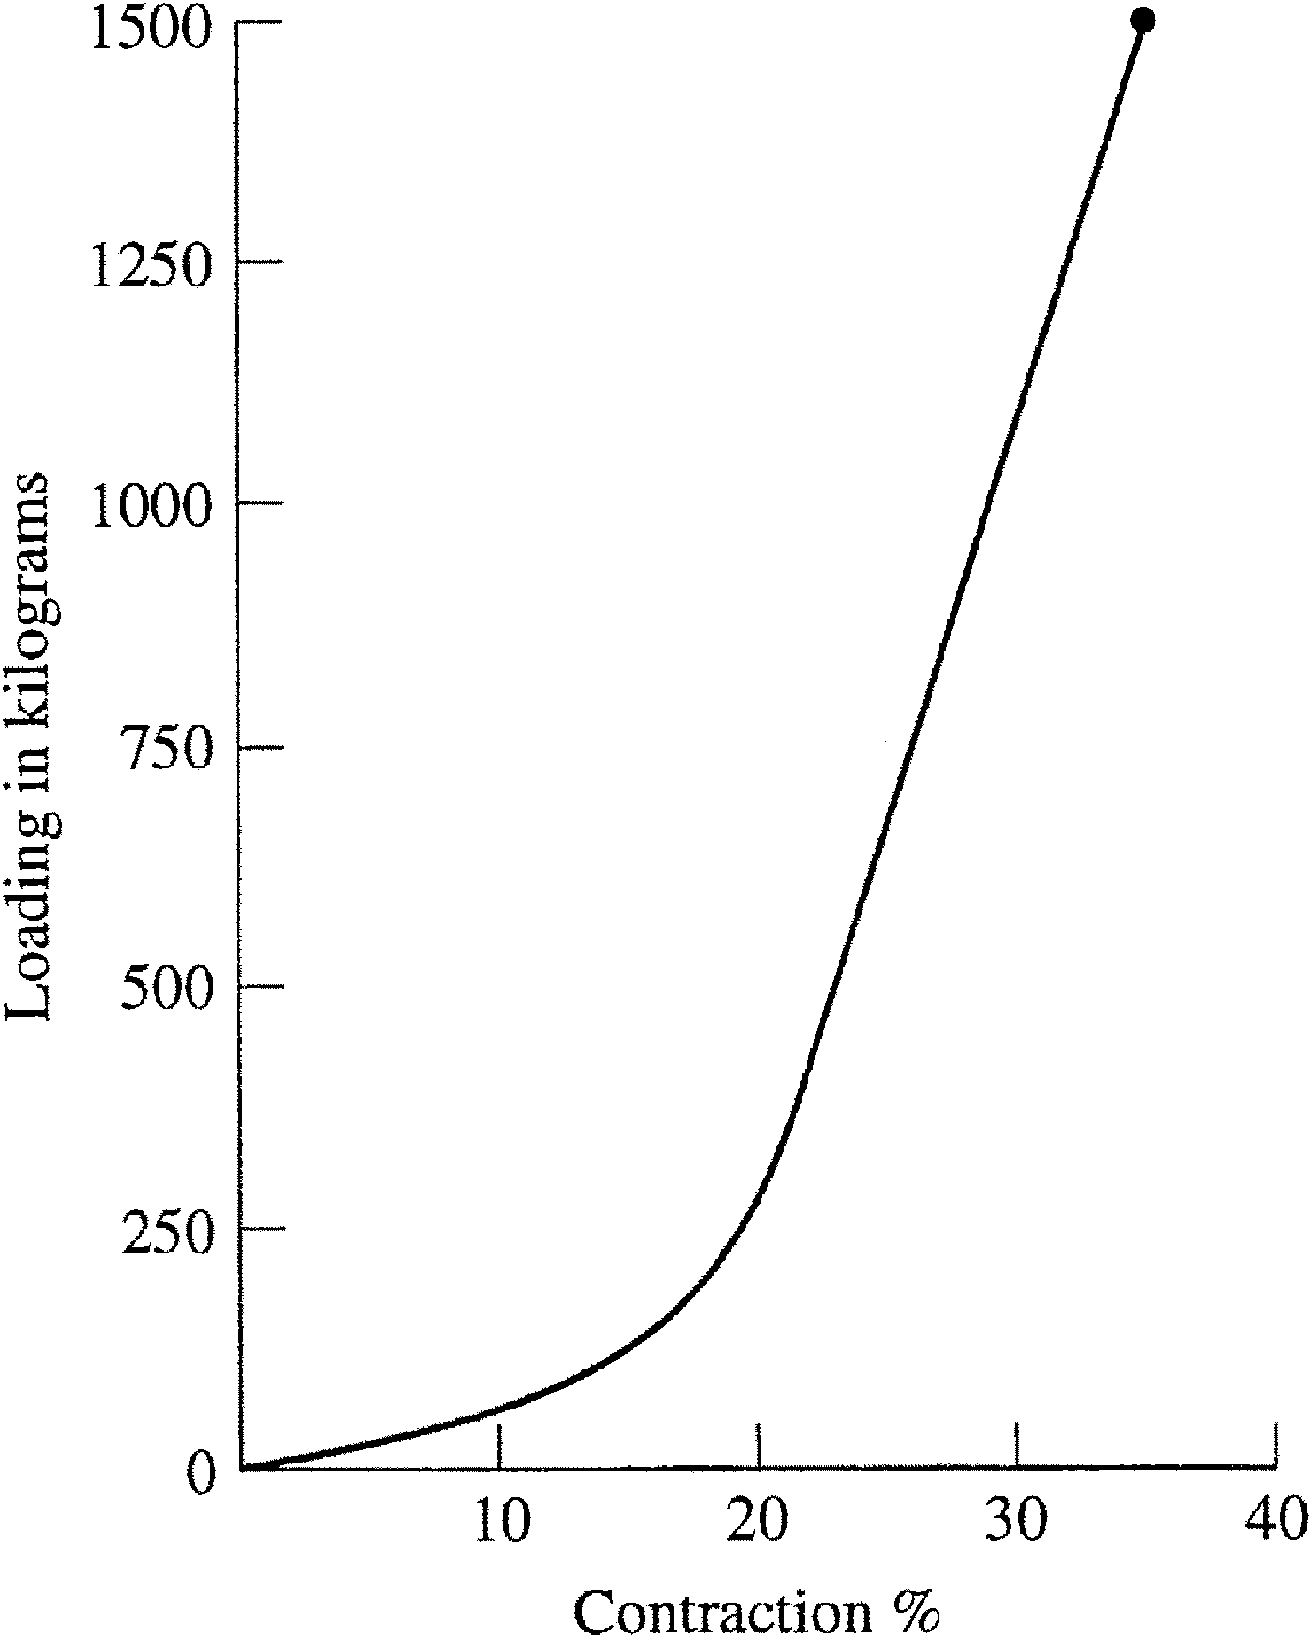
\includegraphics[width=0.5\textwidth]{242.png}
  \caption{Carga de discos vertebrales lumbares húmedos de personas de 40 a 59 años de edad versus porcentaje de compresión. Para la carga en N, la escala de la ordenada debe multiplicarse por 9,8. (De \cite{3}. Basado en \cite{40}).}
  \label{fig:242}
\end{SCfigure}

 La Figura 2.42 muestra cuánto disminuye fraccionalmente la altura del disco con este tipo de carga. El peso correspondiente a $250\text{ kg}$ es de $2400\text{ N}$ (540 lb), por lo que usando esta figura se espera una contracción del 20\% paralela a la columna. Si el disco es un cilindro de radio $r$ y altura $H$, entonces su volumen es $\pi r^2 H$. Si el material del disco es incompresible, su volumen no cambiará con esta compresión y, si $H$ disminuye en un 20\%, $r$ aumentará en aproximadamente un 10\%. El disco protuberante (o hernia discal) puede presionar contra el nervio, como se ve en la Fig. 2.37b. Al levantar peso, la fuerza de reacción aumenta aún más, la compresión del disco se incrementa y hay una mayor protuberancia y mayor irritación de los nervios.

Acabamos de comparar una carga de $245\text{ kg}$ ($2400\text{ N}$, 540 lb) sobre el disco con una situación sin fuerza sobre este disco. En la posición erguida, ya hay $0,6 \times$ la masa corporal (y el peso), es decir, $54\text{ kg}$ ($530\text{ N}$, 120 lb) soportados por este disco debido al peso corporal, por lo que la carga realmente cambia de $530\text{ N}$ (120 lb) a $2400\text{ N}$ (540 lb). (¿Cómo afecta esto a nuestros resultados numéricos y conclusiones?). Además, la carga no es uniforme cuando se levanta peso o se dobla la espalda, y debido a esto puede haber tensión, compresión y protuberancia, como en la Fig. 2.43.

\begin{figure}[htbp]

  \centering
  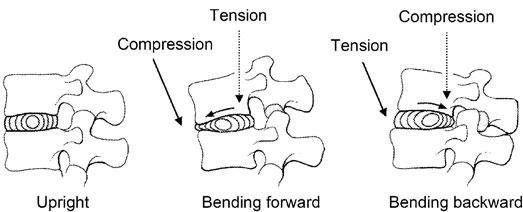
\includegraphics[width=0.7\textwidth]{243.png}
  \caption{Compresión del disco para una persona que está \textbf{a} vertical, \textbf{b} inclinada hacia adelante y \textbf{c} inclinada hacia atrás. Inclinarse hacia adelante conduce a la compresión del disco en la parte anterior y tensión en la parte posterior, protuberancia en el lado compresivo y el desplazamiento del núcleo del disco hacia la parte posterior. (De \cite{30}).}
  \label{fig:243}
\end{figure}



Esto nos enseña dos cosas. (1) Comprender las propiedades mecánicas de las partes del cuerpo es esencial para entender las implicaciones de las fuerzas sobre el cuerpo; las examinaremos en el Cap. 4. (2) Nunca se debe doblar la espalda y levantar peso. Los Problemas 2.34 a 2.36 examinan los torques durante el levantamiento de objetos de diferentes tamaños, con diferentes posiciones del cuerpo superior (como arriba) y con diferentes técnicas.

Estas fuerzas en la parte baja de la espalda dependen no solo del ángulo de la columna y de la carga, sino de la flexión de las rodillas durante el levantamiento y de dónde está posicionada la carga con respecto al cuerpo. Al estar acostado, las fuerzas en la parte baja de la espalda son del 20 al 50\% de aquellas al estar de pie erguido y relajado (Tabla 2.4), y alcanzan valores de más del doble del peso corporal y de más de $3\times$ el peso del torso durante la marcha rápida (Fig. 2.44).

\begin{figure}[htbp]

  \centering
  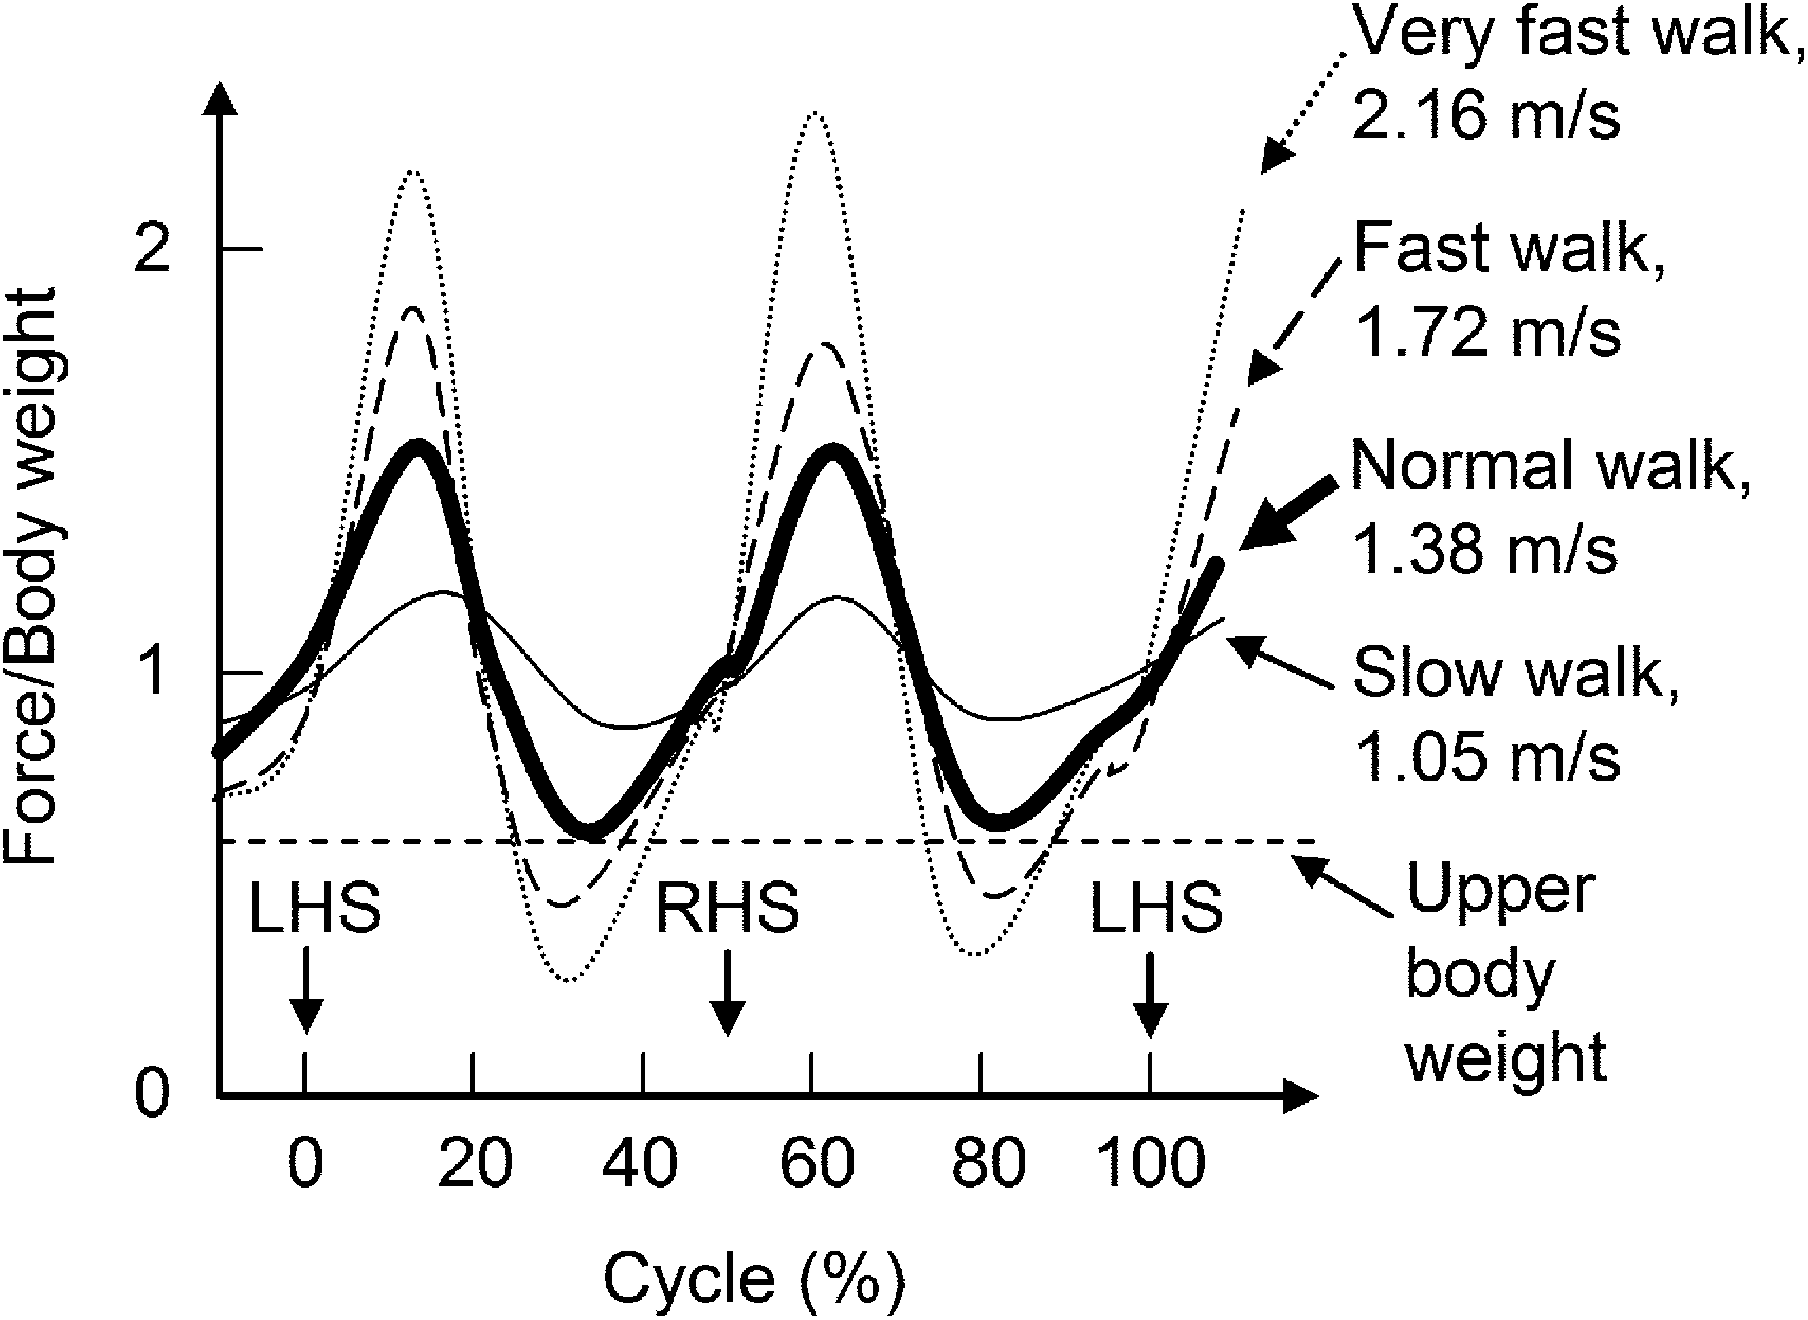
\includegraphics[width=0.75\textwidth]{244.png}
  \caption{Carga axial sobre el disco entre las vértebras L3 y L4 al caminar a diferentes velocidades. LHS y RHS son el contacto del talón izquierdo y derecho, respectivamente. (Basado en \cite{6, 25}).}
  \label{fig:244}
\end{figure}

 La Tabla 2.4 muestra que la presión entre los discos vertebrales para las personas sentadas se minimiza cuando se encorvan, por lo que cuando sus padres u otras personas les digan que dejen de encorvarse, pueden responder que están tratando de minimizar la presión intradiscal para el cuidado a largo plazo de su columna vertebral.

\begin{table}[htbp]
\centering
\caption{Valores de presión intradiscal para diferentes posiciones y ejercicios, en relación con la presión durante la bipedestación relajada.}
\label{tab:24}
\begin{tabularx}{0.8\textwidth}{l>{\centering\arraybackslash}X}
\toprule
\textbf{Posición o actividad} & \textbf{\%} \\
\midrule
\multicolumn{2}{l}{\textbf{Estática}} \\
Acostado boca arriba (decúbito supino) & 20 \\
Acostado de lado & 24 \\
Acostado boca abajo (decúbito prono) & 22 \\
Acostado boca abajo, espalda extendida, apoyando los codos & 50 \\
Bipedestación relajada & 100 \\
De pie, inclinado hacia adelante & 220 \\
Sentado relajado, sin respaldo & 92 \\
Sentado enderezando activamente la espalda & 110 \\
Sentado con flexión máxima (inclinado hacia adelante) & 166 \\
Sentado inclinado hacia adelante, muslo apoyando los codos & 86 \\
Sentado encorvado en una silla & 54 \\
\midrule
\multicolumn{2}{l}{\textbf{Movimiento}} \\
Levantarse de la silla & 220 \\
Caminar descalzo o con tenis & 106--130 \\
Trotar con tenis & 70--180 \\
Subir escaleras, de una en una & 100--140 \\
Subir escaleras, de dos en dos & 60--240 \\
Bajar escaleras, de una en una & 76--120 \\
Bajar escaleras, de dos en dos & 60--180 \\
\midrule
\multicolumn{2}{l}{\textbf{Levantamiento}} \\
Levantar 20 kg, sin doblar las rodillas & 460 \\
Levantar 20 kg, rodillas dobladas, peso cerca del cuerpo & 340 \\
Sostener 20 kg cerca del cuerpo & 220 \\
Sostener 20 kg, a 60 cm del pecho & 360 \\
\bottomrule
\end{tabularx}
\begin{flushleft}
    \small Utilizando datos de \cite{22, 25, 37}
\end{flushleft}
\end{table}

¿Cómo puede mantener su espalda y aliviar el dolor lumbar si tiene un daño relativamente menor en la parte baja de la espalda? Estire los músculos de la espalda. Doble siempre las rodillas y use los músculos de las piernas (y no los de la espalda) al levantar peso. Asegúrese de mantener la curvatura de la parte baja de la espalda en todo momento. Debe sentarse en sillas con soporte lumbar (ver Fig. 2.45 y \cite{33})

\begin{figure}[htbp]

  \centering
  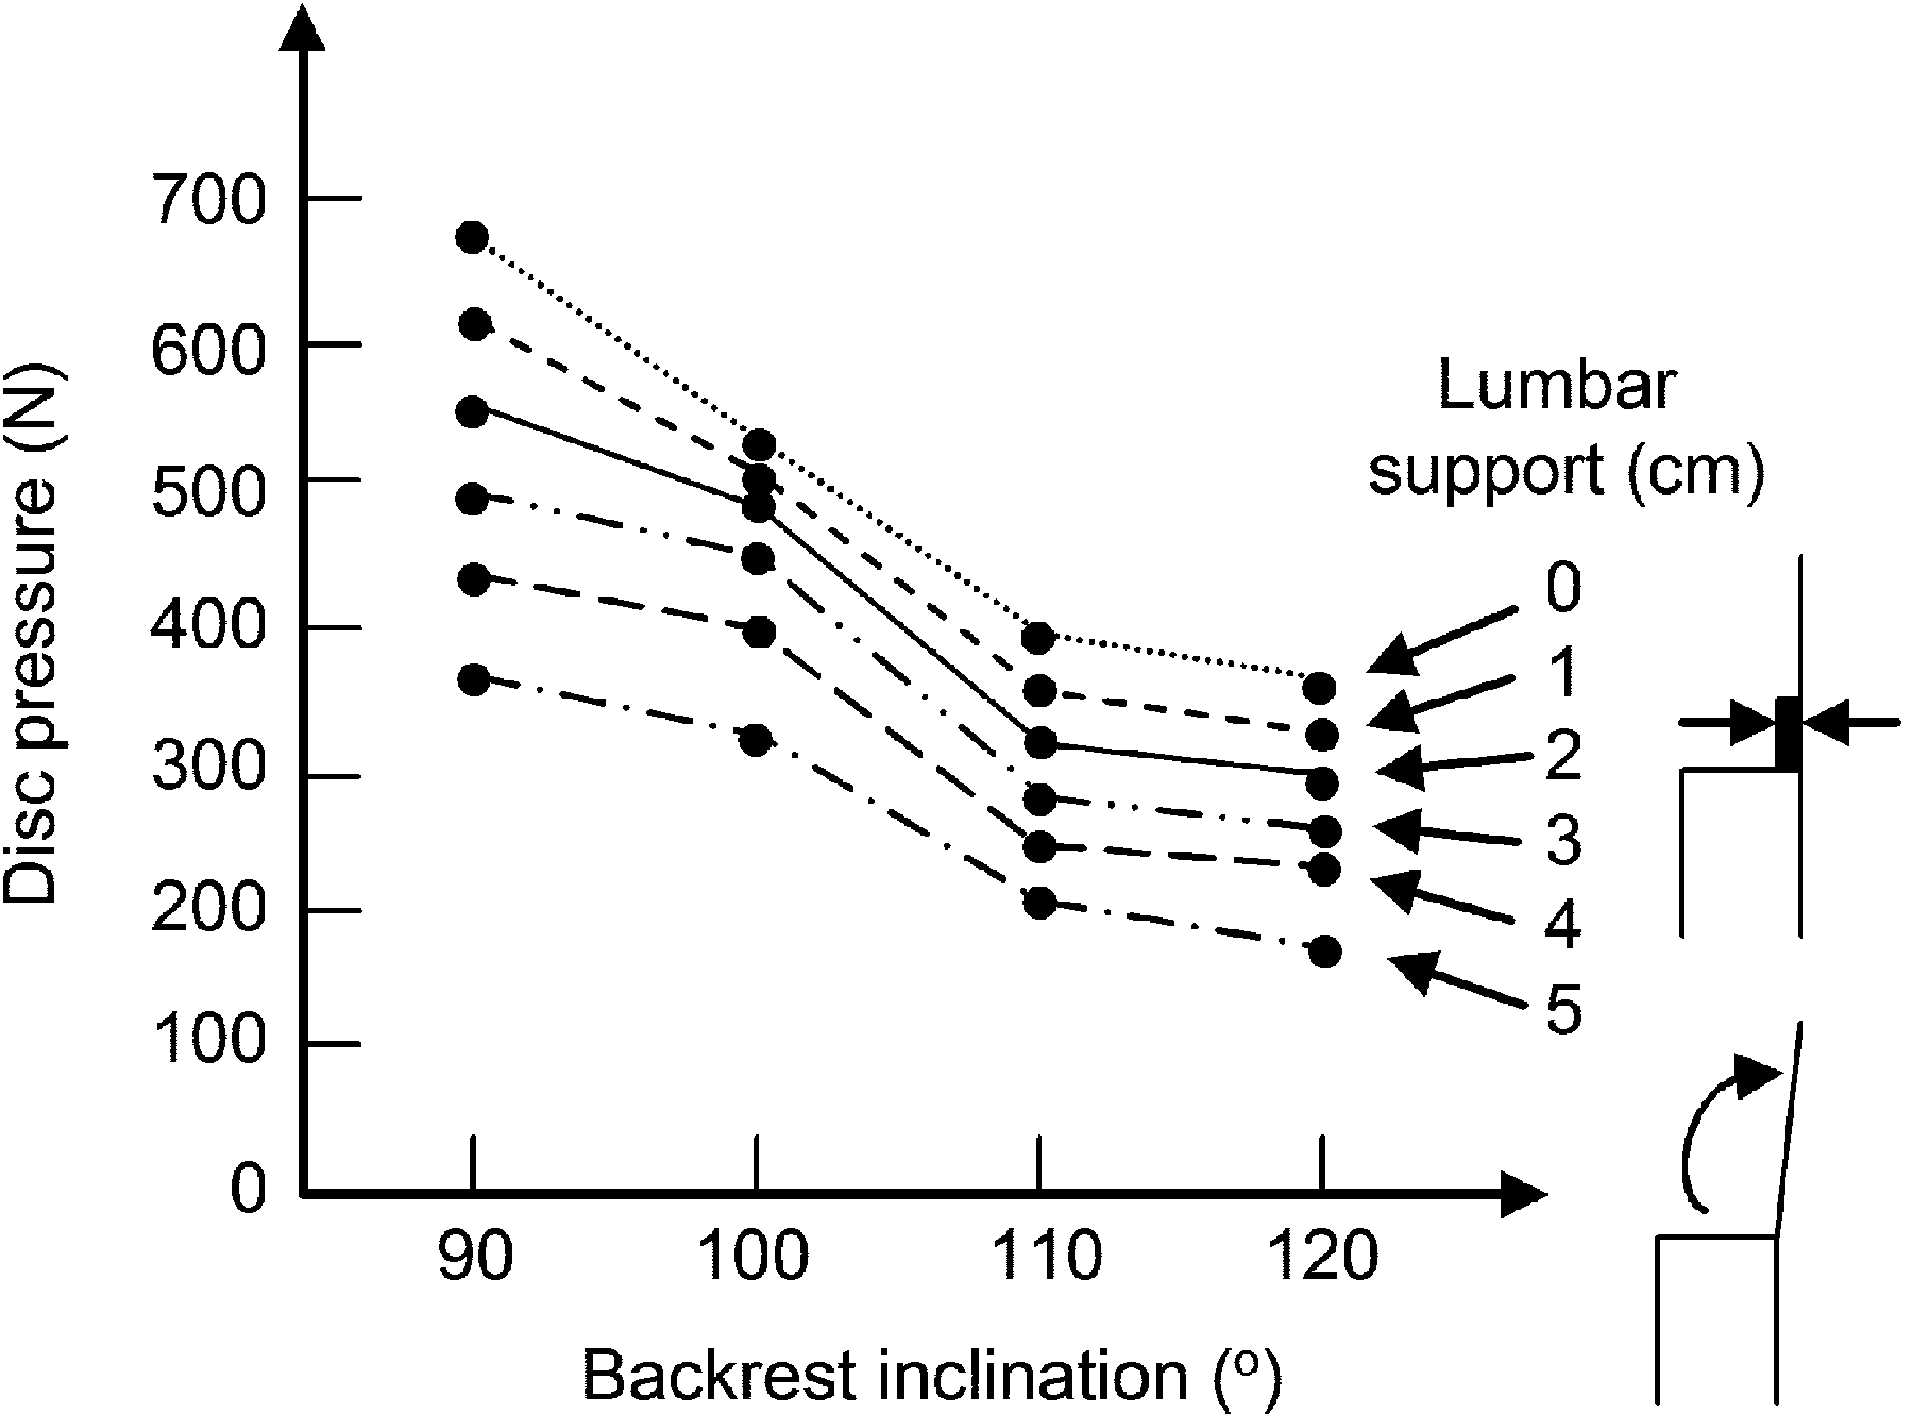
\includegraphics[width=0.75\textwidth]{245.png}
  \caption{La presión sobre el tercer disco lumbar disminuye con la inclinación del respaldo hacia atrás y con el soporte lumbar. Además, aumenta con el soporte en la región torácica, que no se muestra aquí. Las sillas con cierta inclinación hacia atrás y soporte lumbar proporcionan el apoyo necesario, mientras que aquellas con un respaldo plano y vertical o que se curvan hacia el cuerpo pueden causar una presión dolorosa. (Basado en \cite{2, 7}).}
  \label{fig:245}
\end{figure}

, pero cuando deba sentarse en sillas con respaldo plano, puede ser útil usar una toalla enrollada o una almohada en la parte inferior de la espalda para ayudar a mantener la curvatura.

Cuando duerma, mantenga una de estas dos posiciones: boca arriba con las rodillas dobladas y los pies encogidos (caderas y rodillas dobladas) o en posición fetal; nunca duerma boca abajo. (Una razón para esto es que en la posición decúbito supino con las piernas rectas, la porción vertebral del músculo psoas ejerce una carga sobre la columna lumbar, mientras que este músculo se relaja y esta carga disminuye cuando las caderas y las rodillas están dobladas y apoyadas \cite{25}). Solo duerma en camas que permitan que su espalda mantenga su curvatura natural; las camas no deben ser demasiado firmes ni demasiado blandas. En la Fig. 2.46 se muestran algunos ejercicios de hiperextensión que pueden fortalecer los músculos para ayudar a su espalda.

\begin{figure}[htbp]

  \centering
  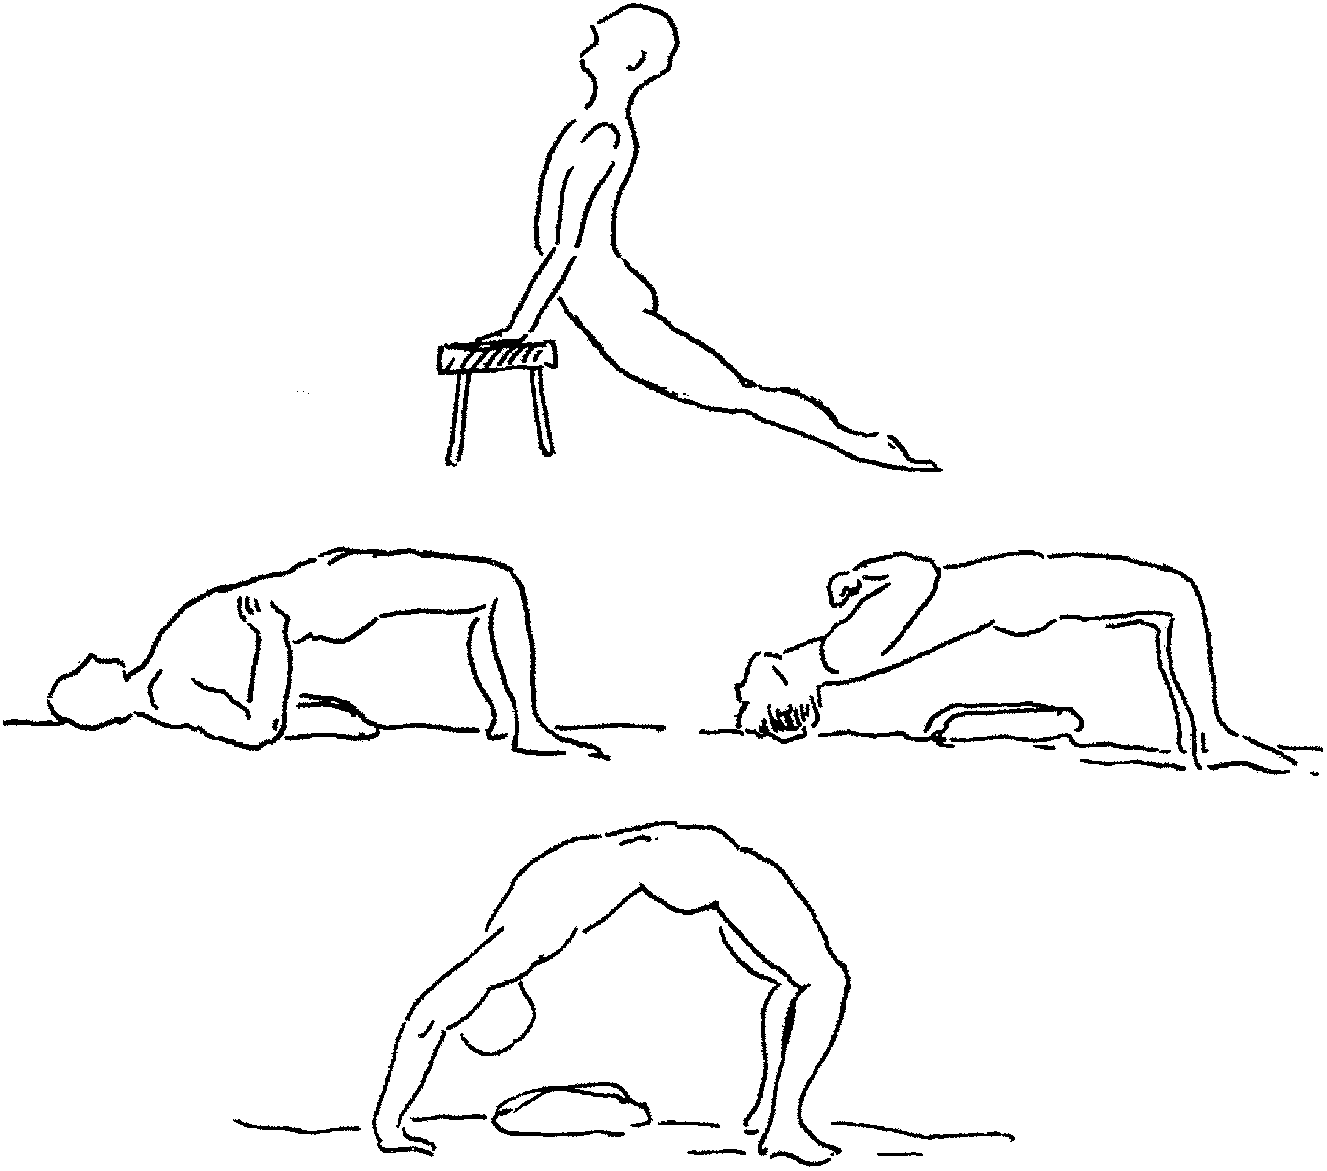
\includegraphics[width=0.75\textwidth]{246.png}
  \caption{Ejercicios de hiperextensión recomendados (en el Hospital Tientzin en China) para fortalecer la espalda de pacientes con lumbago (es decir, aquellos con dolor o molestia leve a severa en la parte baja de la espalda); cada uno se realiza manteniendo la espalda del paciente cóncava. También se recomiendan varios otros ejercicios para quienes tienen dolor lumbar. Si tiene dolor lumbar, consulte a su médico antes de intentar cualquiera de estos ejercicios. (De \cite{10}).}
  \label{fig:246}
\end{figure}

 (Adivine, ¿quién tiene un problema en la parte baja de la espalda?).

\subsection{Regla de las tres fuerzas}

Considere la combinación de pie y pierna inferior que se muestra en la Fig. 2.47a, la cual es un modelo para una persona que sube escaleras. Hay tres fuerzas que actúan sobre este sistema aislado. La fuerza normal $\vec{\mathbf{N}}$ actúa verticalmente en la parte anterior del pie y, para una subida lenta de escaleras, tiene una magnitud igual al peso corporal $W_b$. Esta fuerza normal intenta hacer rotar la pierna inferior en sentido horario al rededor de la rodilla. El tendón patelar transmite la fuerza del músculo cuádriceps del muslo $\vec{\mathbf{M}}$, como se muestra, e intenta contrarrestar esta rotación. La dirección de esta fuerza es a lo largo de este tendón y la dirección de este tendón es conocida. También hay una fuerza de reacción $\vec{\mathbf{R}}$ ejercida por los cóndilos femorales sobre la parte superior de la tibia, que actúa como se muestra en el punto $Q$. En este problema bidimensional, hay tres ecuaciones (dos para el equilibrio de fuerzas y una para el equilibrio de torques) y tres incógnitas: las magnitudes de $M$ y $R$, y la dirección de $\vec{\mathbf{R}}$. Como tal, este problema se puede resolver de la manera directa ilustrada anteriormente. Sin embargo, existe un procedimiento gráfico llamado la regla de las tres fuerzas que ofrece cierta comprensión adicional y, por supuesto, las mismas respuestas que el método directo. (Por simplicidad, estamos ignorando la masa de la pierna y del pie aquí).

\begin{SCfigure}[0.5][htbp]

  \centering
  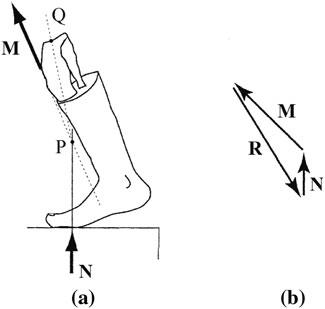
\includegraphics[width=0.55\textwidth]{247.png}
  \caption{\textbf{a} Ilustración de la regla de las tres fuerzas sobre la pierna inferior libre, con la fuerza de reacción $\vec{\mathbf{N}}$, la fuerza del tendón patelar $\vec{\mathbf{M}}$, el punto $P$ donde se cruzan las líneas de estos vectores extendidos y el punto $Q$ donde actúa la fuerza de la articulación sobre la tibia. \textbf{b} Diagrama vectorial de la regla de las tres fuerzas, donde $\vec{\mathbf{R}}$ es la fuerza de reacción de la articulación en $Q$. (De \cite{18}).}
  \label{fig:247}
\end{SCfigure}



Extendiendo los vectores $\vec{\mathbf{N}}$ y $\vec{\mathbf{M}}$, vemos que se intersectan en el punto $P$. Si elegimos el eje de rotación del torque perpendicular a este punto, vemos que estas dos fuerzas no contribuyen en nada al torque ya que sus vectores $\vec{\mathbf{r}}$ y $\vec{\mathbf{F}}$ son, respectivamente, antiparalelos y paralelos entre sí. Dado que en equilibrio estático (o en la situación cuasiestática aquí descrita) el torque neto es cero, el vector de la fuerza de reacción $\vec{\mathbf{R}}$ también debe pasar por $P$ cuando se extiende, por lo que $\vec{\mathbf{R}}$ es paralelo al segmento de línea $QP$. Debido a que las direcciones de $\vec{\mathbf{M}}$ y $\vec{\mathbf{R}}$ son ahora conocidas, podemos colocarlos en la cabeza y la cola de $\vec{\mathbf{N}}$, respectivamente, como se muestra en la Fig. 2.47b (siempre con la cabeza de un vector en la cola del otro, como al sumar vectores). Las longitudes de ambos vectores se determinan ahora alargándolos hasta que se toquen entre sí. Entonces, la suma de las fuerzas en las direcciones $x$ e $y$ es cero (debido al triángulo cerrado) y hemos obtenido toda la información necesaria.

Por cierto, las fuerzas de reacción en la rodilla son de $\sim 3\text{--}4 W_b$ durante la marcha \cite{24} y son mucho mayores al subir escaleras.

\subsection{Modelado multisegmento}

A menudo, varias partes del cuerpo son importantes al modelar el cuerpo, tanto en situaciones estáticas como en aquellas que involucran movimiento. Como ejemplo, la Fig. 2.48 muestra cómo un modelo anatómico de la pierna se puede modelar mediante tres segmentos que describen la pierna superior (muslo), la pierna inferior (pantorrilla) y el pie. Cada segmento se etiqueta por su masa ($m$), su centro de masa (punto) y su momento de inercia ($I$). En este ejemplo también hay tres articulaciones (bisagras o pasadores de rotación libre) entre la cadera y el muslo, entre el muslo y la pantorrilla (la rodilla) y entre la pantorrilla y el pie (el tobillo), cada una representada por un círculo abierto. Las fuerzas de los músculos y las fuerzas normales en las articulaciones y en otros lugares (como el suelo) se pueden añadir a este modelo de segmentos articulados, y se pueden analizar las fuerzas y los torques sobre todo el objeto, o bien se pueden analizar las fuerzas de cada segmento por sí mismo.

\begin{SCfigure}[0.5][htbp]

  \centering
  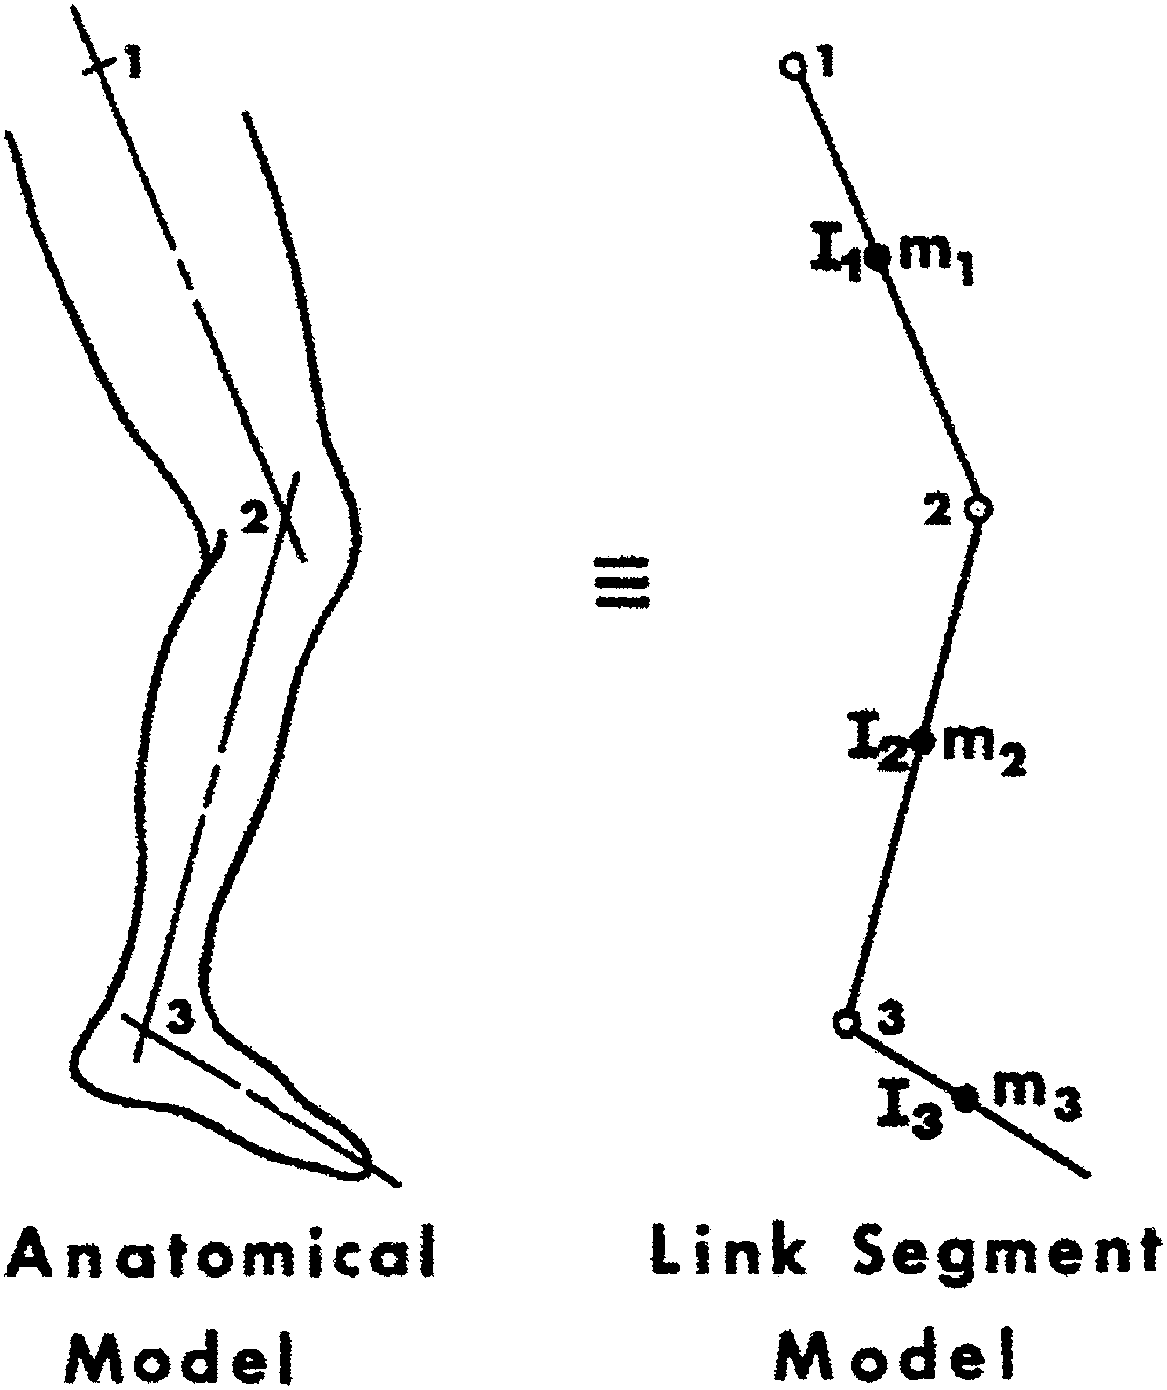
\includegraphics[width=0.5\textwidth]{248.png}
  \caption{Relación entre un modelo anatómico de la pierna y un modelo de segmentos articulados del muslo, la pantorrilla y el pie. (De \cite{39}. Reimpreso con permiso de Wiley).}
  \label{fig:248}
\end{SCfigure}

 (Esto es algo similar a examinar el cuerpo completo y luego la pierna por sí misma en el análisis anterior de la cadera).

Al analizar cada segmento de la Fig. 2.48 por separado, se llega a un diagrama de cuerpo libre para cada segmento, como en la Fig. 2.49. En este ejemplo se muestran las fuerzas de reacción en cada articulación del cuerpo ($\vec{\mathbf{R}}$), y en cada articulación particular las fuerzas son iguales en magnitud y opuestas en dirección debido a la Tercera Ley de Newton, como la fuerza $\vec{\mathbf{R}}_2$ que se muestra para la rodilla. Se podrían añadir las fuerzas debidas a cada músculo (o conjunto efectivo de músculos), que actúan con magnitudes iguales pero en direcciones opuestas en el origen y el punto de inserción (nuevamente, la Tercera Ley de Newton). (Esto se examina en el Problema 2.38). En el diagrama de cuerpo libre que se muestra en la Fig. 2.49, se muestra el torque total (que se llama momento $M$ en la figura) alrededor de cada articulación.

\begin{SCfigure}[0.5][htbp]

  \centering
  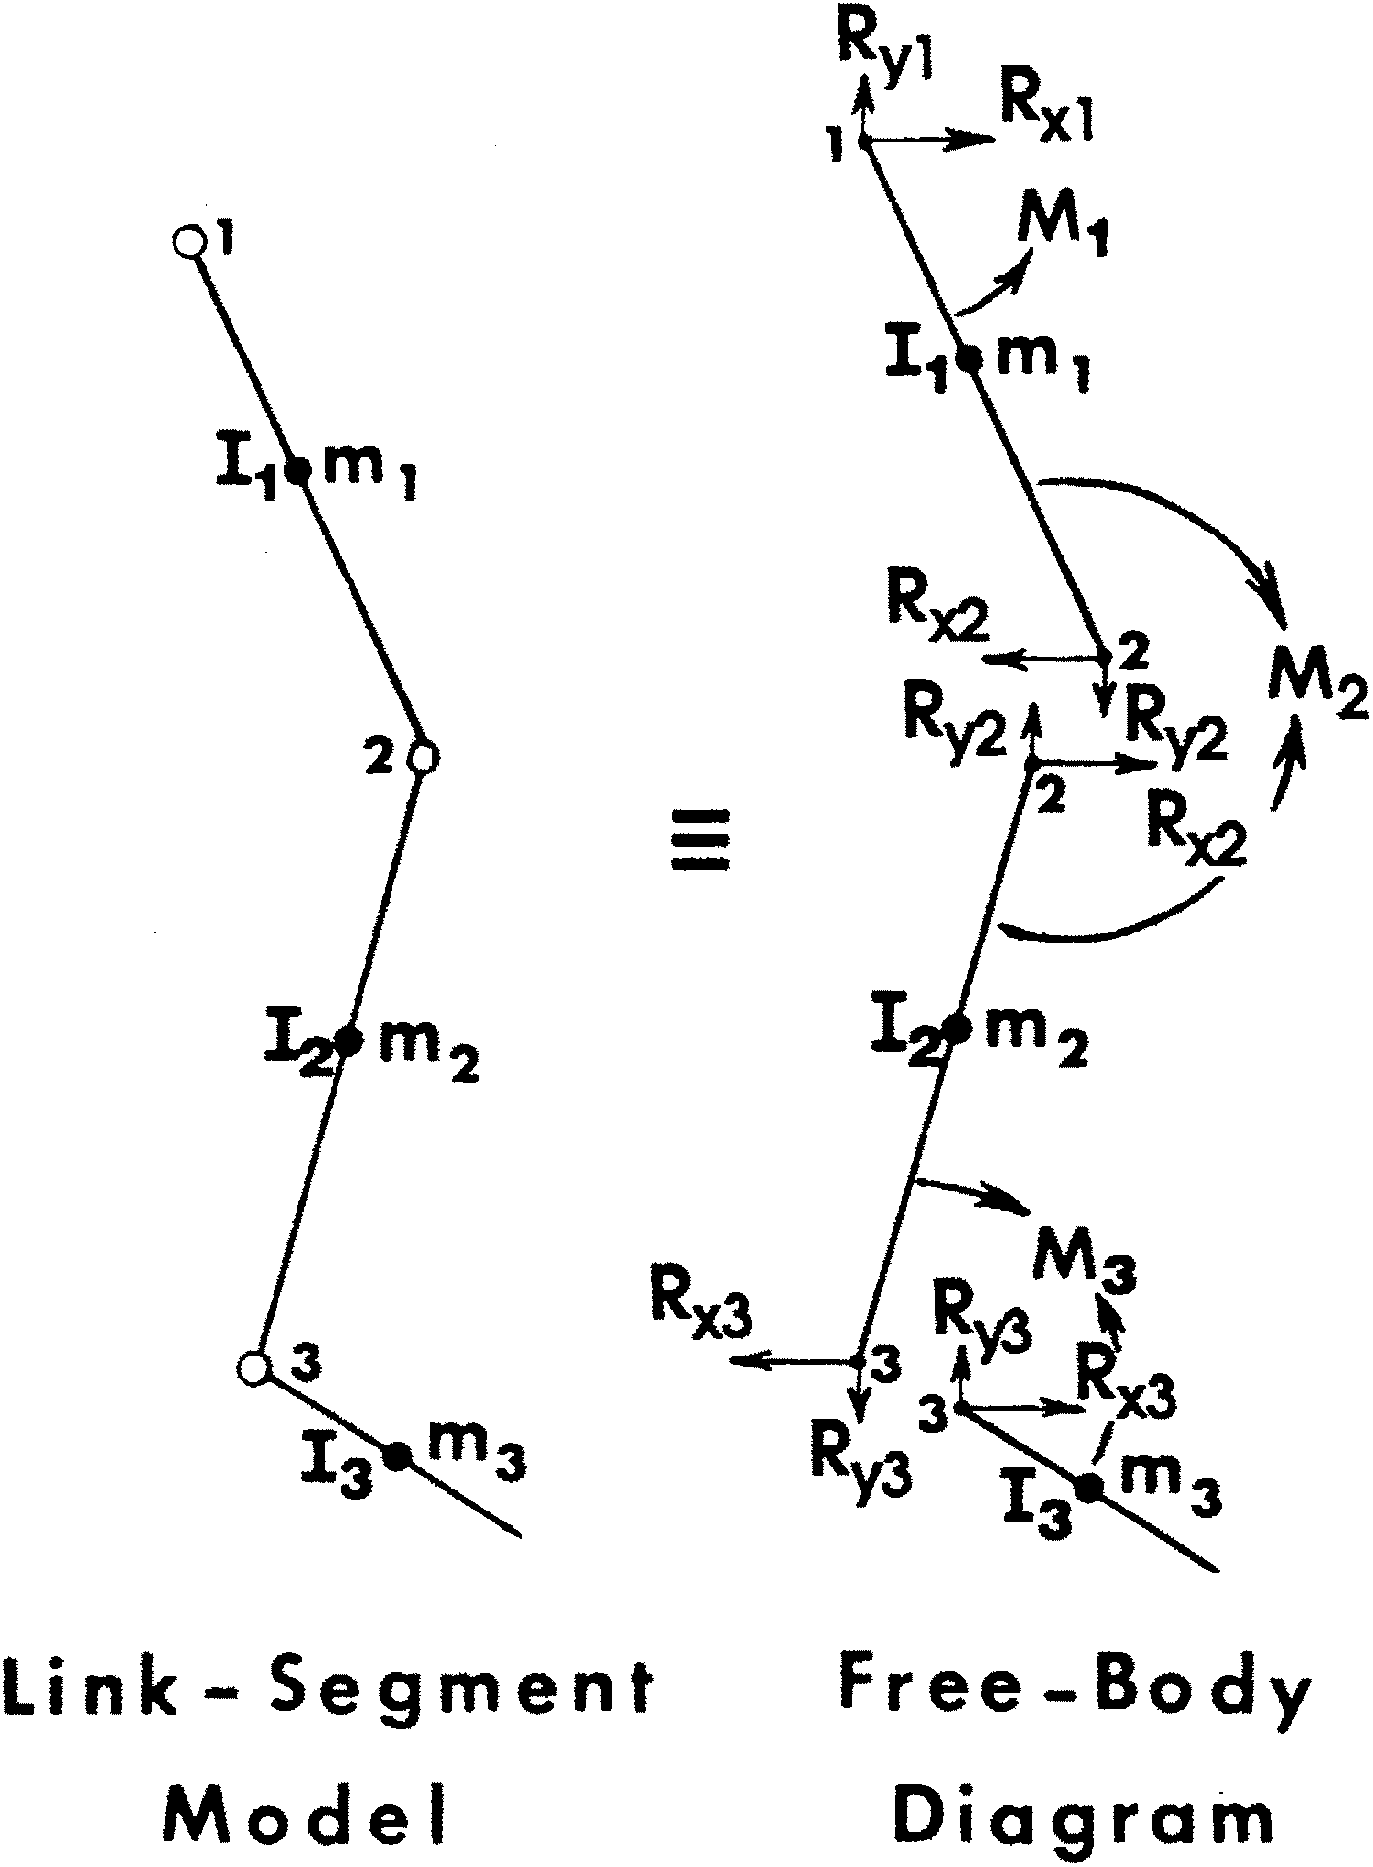
\includegraphics[width=0.5\textwidth]{249.png}
  \caption{Relación entre el modelo de segmentos articulados de la pierna y un diagrama de cuerpo libre con el muslo, la pantorrilla y el pie por separado. (De \cite{39}. Reimpreso con permiso de Wiley).}
  \label{fig:249}
\end{SCfigure}



En el Cap. 3 se presentan varios ejemplos del modelado multisegmento del movimiento.

\section{El sentido del tacto}

El cuerpo también «siente» la fuerza. Este es el sentido del tacto. Los sentidos somáticos incluyen el sentido del tacto por la piel (sensaciones cutáneas), el sentido de posición de las extremidades (propiocepción) y el sentido del movimiento de las extremidades (cinestesia). Existen sensores en la piel para la percepción táctil, la percepción de la temperatura y la percepción del dolor \cite{13}.

Existen cuatro tipos de receptores táctiles en la piel lampiña (sin pelo) (Fig. 2.50), cada uno sensible a esfuerzos y desplazamientos a diferentes frecuencias. Los receptores (o discos) de Merkel, ubicados cerca de la frontera entre la epidermis (la capa más externa de la piel) y la dermis (la capa subyacente), son más sensibles a las perturbaciones de presión que varían en el rango de $0,3\text{--}3\text{ Hz}$. Los otros receptores se encuentran a mayor profundidad dentro de la dermis. Los corpúsculos de Meissner detectan golpecitos ligeros, caracterizados por variaciones de $3\text{--}40\text{ Hz}$, y se perciben como un aleteo o vibración leve (\textit{flutter}). Los cilindros (o terminaciones) de Ruffini detectan vibraciones más rápidas, de $15\text{--}400\text{ Hz}$, como las causadas por el estiramiento de la piel o el movimiento de las articulaciones, y se perciben como un zumbido. Los corpúsculos de Pacini detectan un rango de vibraciones rápidas, de $10$ a $500\text{ Hz}$. El movimiento del vello también estimula estos receptores.

\begin{figure}[htbp]

  \centering
  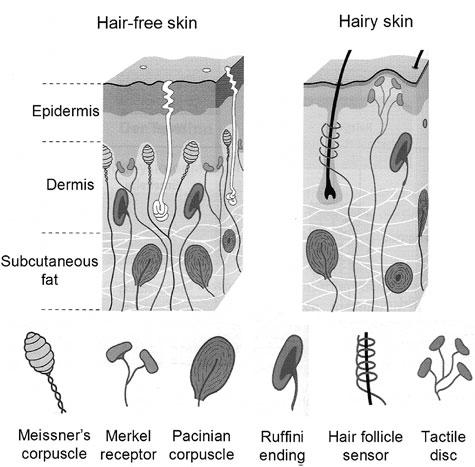
\includegraphics[width=0.55\textwidth]{250.png}
  \caption{Sección transversal de piel \textbf{a} lampiña y \textbf{b} vellosa, mostrando los sensores táctiles. (De \cite{31}).}
  \label{fig:250}
\end{figure}



La densidad espacial de los mecanorreceptores en la piel varía desde $25/\text{cm}^2$ en la punta de la lengua hasta $0,02/\text{cm}^2$ en la espalda \cite{4}. El movimiento del pelo en la piel vellosa contribuye al sentido del tacto, junto con la detección por parte de estos cuatro receptores. El mecanismo para convertir estos impulsos en señales eléctricas se analiza en el Cap. 12.

La piel también tiene dos tipos de receptores que detectan la temperatura. Los termorreceptores de fibras cálidas aumentan su tasa de disparo únicamente cuando hace más calor, y las fibras frías solo cuando hace más frío; no son sensibles a la estimulación mecánica. Las fibras cálidas responden de $30$ a $48^\circ\text{C}$, y mejor a unos $44^\circ\text{C}$, mientras que las fibras frías responden de $20$ a $45^\circ\text{C}$, y mejor a $30^\circ\text{C}$. Hay del orden de $5\text{--}10$ receptores térmicos por $\text{cm}^2$ en la mayor parte de la piel. Este sentido de la temperatura es importante en el esfuerzo del cuerpo por controlar la temperatura (Cap. 13).

Los nociceptores en la piel detectan la presión excesiva, la temperatura extrema y los productos químicos corrosivos, cada uno de los cuales puede dañar la piel. Algunos receptores del dolor transmiten señales muy rápidamente al cerebro, a través de axones mielinizados en neuronas con velocidades de conducción de hasta $30\text{ m/s}$ (ver Cap. 12). Algunos receptores de dolor indican dolor persistente y tienen señales que se transmiten en axones no mielinizados muy lentos con velocidades de $2\text{ m/s}$ y menores.

Como se caracteriza por la Ley de Stevens ((1.6), Tabla 1.15), la variación del estímulo percibido es ligeramente sublineal con la fuerza del estímulo para la vibración, algo superlineal para la sensación de presión en la palma y la pesadez de los objetos levantados, lineal para el frío y superlineal para el calor.

Un problema en el Cap. 7 (Problema 7.14, Fig. 7.25) aborda cómo usar el sentido del tacto para estimar la presión interna en un vaso elástico. Este es un ejemplo de palpación, que es el uso de las manos del médico para examinar partes del cuerpo durante un examen médico. (Un médico también da golpecitos en el cuerpo en el diagnóstico conocido como percusión. A tercer diagnóstico físico es escuchar los sonidos que emanan del cuerpo, lo que se denomina auscultación; se analiza en el Cap. 10).

\section{Desviación hacia las unidades de fuerza y presión}

\subsection{Fuerza}

Debemos tener claras las unidades correctas de fuerza, como se muestra en la Tabla 2.5. En el sistema inglés (o FPS) son las libras (lb). En el sistema métrico MKS-SI son los newtons (N) y en los sistemas CGS son las dinas. La mayor parte del trabajo técnico se realiza en MKS-SI; sin embargo, gran parte del trabajo médico se realiza utilizando el sistema inglés (en los EE. UU.). Normalmente utilizaremos lb o N, usando lb cuando nos refiramos a los pesos corporales. (Ver también el Apéndice A).

\begin{table}[htbp]
\centering
\caption{Unidades de fuerza.}
\label{tab:25}
\begin{tabular}{l}
\toprule
$1\text{ N} = 1\text{ kg}\cdot\text{m/s}^2$ \\
$1\text{ N} = 10^5\text{ dinas}$ \\
$1\text{ N} = 0,225\text{ lb } (\sim 2/9\text{ lb})$ \\
$1\text{ lb} = 4,45\text{ N}$ \\
\bottomrule
\end{tabular}
\end{table}

Un kilogramo ($\text{kg}$) es una masa ($m$) que al nivel del mar (en el planeta Tierra) tiene un peso de $9,8\text{ N}$ (o $2,2\text{ lb}$). Esto es una consecuencia de la aceleración gravitacional en la Tierra y de la Segunda Ley del movimiento de Newton
\begin{equation}
F = mg,
\label{eq:2.47}
\end{equation}
donde $g = 9,8\text{ m/s}^2$. «$g$» es la aceleración de cualquier objeto en caída libre debido a la gravedad. En unidades CGS, una masa de $1\text{ g}$ tiene un peso de $980,7\text{ dinas}$ porque $g = 980,7\text{ cm/s}^2$. En el sistema inglés, $g = 32,2\text{ ft/s}^2$. La unidad de masa en el sistema inglés es el slug; rara vez se utiliza en los EE. UU. Un slug tiene un peso de $32,2\text{ lb}$.

A veces, en la literatura de biomecánica se proporciona la masa de carga, y es posible que se haga referencia errónea a la unidad «$\text{kg}$» como una fuerza. Lo que realmente se quiere decir es el peso de un objeto con una masa de $1\text{ kg}$. Para reducir la confusión, esto debería expresarse como $1\text{ kg}$ (fuerza). Mejor aún, cuando se vea $1\text{ kg}$ (fuerza), debería reemplazarse por $9,8\text{ N}$ ($\sim 10\text{ N}$).

\subsection{Presión}

Más adelante nos encontraremos con el concepto de presión. La presión ($P$) es simplemente una fuerza por unidad de área. (De manera más general, una fuerza por unidad de área es un esfuerzo (Tabla 2.6). La presión, o más precisamente la presión hidrostática, es un esfuerzo que es el mismo en todas las direcciones). Las unidades de presión (o esfuerzo $\sigma$) son las unidades de fuerza divididas por las unidades de área.

\begin{table}[htbp]
\centering
\caption{Unidades de presión.}
\label{tab:26}
\small
\begin{tabular}{l}
\toprule
$1\text{ N/m}^2 = 1\text{ Pa} = 9,87 \times 10^{-6}\text{ atm.} = 0,0075\text{ mmHg} = 0,102\text{ mmH}_2\text{O}$ \\
$1\text{ N/mm}^2 = 10^6\text{ N/m}^2 = 10^6\text{ Pa} = 1\text{ MPa} = 145\text{ psi} = 9,87\text{ atm.} \simeq 10\text{ atm.}$ \\
$1\text{ psi} = 0,0069\text{ N/mm}^2 = 6.894,8\text{ N/m}^2\text{ (o Pa)} = 1/14,7\text{ atm.} = 0,068\text{ atm.}$ \\
$1\text{ bar} = 10^5\text{ N/m}^2\text{ (o Pa)} = 0,1\text{ N/mm}^2 \simeq 1\text{ atm.}$ \\
$1\text{ atm.} = 1,013 \times 10^5\text{ Pa} = 1,013\text{ bar} = 0,103\text{ N/mm}^2\text{ (o MPa)} = 14,7\text{ psi}$ \\
$\quad = 760\text{ mmHg} = 29,9\text{ pulgadas de Hg} = 1.033\text{ cmH}_2\text{O} = 407\text{ pulgadas de H}_2\text{O}$ \\
$1\text{ mmHg} = 0,00132\text{ atm.} = 133\text{ N/m}^2 = 13,6\text{ mmH}_2\text{O}$ \\
$1\text{ mmH}_2\text{O} = 0,1\text{ cmH}_2\text{O} = 9,68 \times 10^{-5}\text{ atm.} = 9,81\text{ N/m}^2 = 0,0735\text{ mmHg}$ \\
$1\text{ kg (fuerza)/cm}^2 = 9,8\text{ N/cm}^2$ \\
\bottomrule
\end{tabular}
\end{table}

A menudo utilizaremos $\text{MPa}$ ($=\text{ N/mm}^2$), pero ocasionalmente usaremos otras unidades, como $\text{mmHg}$ al discutir la presión arterial.

Debido a que el trabajo (o energía) es fuerza $\times$ distancia, las unidades de presión son las mismas que las de energía/volumen. (Ver también el Apéndice A).

La unidad estándar MKS-SI de presión es el pascal ($\text{Pa}$), con $1\text{ Pa} = 1\text{ N/m}^2$. A menudo encontraremos que los números que hallaremos son más simples en unidades de $\text{N/mm}^2$, que son las mismas que las unidades de $\text{MPa}$. Las unidades comunes en el sistema inglés son las libras por pulgada cuadrada ($\text{psi}$).

Estas unidades son independientes del planeta en el que nos encontremos. Algunas unidades comunes de presión son específicas de la Tierra (al nivel del mar, a una temperatura de $0^\circ\text{C}$). Una columna de un líquido de densidad de masa $\rho$ y altura $h$ ejerce una presión
\begin{equation}
P = \rho g h.
\label{eq:2.48}
\end{equation}

Esto es lo mismo que (2.47), después de dividir ambos lados por el área de la columna $A$, porque $P = F/A$ y $m = \rho \times\text{ volumen} = \rho A h$. Al nivel del mar en la Tierra ($0^\circ\text{C}$), la presión del aire es $1\text{ atmósfera}$ ($1\text{ atm.}$), que es la presión ejercida por la columna de aire sobre ella. La misma presión es ejercida por $760\text{ mm}$ de $\text{Hg}$ (mercurio) o $1.033\text{ cm}$ de agua. Las unidades de $\text{mmHg}$ y $\text{cmH}_2\text{O}$ (o pulgadas de $\text{H}_2\text{O}$) se utilizan muy comúnmente a pesar de que en realidad se refieren a $h$ en (2.48) y no a la presión. (En un cálculo, deben multiplicarse por $\rho_{\text{Hg}} = 13,6\text{ g/cm}^3$ o $\rho_{\text{H}_2\text{O}} = 1,0\text{ g/cm}^3$ y luego por $g$. Tenga en cuenta que $\rho_{\text{sangre}} = 1,06\text{ g/cm}^3$). En los EE. UU., la presión del aire se expresa comúnmente en los informes meteorológicos en unidades de pulgadas de $\text{Hg}$, como en «la presión del aire es $29,8\text{ in}$ y está bajando». La presión arterial se informa comúnmente en $\text{mmHg}$, como en 120/80, lo que significa que las presiones sistólica y diastólica son, respectivamente, $120\text{ mmHg}$ y $80\text{ mmHg}$. Las presiones de aire en el cuerpo, como en los pulmones, a veces se expresan en términos de $\text{cm}$ o pulgadas de agua, porque es una unidad más pequeña y mucho más conveniente. La presión a menudo se refiere a la presión atmosférica, por lo que una presión arterial de $120\text{ mmHg}$ realmente significa una presión absoluta que está $120\text{ mmHg}$ por encima de la presión atmosférica (con $1\text{ atm.} = 760\text{ mmHg}$), y como tal se denomina presión manométrica.

Es una coincidencia sorprendente que la unidad de presión atmosférica basada en la Tierra ($1\text{ atm.}$) esté dentro del 1\% de la unidad basada en MKS-SI, independiente de la Tierra, de un «bar» ($1\text{ bar} = 10^5\text{ N/m}^2$ (o $\text{Pa}$)), con $1\text{ atm.} = 1,013\text{ bar}$.

\section{Resumen}

El equilibrio de fuerzas y torques a menudo se puede analizar en términos de palancas, como en el caso del antebrazo. El equilibrio de una parte del cuerpo se puede analizar examinando las fuerzas debidas a la gravedad, los músculos y las fuerzas de reacción en todo el cuerpo y en esa parte del cuerpo por separado. Las fuerzas musculares y las fuerzas de reacción internas pueden superar el peso corporal, como se vio al analizar las fuerzas en la cadera y la parte baja de la espalda, y esto puede tener consecuencias graves.

\section*{Problemas}

\subsection*{Estática del brazo y palancas}

\begin{enumerate}
\item[2.1] Una persona sostiene un peso con el brazo extendido horizontalmente, utilizando sus músculos deltoides para equilibrar el peso alrededor de la articulación del hombro. ¿Qué tipo de palanca es esta? Dibuje y etiquete esta palanca.

\item[2.2] Una persona se sostiene a sí misma en posición de lagartija (flexión de brazos). Considere uno de los brazos de la persona, con el punto de pivote en la mano apoyada en el suelo. ¿Están involucrados el bíceps braquial o el tríceps braquial? ¿Qué tipo de palanca es esta? Dibuje y etiquete esta palanca.

\item[2.3] Para cada uno de los siguientes casos, identifique el tipo de palanca y muestre en un esquema las ubicaciones de la fuerza aplicada, el punto de apoyo (fulcro) y la carga aplicada:

(a) cortar con un par de tijeras

(b) levantar una carretilla

(c) recoger algo con un par de pinzas.

\item[2.4] Analice el equilibrio de fuerzas en las direcciones $x$ e $y$ y el equilibrio de torques en la dirección $z$ para el antebrazo, con un brazo superior vertical y un antebrazo horizontal (longitud de $35\text{ cm}$) (Fig. 2.9). Al igual que en el Caso 1 del texto, ignore el peso del antebrazo y otros músculos. Ahora se incluye explícitamente el efecto de la fuerza de reacción $\vec{\mathbf{N}}$ en la articulación (con componentes $N_x$ y $N_y$) (dado que no aporta ningún torque, no tuvo que incluirse en el análisis del Caso 1 anterior) y asuma que los bíceps están unidos a $4\text{ cm}$ del pivote a un ángulo $\theta$ con respecto al antebrazo. Con $\theta = 75^\circ$, halle la fuerza muscular $M$ y la magnitud de la fuerza de reacción en términos del peso $W$ y el ángulo de esta fuerza de reacción con respecto al eje $x$ (horizontal).

\subsection*{Estática de la cadera y la pierna}

\item[2.5] Utilizando la Fig. 1.15, ¿qué puede decir sobre la altura de la persona cuya pierna se representa en la Fig. 2.17?

\item[2.6] Muestre cómo las dimensiones dadas en la Fig. 2.16 cambian a las de la Fig. 2.20 cuando la persona sostiene un bastón.

\item[2.7] Al examinar las fuerzas de la cadera durante el equilibrio de un hombre parado sobre un pie, asumimos que el ángulo efectivo de los músculos abductores de la cadera con respecto al eje $x$ era el mismo, $70^\circ$, con o sin bastón. ¿Afectaría significativamente el uso de valores más realistas (y diferentes) de este ángulo, con o sin bastón, a las conclusiones sobre el efecto de usar un bastón?

\item[2.8] Un hombre de $200\text{ lb}$ se para sobre su pie derecho mientras lleva una bolsa de $100\text{ lb}$ en su mano izquierda. El centro de masa de la bolsa está a $12\text{ in}$ de su centro de masa (ver Fig. 2.51).

\begin{SCfigure}[0.5][htbp]

  \centering
  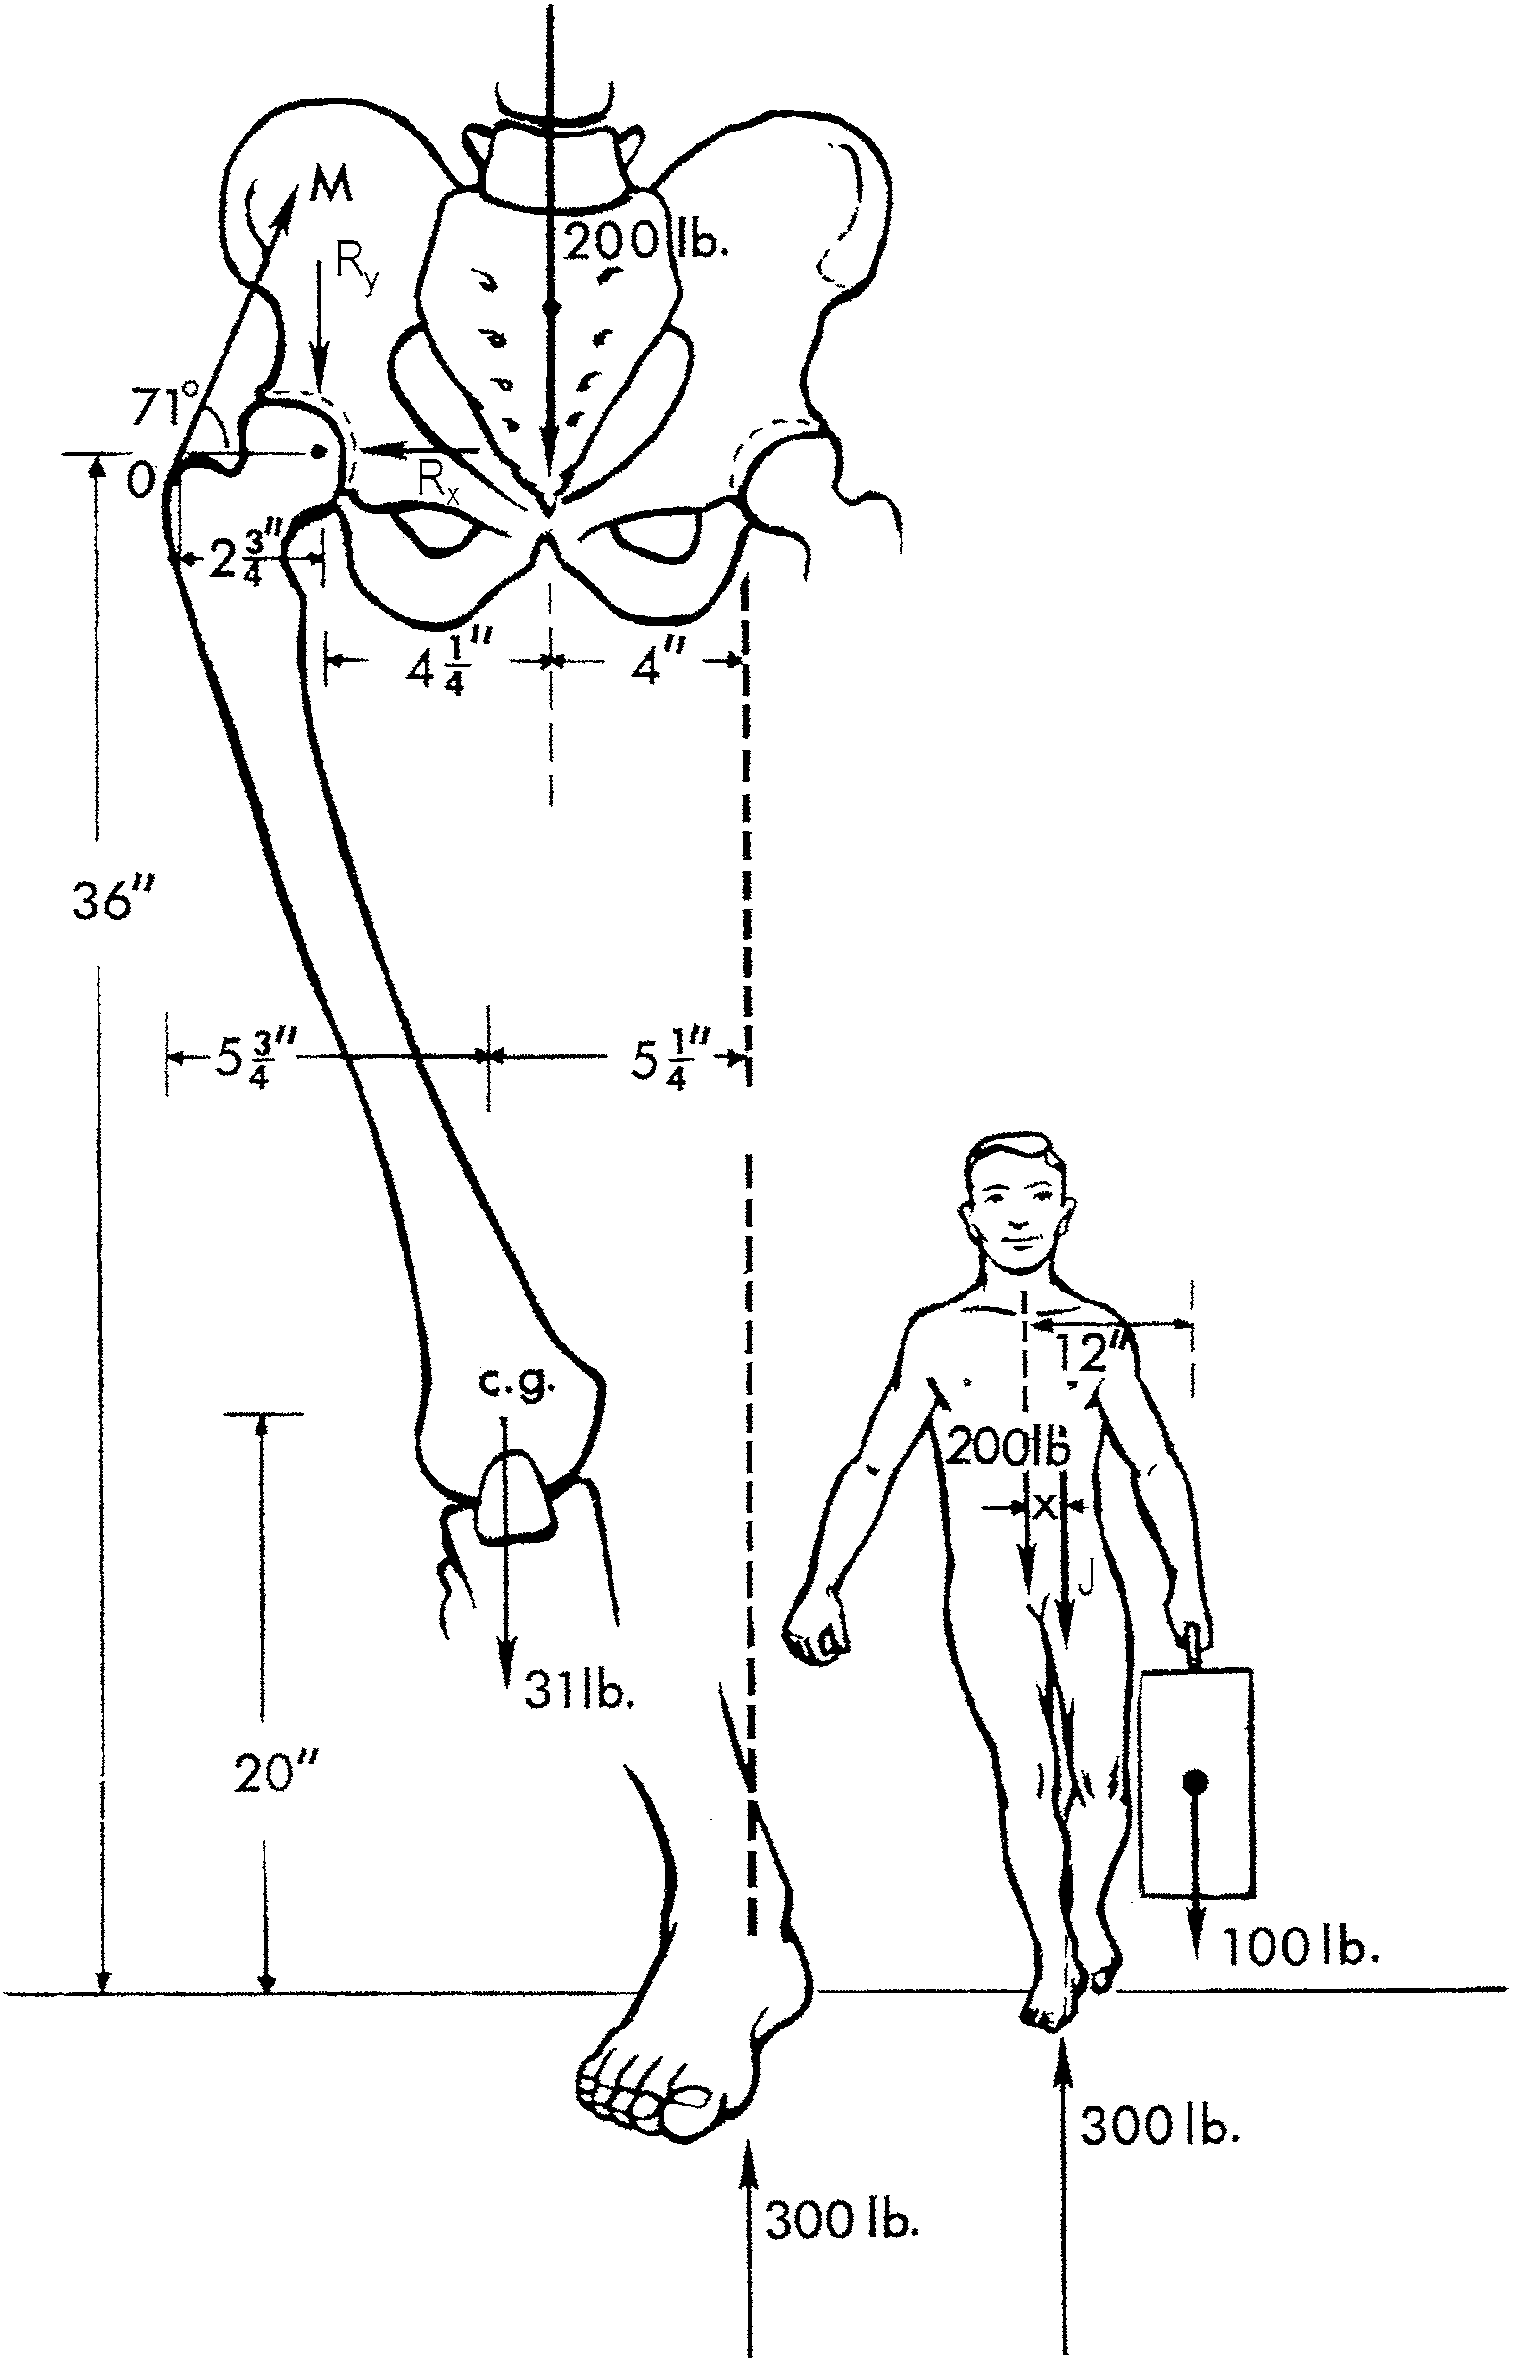
\includegraphics[width=0.5\textwidth]{251.png}
  \caption{Fuerzas sobre la cadera y la cabeza femoral al estar parado sobre una pierna y levantar un peso con la mano opuesta. (Reimpreso de \cite{15}. Usado con permiso de Elsevier). Para el Problema 2.8.}
  \label{fig:251}
\end{SCfigure}



(a) Demuestre que la colocación del pie (como se muestra) no genera un torque neto en el cuerpo.

(b) Halle la fuerza (su magnitud y dirección) sobre la cabeza del fémur de apoyo y la fuerza en el músculo abductor de la cadera examinando la pierna derecha.

(c) Compare sus respuestas en las partes (a) y (b) con lo que se encontró para el hombre que no sostiene masa alguna, con y sin bastón (para $W_b = 880\text{ N} = 200\text{ lb}$). ¿Son las fuerzas aquí mayores que para un hombre de ($200\text{ lb} + 100\text{ lb} =$) $300\text{ lb}$ (sin bastón)? ¿Por qué? (El ángulo muscular y la masa de la pierna son solo insignificantemente diferentes para el problema presentado aquí y los analizados anteriormente).

\item[2.9] Vuelva a dibujar la Fig. 2.51, cambiando todas las distancias y fuerzas a unidades métricas, y luego resuelva el Problema 2.8.

\item[2.10] Calcule la fuerza sobre los músculos abductores de la cadera para una persona parada simétricamente sobre dos pies, como una función de la separación de los pies. ¿Para qué posición es esta fuerza cero?

\item[2.11] En la posición de arabesca, una gimnasta inicialmente erguida patea una pierna hacia atrás y hacia arriba mientras la mantiene recta (masa $m_{\text{pierna}}$), empuja su torso y cabeza hacia adelante (masa $m_{\text{torso+cabeza}}$) y propulsa sus brazos hacia atrás y hacia arriba mientras los mantiene rectos (cada uno de masa $m_{\text{brazo}}$). Estos forman, respectivamente, ángulos agudos $\theta_{\text{pierna}}$, $\theta_{\text{torso+cabeza}}$ y $\theta_{\text{brazos}}$ con la horizontal. Los centros de masa de la pierna extendida y de la pierna de apoyo vertical están a una distancia $x_{\text{pierna extendida}}$ y $x_{\text{pierna de apoyo}}$ detrás de la vertical desde el centro de masa (en el plano sagital medio), y el de la parte superior de su cuerpo (combinación de torso/cabeza/brazos) está a una distancia $x_{\text{cuerpo superior}}$ por delante de esta vertical (por lo que todas estas distancias se definen como positivas). Al lograr esta posición de arabesca, su centro de masa desciende verticalmente desde la altura $y_{\text{antes}}$ a $y_{\text{después}}$.

(a) Dibuje un diagrama que muestre a la gimnasta antes y durante esta maniobra.

(b) Halle la condición de equilibrio en términos de estas masas y distancias. (Sugerencia: Analice los torques alrededor de su centro de masa en la posición de arabesca. Puede ignorar la contribución de sus brazos. ¿Por qué? Es posible que no necesite toda la información presentada).

(c) Asuma que la gimnasta mide $1,49\text{ m}$ ($4\text{ ft } 11\text{ in}$) de estatura y tiene una masa de $38\text{ kg}$ (peso de $84\text{ lb}$), y su pierna libre y sus brazos forman un ángulo de $30^\circ$ con la horizontal. ¿Qué ángulo forma la parte superior de su cuerpo con la horizontal? (Asuma las relaciones antropométricas para un humano estándar).

\item[2.12] Repita el Problema 2.11c si la pierna libre de la gimnasta está horizontal y sus brazos están verticales. (Esta es la posición de porrista).

\item[2.13] (a) Calcule el torque de la clavadista de masa $m_b$ alrededor del eje que pasa por sus dedos de los pies (normal a un plano sagital) cuando está en un trampolín e inclinada hacia adelante a punto de zambullirse, de modo que el eje vertical que pasa por su centro de masa está a una distancia $x$ por delante de sus dedos.

(b) Ahora suponga que la clavadista tiene una altura $H$ y que su cuerpo está proporcionado de acuerdo con los datos dados en el Cap. 1. Calcule el torque en términos de $H$, con su cuerpo recto y los brazos estirados paralelos a su torso. Asuma que su cuerpo puede estar recto (y por lo tanto todo en su cuerpo puede aproximarse como si estuviera en un plano) e ignore el cambio de posición debido a que está sobre sus dedos de los pies.

(c) Repita esto si sus brazos están en cambio a lo largo de sus costados. ¿Cómo difiere este torque del de la parte (b)?

\item[2.14] El dispositivo de tracción Russell dividida se utiliza para estabilizar la pierna, como se representa en la Fig. 2.52, junto con el diagrama de fuerzas relevante \cite{28}.

\begin{SCfigure}[0.5][htbp]

  \centering
  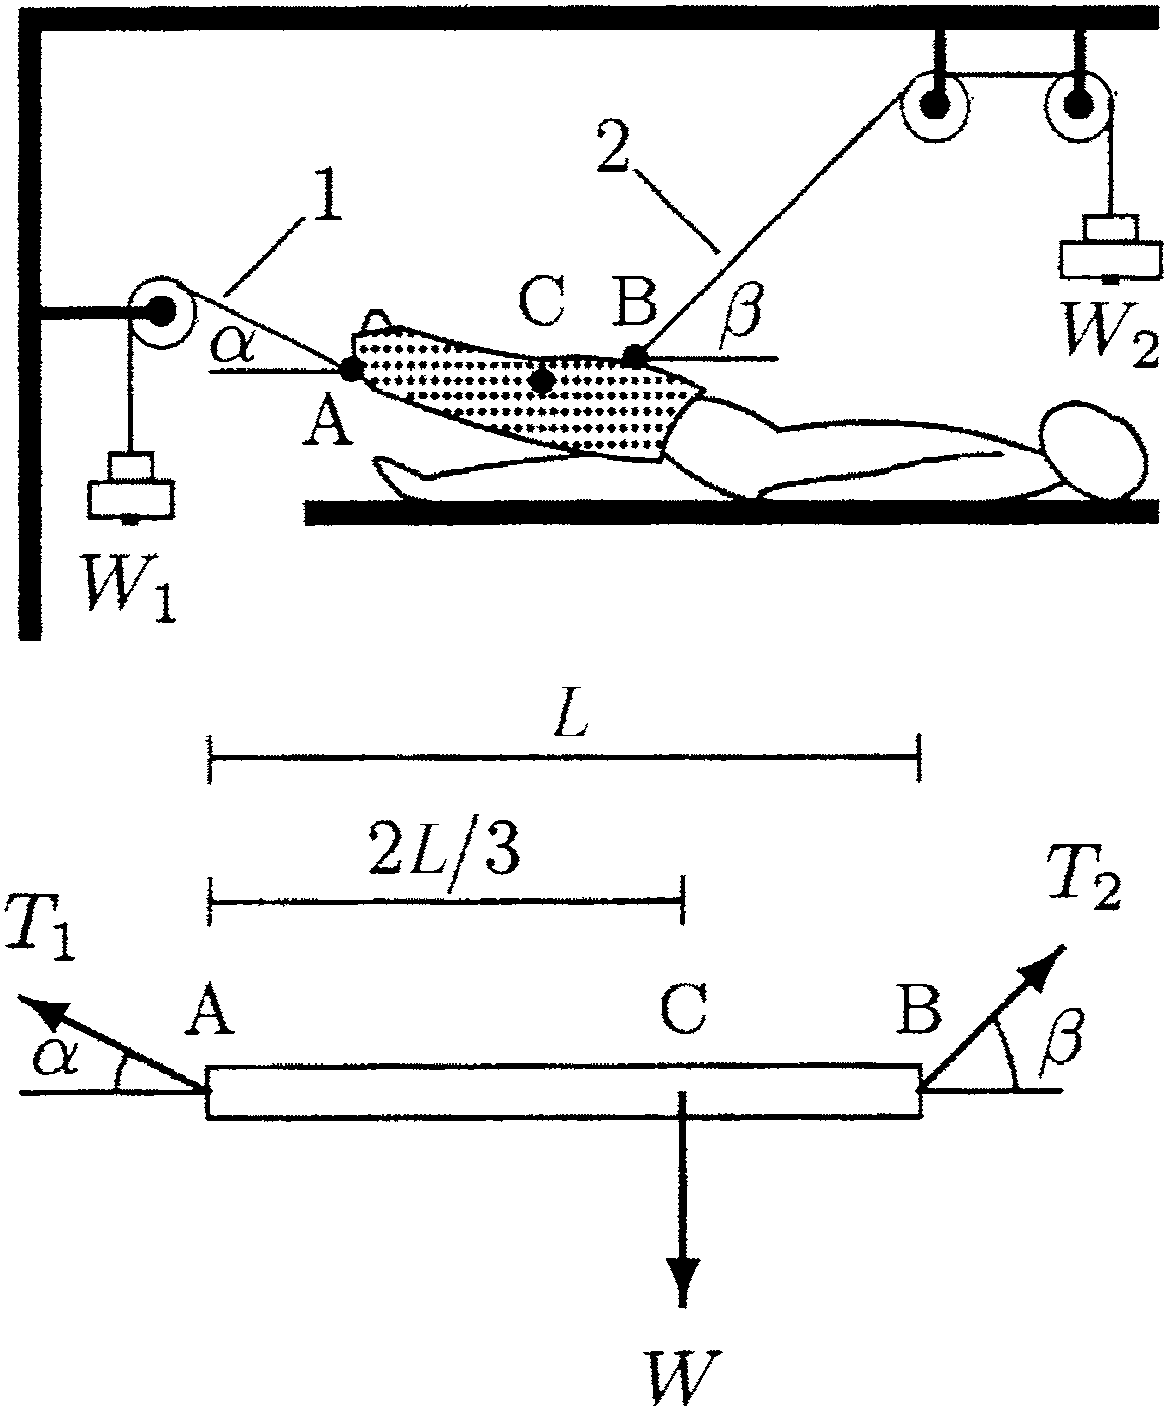
\includegraphics[width=0.55\textwidth]{252.png}
  \caption{El dispositivo de tracción Russell dividida (\textit{split Russel}). (De \cite{28}). Para el Problema 2.14.}
  \label{fig:252}
\end{SCfigure}

 La pierna se estabiliza mediante dos pesos, $W_1$ y $W_2$, unidos a la pierna por dos cables. La pierna y el yeso tienen un peso combinado de $W_1 = 300\text{ N}$ y un centro de masa a dos tercios de la distancia desde la izquierda, como se muestra. El cable para $W_2$ forma un ángulo $\beta = 45^\circ$ con la horizontal. Para el equilibrio, halle la tensión en los cables $T_1$ y $T_2$ y el ángulo $\alpha$ que el cable para $W_1$ forma con la horizontal.

\subsection*{Estática del hombro, la rodilla, el tobillo y la mandíbula}

\item[2.15] La porción clavicular del músculo pectoral mayor ejerce una fuerza de $224\text{ N}$ a un ángulo de $0,55\text{ rad}$ por encima de la horizontal, y la porción esternal del mismo ejerce una fuerza de $251\text{ N}$ a un ángulo de $0,35\text{ rad}$ por debajo de la horizontal, ambas en el plano que contiene al húmero vertical. Halle la magnitud resultante de la fuerza total y su dirección, y esquematice los tres vectores de fuerza en relación con el húmero. (De \cite{9}).

\item[2.16] Usted es capaz de mantener su brazo en una posición extendida debido al músculo deltoides (Fig. 2.53). El diagrama de fuerzas para esto se muestra en la Fig. 2.54.

\begin{SCfigure}[0.5][htbp]

  \centering
  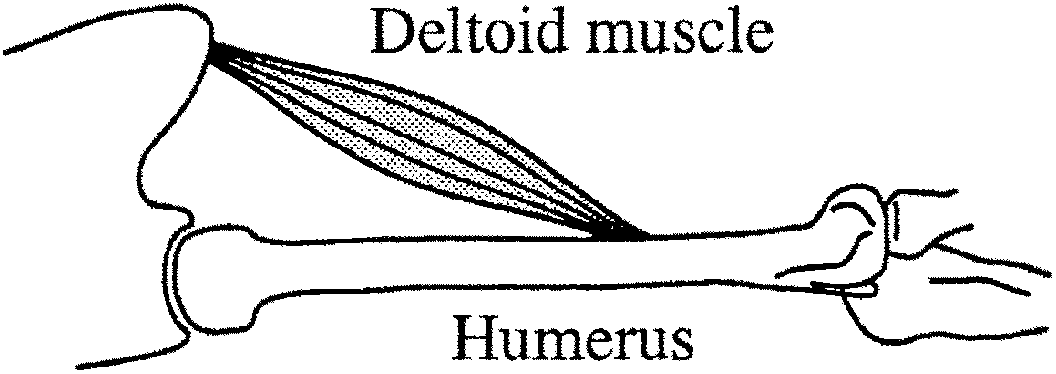
\includegraphics[width=0.55\textwidth]{253.png}
  \caption{Músculo deltoides durante el levantamiento con un brazo extendido. (De \cite{3}). Para el Problema 2.16.}
  \label{fig:253}
\end{SCfigure}

\begin{SCfigure}[0.5][htbp]

  \centering
  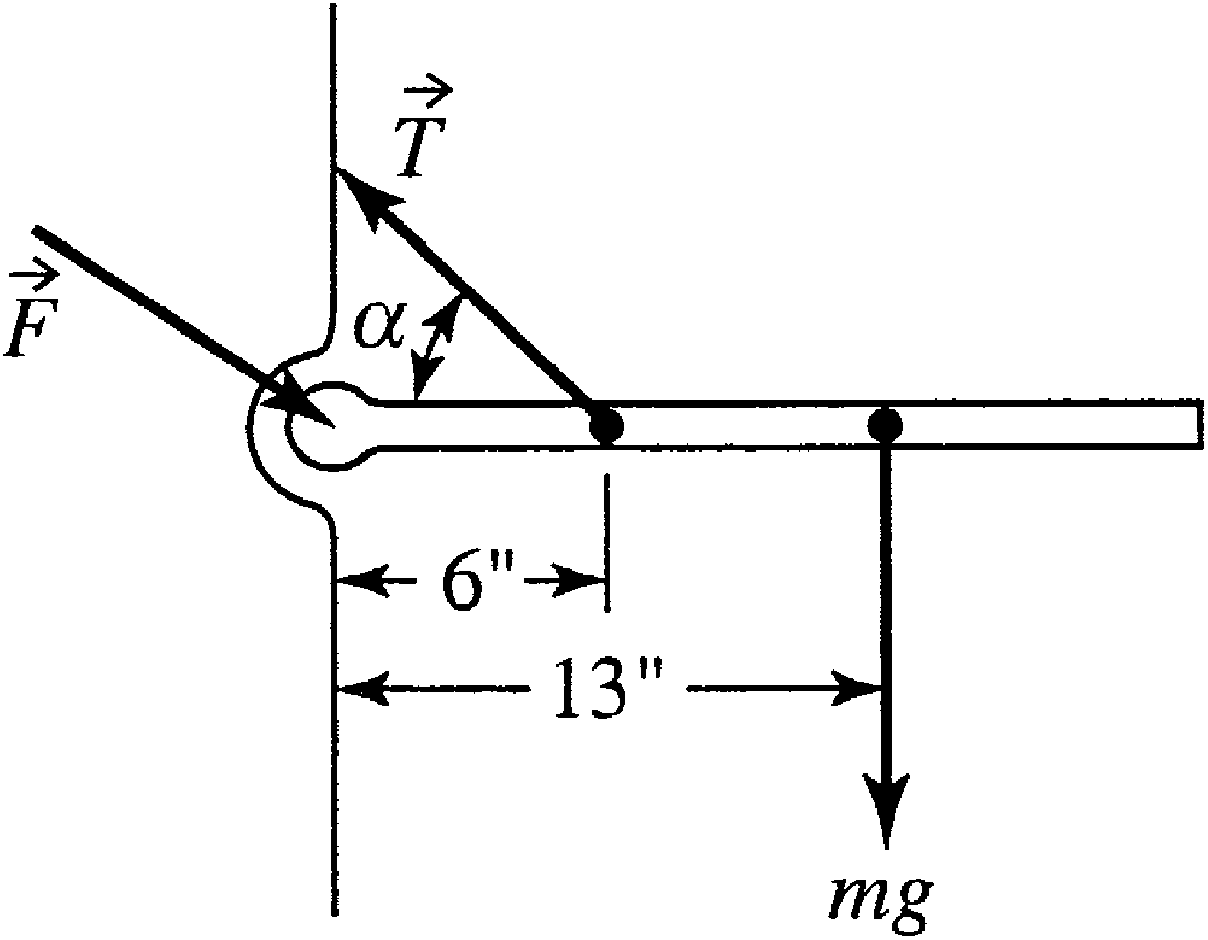
\includegraphics[width=0.5\textwidth]{254.png}
  \caption{Diagrama de fuerzas para el músculo deltoides y fuerzas de reacción durante el levantamiento con un brazo extendido. (Esta es una versión más simple de la Fig. 2.21). (De \cite{3}). Para el Problema 2.16.}
  \label{fig:254}
\end{SCfigure}

 Utilice las tres condiciones de equilibrio para determinar la tensión $T$ en el músculo deltoides necesaria para lograr este equilibrio, y las componentes vertical y horizontal de la fuerza ejercida por la escápula (omóplato) sobre el húmero. Asuma que el peso del húmero es $mg = 8\text{ lb}$ y que el músculo deltoides forma un ángulo $\alpha = 17^\circ$ con el húmero. (De \cite{3}).

\item[2.17] Resuelva el problema más general del hombro con un peso en la mano, representado en la Fig. 2.21, hallando $M$, $R$ y $\beta$. Ahora evalúe las componentes $x$ e $y$ de la fuerza muscular, la magnitud de la fuerza de reacción de la articulación y su ángulo para los siguientes parámetros: $a = 15\text{ cm}$, $b = 30\text{ cm}$, $c = 60\text{ cm}$, $\theta = 15^\circ$, $W = 40\text{ N}$ y $W_0 = 60\text{ N}$.

\item[2.18] (a) Un gimnasta de masa $m_b$ se suspende en las anillas con su cuerpo erguido y brazos rectos horizontales con los que sujeta las anillas. Cada anilla está suspendida por una cuerda con tensión $T$ que forma un ángulo agudo $\theta$ con sus brazos, y las anillas están separadas por una distancia $d$. Resuelva para $T$ y $\theta$. Asuma simetría.

(b) Si el gimnasta pesa $600\text{ N}$, $\theta = 75^\circ$ y $d = 1,8\text{ m}$, halle $T$. (De \cite{14}).

\item[2.19] Deduzca las ecuaciones (2.34)--(2.36) para el equilibrio de la pierna inferior con un peso en el tobillo.

\item[2.20] Determine el ángulo entre la pierna y la fuerza de reacción en la rodilla para las condiciones dadas en el texto para la Fig. 2.24.

\item[2.21] Analice cómo el tendón patelar y las fuerzas de reacción dependen del peso en el tobillo (para un peso de pierna fijo) y del ángulo de la pierna para la Fig. 2.24. Durante el ejercicio, ¿cuáles son las ventajas de variar este peso en comparación con este ángulo?

\item[2.22] Considere el equilibrio del pie durante la agachadilla (posición acuclillada) para una persona de $200\text{ lb}$, con la fuerza a través del tendón de Aquiles, la fuerza de reacción de la tibia y la fuerza normal del suelo en equilibrio, como en la Fig. 2.55 (ignorando el peso del pie por simplicidad). Tome el ángulo $\alpha = 38^\circ$.

\begin{SCfigure}[0.5][htbp]

  \centering
  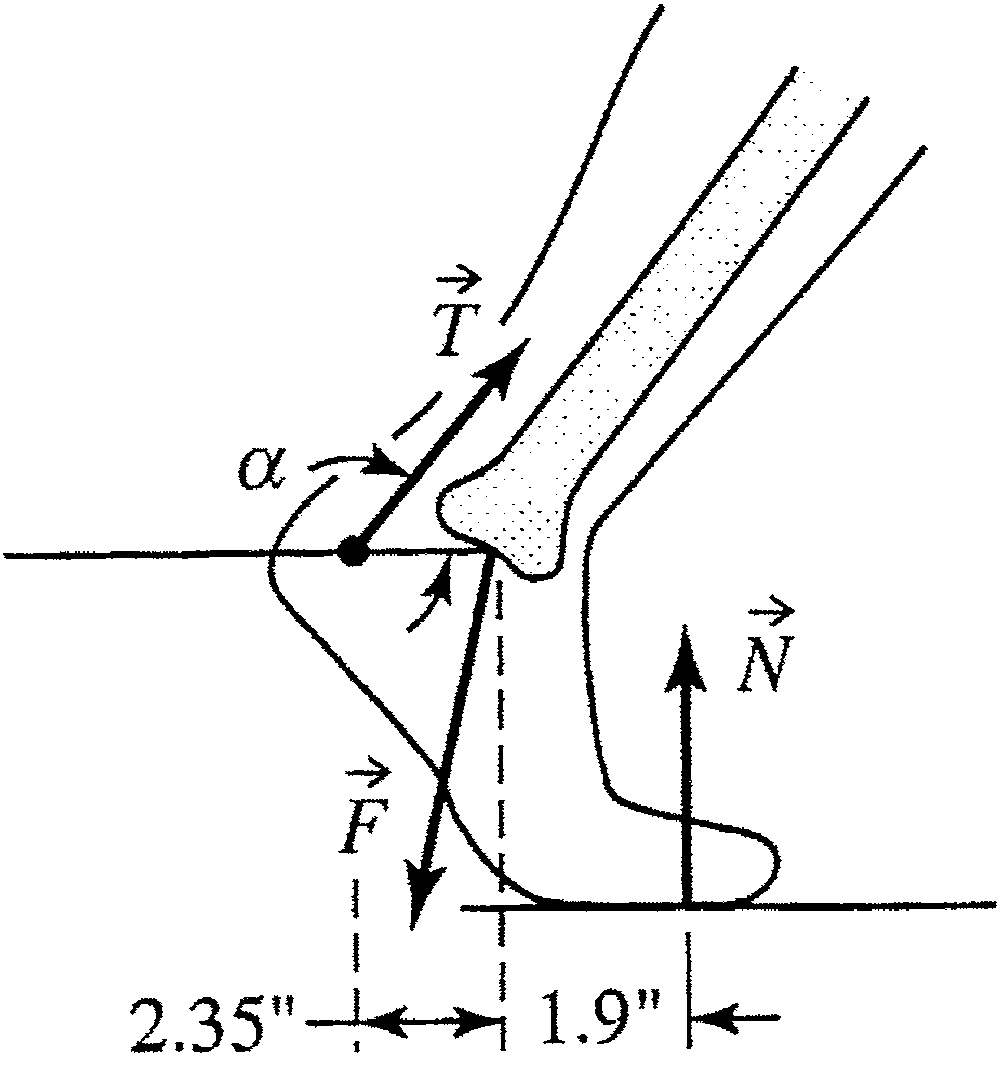
\includegraphics[width=0.55\textwidth]{255.png}
  \caption{Fuerzas sobre el pie durante la agachadilla (posición acuclillada). (De \cite{3}). Para el Problema 2.22.}
  \label{fig:255}
\end{SCfigure}



(a) ¿Por qué la fuerza normal del suelo es de $100\text{ lb}$?

(b) Halle la magnitud de la tensión del tendón de Aquiles $T$, y la magnitud y dirección de la fuerza de reacción $\vec{\mathbf{F}}$.

\item[2.23] El tema del Problema 2.22 es similar a la discusión de las fuerzas sobre el pie en el Cap. 3, donde asumiremos que todas las fuerzas son paralelas o antiparalelas entre sí y normales a una barra, como en una palanca. ¿Es esto totalmente válido? ¿Por qué sí o por qué no?

\item[2.24] Repita el Problema 2.22, incluyendo ahora la masa del pie. La distancia desde la parte inferior de la tibia (de donde emana la fuerza normal) es de $4\text{ in}$ y el centro de masa del pie está a la mitad de camino entre ella y el suelo. Utilice los datos para la masa del pie en el Cap. 1.

\item[2.25] En la posición de agachadilla, la pierna inferior se mantiene en equilibrio mediante la acción del ligamento patelar, que está unido a la parte superior de la tibia y pasa sobre la rótula. Como se representa en la Fig. 2.56, las fuerzas que actúan sobre la pierna inferior son $\vec{\mathbf{N}}$, $\vec{\mathbf{R}}$ y $\vec{\mathbf{T}}$. Si la pierna inferior está en equilibrio, determine la magnitud de la tensión $T$ en el ligamento patelar, y la dirección y magnitud de $\vec{\mathbf{R}}$. Asuma que la tensión actúa en un punto directamente debajo del punto de acción de $\vec{\mathbf{R}}$. Tome la fuerza normal igual a $100\text{ lb}$ (la mitad del peso corporal), el peso de la pierna $W_{\text{pierna}}$ como $20\text{ lb}$ y el ángulo $\alpha = 40^\circ$ (para la pierna a un ángulo de $45^\circ$). (De \cite{3}).

\begin{SCfigure}[0.5][htbp]

  \centering
  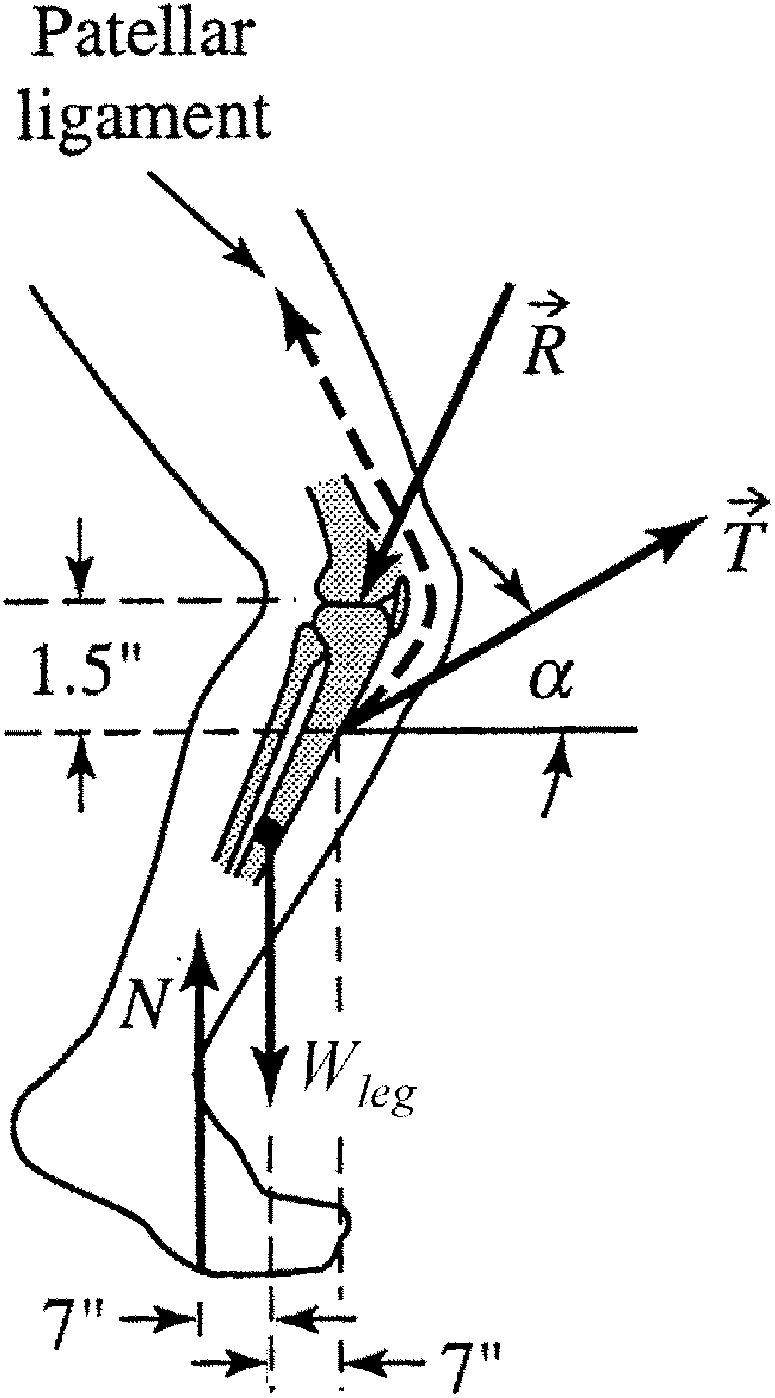
\includegraphics[width=0.5\textwidth]{256.png}
  \caption{Fuerzas sobre la pierna inferior durante la agachadilla (posición acuclillada). (De \cite{3}). Para el Problema 2.25.}
  \label{fig:256}
\end{SCfigure}



\item[2.26] Deduzca las ecuaciones (2.37) y (2.38) para el equilibrio de la rótula (patela).

\item[2.27] Deduzca las ecuaciones (2.39) y (2.40) para el equilibrio del pie.

\item[2.28] Las distancias laterales desde la articulación temporomandibular hasta la inserción de los músculos maseteros, los primeros premolares y los incisivos centrales son $0,4 L$, $L$ y $1,2 L$, respectivamente.

(a) ¿Qué tipo de palanca está involucrada al morder y masticar con los músculos maseteros?

(b) Para una mordida en equilibrio con una fuerza del músculo masetero de $1.625\text{ N}$, demuestre que la fuerza sobre el primer premolar es de $650\text{ N}$, asumiendo que no hay fuerza sobre los incisivos centrales \cite{5}. Dibuje un diagrama de fuerzas para esto.

(c) Bajo estas condiciones, demuestre que la fuerza opuesta necesaria sobre los incisivos centrales es de $540\text{ N}$, asumiendo ahora que no hay fuerza sobre el primer premolar. Dibuje un diagrama de fuerzas para esto.

\item[2.29] Cuando muerde una manzana solo con sus incisivos, ejerce una fuerza de $650\text{ N}$ sobre ella. Cuando muerde una manzana solo con sus premolares, ejerce una fuerza de $540\text{ N}$ sobre ella. Halle la fuerza por unidad de área (que se denomina esfuerzo o estrés) sobre la manzana para ambos casos si las áreas de contacto efectivas de los incisivos y premolares son de $5\text{ mm}^2$ y $1\text{ mm}^2$, respectivamente.

\subsection*{Estática de la espalda}

\item[2.30] Al analizar la inclinación del cuerpo, asumimos que el peso del tronco (por encima de las caderas, excluyendo los brazos y la cabeza) es $W_1 = 0,4 W_b$ y el peso de los brazos y la cabeza es $W_2 = 0,2 W_b$. ¿Es esto razonable? ¿Por qué?

\item[2.31] Considere a una mujer de $1,6\text{ m}$ de estatura y masa de $50\text{ kg}$.

(a) Calcule la fuerza de reacción sobre sus vértebras inferiores y la fuerza en su músculo erector de la columna cuando está erguida o inclinada a $60^\circ$ (y consecuentemente a $30^\circ$ respecto a la horizontal).

(b) Vuelva a calcular estas fuerzas cuando esté embarazada. Asuma que durante el embarazo la masa de su torso aumenta en $15\text{ kg}$, pero el centro de masa del torso es el mismo.

(c) ¿Las fuerzas en la parte (b) son equivalentes a las de la misma mujer no embarazada que levanta un peso de qué masa?

\item[2.32] Describa los diseños del respaldo de una silla que podrían provocar dolor en las vértebras lumbares y aquellos que proporcionarían un buen soporte lumbar.

\item[2.33] Demostramos que cuando la fuerza sobre el disco lumbosacro (intervertebral) aumenta de $0$ a $2.400\text{ N}$, la altura del disco $H$ disminuye en un $20\%$ y el radio del disco $r$ aumenta en aproximadamente un $10\%$. Cuando se reconoce que la carga sobre el disco para una persona vertical es en realidad de $530\text{ N}$ (y no $0$), ¿cómo cambian realmente las dimensiones del disco cuando la persona se inclina a un ángulo de $30^\circ$ (y por ende a una carga de $2.400\text{ N}$)?

\item[2.34] ¿Por qué es más difícil levantar objetos voluminosos? Una persona levanta un paquete de masa $20\text{ kg}$ frente a ella de modo que la parte posterior del paquete toca su abdomen. La distancia horizontal desde el disco lumbosacro de la persona hasta la parte frontal de su abdomen es de $20\text{ cm}$. Calcule los momentos de flexión (en $\text{N}\cdot\text{m}$) alrededor del centro de masa de su disco causados por las cargas levantadas, asumiendo que el paquete tiene alternativamente $20$ o $40\text{ cm}$ de profundidad \cite{25}. Dibuje diagramas de fuerzas para estos dos casos. Las otras dimensiones de los paquetes son las mismas y ambos tienen densidad uniforme. ¿Cómo muestra esto que el tamaño del objeto levantado afecta la carga sobre la columna lumbar?

\item[2.35] ¿Por qué es mejor estar erguido cuando se sostiene un objeto? Una persona sostiene un objeto de $20\text{ kg}$ mientras está erguida o inclinada hacia adelante. La masa de la persona por encima de su disco lumbosacro (su torso) es de $45\text{ kg}$. Cuando está erguido, el centro de masa del torso está (horizontalmente) a $2\text{ cm}$ frente a su disco y el del objeto está a $30\text{ cm}$ frente a su disco. Cuando está inclinado, el centro de masa del torso está a $25\text{ cm}$ frente a su disco y el del objeto está a $40\text{ cm}$ frente a su disco. Dibuje diagramas de fuerzas para estos dos casos. Calcule los momentos de flexión (en $\text{N}\cdot\text{m}$) alrededor del centro de masa de su disco causados por sostener esta carga ya sea estando erguido o inclinado \cite{25}. ¿Cómo muestra esto que inclinarse al levantar un objeto afecta la carga sobre la columna lumbar?

\item[2.36] ¿Por qué es mejor levantar un objeto con las piernas dobladas y el objeto muy cerca de usted? Una persona levanta un objeto de $20\text{ kg}$ ya sea inclinándose con las piernas rectas, con las rodillas dobladas y el objeto cerca de su cuerpo, o con las rodillas dobladas y el objeto lejos de su cuerpo. La masa de la persona por encima de su disco lumbosacro (su torso) es de $45\text{ kg}$. Cuando se inclina con las piernas rectas, el centro de masa de su torso está (horizontalmente) a $25\text{ cm}$ frente a su disco y el del objeto está a $40\text{ cm}$ frente a su disco. Cuando se inclina con las rodillas dobladas y el objeto cerca de su cuerpo, el centro de masa de su torso está (horizontalmente) a $18\text{ cm}$ frente a su disco y el del objeto está a $35\text{ cm}$ frente a su disco. Cuando se inclina con las rodillas dobladas y el objeto lejos de su cuerpo, el centro de masa de su torso está (horizontalmente) a $25\text{ cm}$ frente a su disco y el del objeto está a $50\text{ cm}$ frente a su disco. Dibuje diagramas de fuerzas para estos tres casos. Calcule los momentos de flexión (en $\text{N}\cdot\text{m}$) alrededor del centro de masa de su disco para estos tres métodos de levantamiento \cite{25}. ¿Qué posición es la peor? ¿Cómo muestra esto que la posición al levantar un objeto afecta la carga sobre la columna lumbar?

\item[2.37] Una posición durante el paleo de nieve o tierra se muestra en la Fig. 2.57. Asuma que esta es una posición de equilibrio.

\begin{SCfigure}[0.5][htbp]

  \centering
  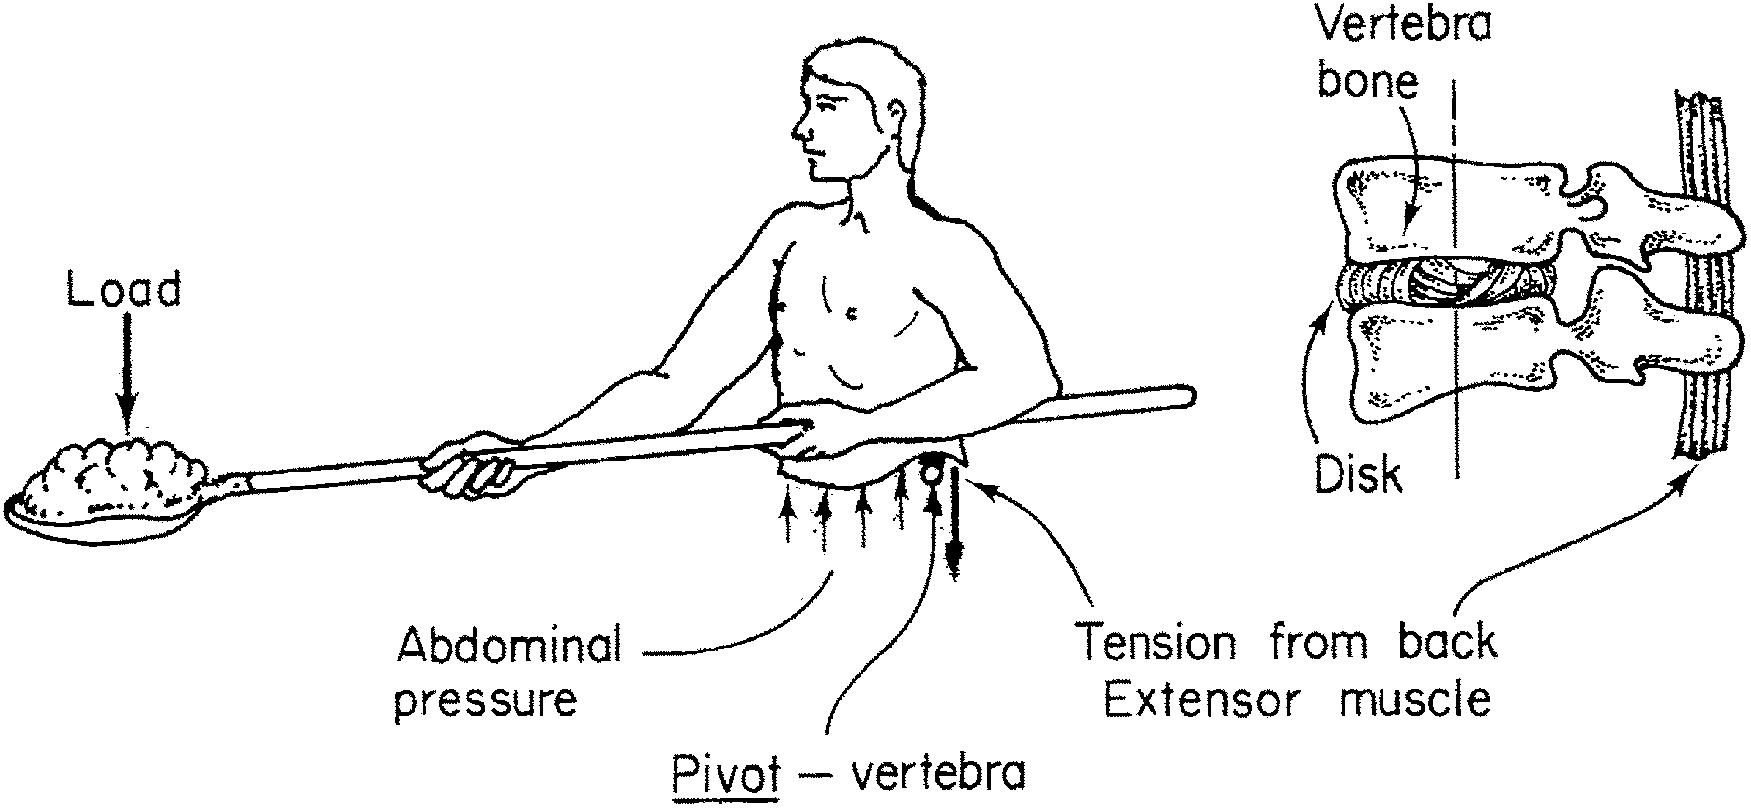
\includegraphics[width=0.55\textwidth]{257.png}
  \caption{Acción de palear (quitar nieve o tierra con pala). (De \cite{11}). Para el Problema 2.37.}
  \label{fig:257}
\end{SCfigure}



(a) Si la pala y su contenido tienen una masa de $10\text{ kg}$, con un centro de masa a $1\text{ m}$ de la vértebra lumbar, halle el momento respecto a esa vértebra.

(b) Si los músculos de la espalda están a $5\text{ cm}$ detrás del centro del disco, halle la magnitud y dirección de la fuerza muscular necesaria para el equilibrio.

(c) Halle la fuerza sobre el disco intervertebral.

(d) Si los músculos abdominales de la persona son fuertes y pueden proporcionar cierta fuerza hacia arriba, ¿ayudaría eso a aliviar el esfuerzo sobre los músculos de la espalda y el disco? ¿Por qué?

\subsection*{Modelado multisegmento}

\item[2.38] (a) Dibuje un modelo de segmentos articulados (en el plano) de la pierna que muestre las fuerzas sobre el muslo, la pantorrilla y el tobillo, utilizando las fuerzas resultantes de la Fig. 2.58. Muestre las fuerzas de gravedad del centro de masa en cada segmento, junto con las fuerzas normales (en cada articulación del cuerpo y con el suelo).

\begin{SCfigure}[0.5][htbp]

  \centering
  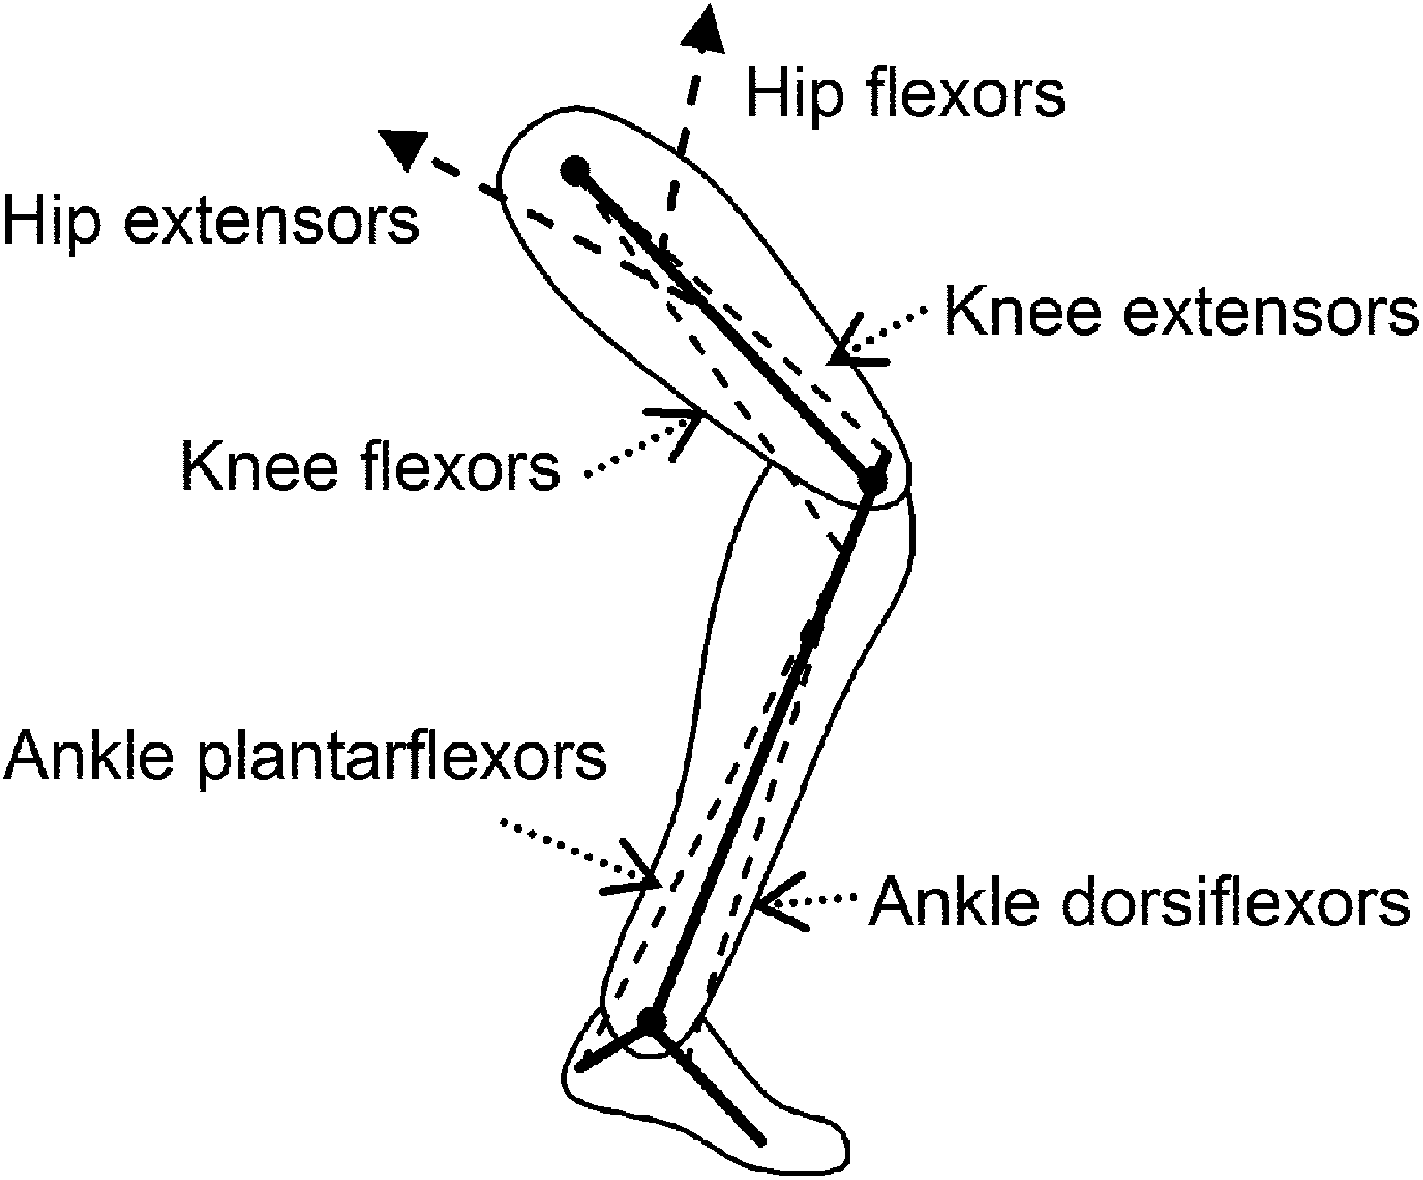
\includegraphics[width=0.55\textwidth]{258.png}
  \caption{Fuerzas resultantes idealizadas para seis grupos musculares en la pierna. (Basado en \cite{19}). Para el Problema 2.38.}
  \label{fig:258}
\end{SCfigure}



(b) Etiquete todas las distancias y ángulos necesarios para analizar las fuerzas y torques en el plano. Para cada segmento, etiquete las distancias comenzando desde el extremo proximal. Etiquete cada ángulo entre músculo y hueso; use los ángulos como se muestran, con el ángulo agudo cuando sea posible.

(c) Escriba el equilibrio de fuerzas y la ecuación de torque para cada uno de los segmentos.

(d) Para cada una de estas condiciones de equilibrio, sume las ecuaciones (como las ecuaciones de torque) para el muslo, la pantorrilla y el pie. Demuestre que las tres ecuaciones de equilibrio resultantes son las ecuaciones correctas para toda la pierna.

\subsection*{El sentido del tacto}

\item[2.39] (a) Una persona de $50\text{ kg}$ se para sobre las puntas de sus dedos. Asumiendo que cada dedo hace un área de contacto de $1\text{ cm}^2$ con el suelo, halle la presión en cada punta de los dedos.

(b) ¿Qué sensores táctiles están percibiendo esta presión?
\end{enumerate}

\section*{Referencias}

\begin{thebibliography}{99}
\bibitem{1} M.A. Adams, K. Burton, P. Dolan, N. Bogduk, \textit{The Biomechanics of Back Pain}, 2.ª ed. (Churchill-Livingstone, Edimburgo, 2006)
\bibitem{2} G.B.J. Andersson, R. Örtengren, A. Nachemson, G. Elfström, Lumbar disc pressure and myoelectric back activity during sitting. 1. studies on an experimental chair. \textit{Scand. J. Rehabil. Med.} \textbf{3}, 104--114 (1974)
\bibitem{3} G.B. Benedek, F.M.H. Villars, \textit{Physics with Illustrative Examples from Medicine and Biology}, vol. 3, 2.ª ed. (AIP/Springer, Berlín, 2000)
\bibitem{4} B.H. Brown, R.H. Smallwood, D.C. Barber, P.V. Lawford, D.R. Hose, \textit{Medical Physics and Biomedical Engineering} (Institute of Physics, Filadelfia, 1999)
\bibitem{5} J.R. Cameron, J.G. Skofronick, R. Grant, \textit{Physics of the Body}, 2.ª ed. (Medical Physics, Madison, 1999)
\bibitem{6} A. Cappozzo, Compressive loads in the lumbar vertebral column during normal level walking. \textit{J. Orthop. Res.} \textbf{1}, 292 (1984)
\bibitem{7} D.B. Chaffin, G.B.J. Andersson, B.J. Martin, \textit{Occupational Biomechanics}, 3.ª ed. (Wiley-Interscience, Nueva York, 1999)
\bibitem{8} K.M. Dunn, P.R. Croft: Epidemiology and natural history of low back pain. \textit{Europa Medicophysica} (ahora \textit{Eur. J. Phys. Rehab. Med.}). \textbf{40}, 9--13 (2004)
\bibitem{9} R.M. Enoka, \textit{Neuromechanics of Human Movement}, 4.ª ed. (Human Kinetics, Champaign, 2008)
\bibitem{10} Y.C. Fung, \textit{Biomechanics: Motion, Flow, Stress, and Growth} (Springer, Berlín, 1990)
\bibitem{11} Y.C. Fung, \textit{Biomechanics: Mechanical Properties of Living Tissues}, 2.ª ed. (Springer, Berlín, 1993)
\bibitem{12} S. Garfield, \textit{Teeth, Teeth, Teeth: A Thorough Treatise} (Simon \& Schuster, Nueva York, 1969)
\bibitem{13} E.B. Goldstein, \textit{Sensation and Perception}, 4.ª ed. (Brooks/Cole, Pacific Grove, 1996)
\bibitem{14} J.G. Hay, \textit{The Biomechanics of Sports Techniques}, 4.ª ed. (Prentice-Hall, Englewood Cliffs, 1993)
\bibitem{15} B. Le Veau, \textit{Williams and Lissner: Biomechanics of Human Motion}, 2.ª ed. (Saunders, Filadelfia, 1977)
\bibitem{16} D.E. Lieberman, \textit{The Evolution of the Human Head} (Harvard University Press, Cambridge, 2011)
\bibitem{17} D.E. Lieberman, \textit{The Story of the Human Body: Evolution, Health, and Disease} (Pantheon, Nueva York, 2013)
\bibitem{18} R.B. Martin, D.B. Burr, N.A. Sharkey, \textit{Skeletal Tissue Mechanics} (Springer, Berlín, 1998)
\bibitem{19} D.I. Miller, R.C. Nelson, \textit{Biomechanics of Sport: A Research Approach} (Lea \& Febiger, Filadelfia, 1973)
\bibitem{20} K.L. Moore, A.M.R. Agur, \textit{Essential Clinical Anatomy}, 2.ª ed. (Lippincott Williams \& Wilkins, Filadelfia, 2002)
\bibitem{21} K.L. Moore, A.M.R. Agur, \textit{Essential Clinical Anatomy}, 3.ª ed. (Lippincott Williams \& Wilkins, Filadelfia, 2007)
\bibitem{22} A. Nachemson, Towards a better understanding of back pain: a review of the mechanics of the lumbar disk. \textit{Rheumatol. Rehabil.} \textbf{14}, 129 (1975)
\bibitem{23} R. Nanda (ed.), \textit{Biomechanics in Clinical Orthodontics} (Saunders, Filadelfia, 1997)
\bibitem{24} M. Nordin, V.H. Frankel (eds.), \textit{Basic Biomechanics of the Musculoskeletal System}, 3.ª ed. (Lippincott Williams \& Wilkins, Filadelfia, 2001)
\bibitem{25} M. Nordin, S.S. Weiner, M. Lindh, Biomechanics of the lumbar spine. En \textit{Basic Biomechanics of the Musculoskeletal System}, 3.ª ed., editado por M. Nordin, V.H. Frankel (Lippincott Williams \& Wilkins, Filadelfia, 2001), pp. 256--284. Cap. 10
\bibitem{26} M. Nordin, V.H. Frankel (eds.), Biomechanics of the knee. En \textit{Basic Biomechanics of the Musculoskeletal System}, 3.ª ed. (Lippincott Williams \& Wilkins, Filadelfia, 2001), pp. 176--201. Cap. 7
\bibitem{27} M. Nordin, V.H. Frankel (eds.), Biomechanics of the hip. En \textit{Basic Biomechanics of the Musculoskeletal System}, 3.ª ed. (Lippincott Williams \& Wilkins, Filadelfia, 2001), pp. 202--221. Cap. 8
\bibitem{28} N. Ozkaya, M. Nordin, \textit{Fundamentals of Biomechanics: Equilibrium, Motion, and Deformation}, 2.ª ed. (Springer, Berlín, 1999)
\bibitem{29} W.R. Proffit, H.W. Fields Jr., \textit{Contemporary Orthodontics}, 3.ª ed. (Mosby, St. Louis, 2000)
\bibitem{30} T.H. Schiebler, \textit{Anatomie}, 9.ª ed. (Springer, Berlín, 2005)
\bibitem{31} R.F. Schmidt, F. Lang, G. Thews, \textit{Physiologie des Menschen}, 29.ª ed. (Springer, Berlín, 2005)
\bibitem{32} F.G. Shaw, D.C. Scott, \textit{Practical Exercises in Dental Mechanics}, 3.ª ed. (Henry Kimpton, Londres, 1968)
\bibitem{33} C.J. Snijders, Engineering approaches to standing, sitting, and lying. En \textit{Basic Biomechanics of the Musculoskeletal System}, 3.ª ed., editado por M. Nordin, V.H. Frankel (Lippincott Williams \& Wilkins, Filadelfia, 2001), pp. 420--436. Cap. 17
\bibitem{34} G.S. Throckmorton, J.S. Dean, The relationship between jaw-muscle mechanical advantage and activity levels during isometric bites in humans. \textit{Arch. Oral Biol.} \textbf{39}, 429--437 (1994)
\bibitem{35} B.N. Tillmann, \textit{Atlas der Anatomie des Menschen} (Springer, Berlín, 2005)
\bibitem{36} G. Waddell, \textit{The Back Pain Revolution}, 2.ª ed. (Churchill-Livingstone, Edimburgo, 2004)
\bibitem{37} H.J. Wilke, P. Neef, M. Caimi et al., New in vivo measurements of pressures in the intervertebral disc in daily life. \textit{Spine} \textbf{24}, 755 (1999)
\bibitem{38} M. Williams, H.B. Lissner, \textit{Biomechanics of Human Motion} (Saunders, Filadelfia, 1962)
\bibitem{39} D.A. Winter, \textit{Biomechanics and Motor Control of Human Movement}, 3.ª ed. (Wiley, Nueva York, 2005)
\bibitem{40} H. Yamada, \textit{Strength of Biological Materials} (Williams \& Wilkins, Baltimore, 1970)
\end{thebibliography}

\end{document}

